%\documentclass[11pt]{amsart}
\documentclass[11pt]{article}
\usepackage[letterpaper,left=2.5cm,right=2cm,textheight=23.5cm]{geometry}                % See geometry.pdf to learn the layout options. There are lots.
%\geometry{letterpaper}                   % ... or a4paper or a5paper or ... 
%\geometry{landscape}                % Activate for for rotated page geometry
%\usepackage[parfill]{parskip}    % Activate to begin paragraphs with an empty line rather than an indent
\usepackage{graphicx}
\usepackage{amssymb}
\usepackage{epstopdf}
%\usepackage[margin=0.9in]{geometry}
%\setlength{textwidth}{7.0in}
\newcommand{\arcsec}{$^{\prime\prime}$}
%\usepackage[left=2cm, right=5cm, top=2cm]{geometry}
\DeclareGraphicsRule{.tif}{png}{.png}{`convert #1 `dirname #1`/`basename #1 .tif`.png}
\linespread{1.5}
\title{\bf Planning for Drift-Scan Spectra of LMC SNRs \\
(and H~II regions) from SOAR/Goodman \\
Dec 2018 - Jan 2019}
%\author{The Author}
\date{}                                           % Activate to display a given date or no date

\begin{document}
\maketitle
%\section{}
%\subsection{}
\vspace{1in}
\flushleft{In all images, each panel is 10 arcmin square, unless otherwise noted.

The panels are:
}

\flushleft{Ha subtracted \qquad  [S II] subtracted}
\vspace{2 mm}
\flushleft{Ha \qquad \qquad \qquad \   \  [S II]/Ha (0.25 = neutral grey)}\
\vspace{1cm}

\quad\quad\quad or in some cases (should be obvious)

\vspace{0.5cm}
\flushleft{Ha \qquad \qquad  \qquad \  \  \  \  [S II] subtracted}
\vspace{2 mm}
\flushleft{Red continuum \qquad [S II]/Ha (0.25 = neutral grey)}\

\vspace{0.5cm}

\flushleft{Notes:}

\textbullet \quad SNRs labeled ``Bxxxx-yy.y" all appear in Mathewson (1983, 84, or 85) and all have regions marked in BLUE .

\textbullet \quad Other previously cataloged SNRs have regions marked in RED.

\textbullet \quad New SNR candidates have regions marked in MAGENTA.

% \end{document}
\newpage
{\bf J0448-6700}

Slit Center:   4:48:03.839        -66:59:37.424      N-S

Scan:  East

Scan rate:  

Date/Frames:

Exposure Times:  

\begin{figure}
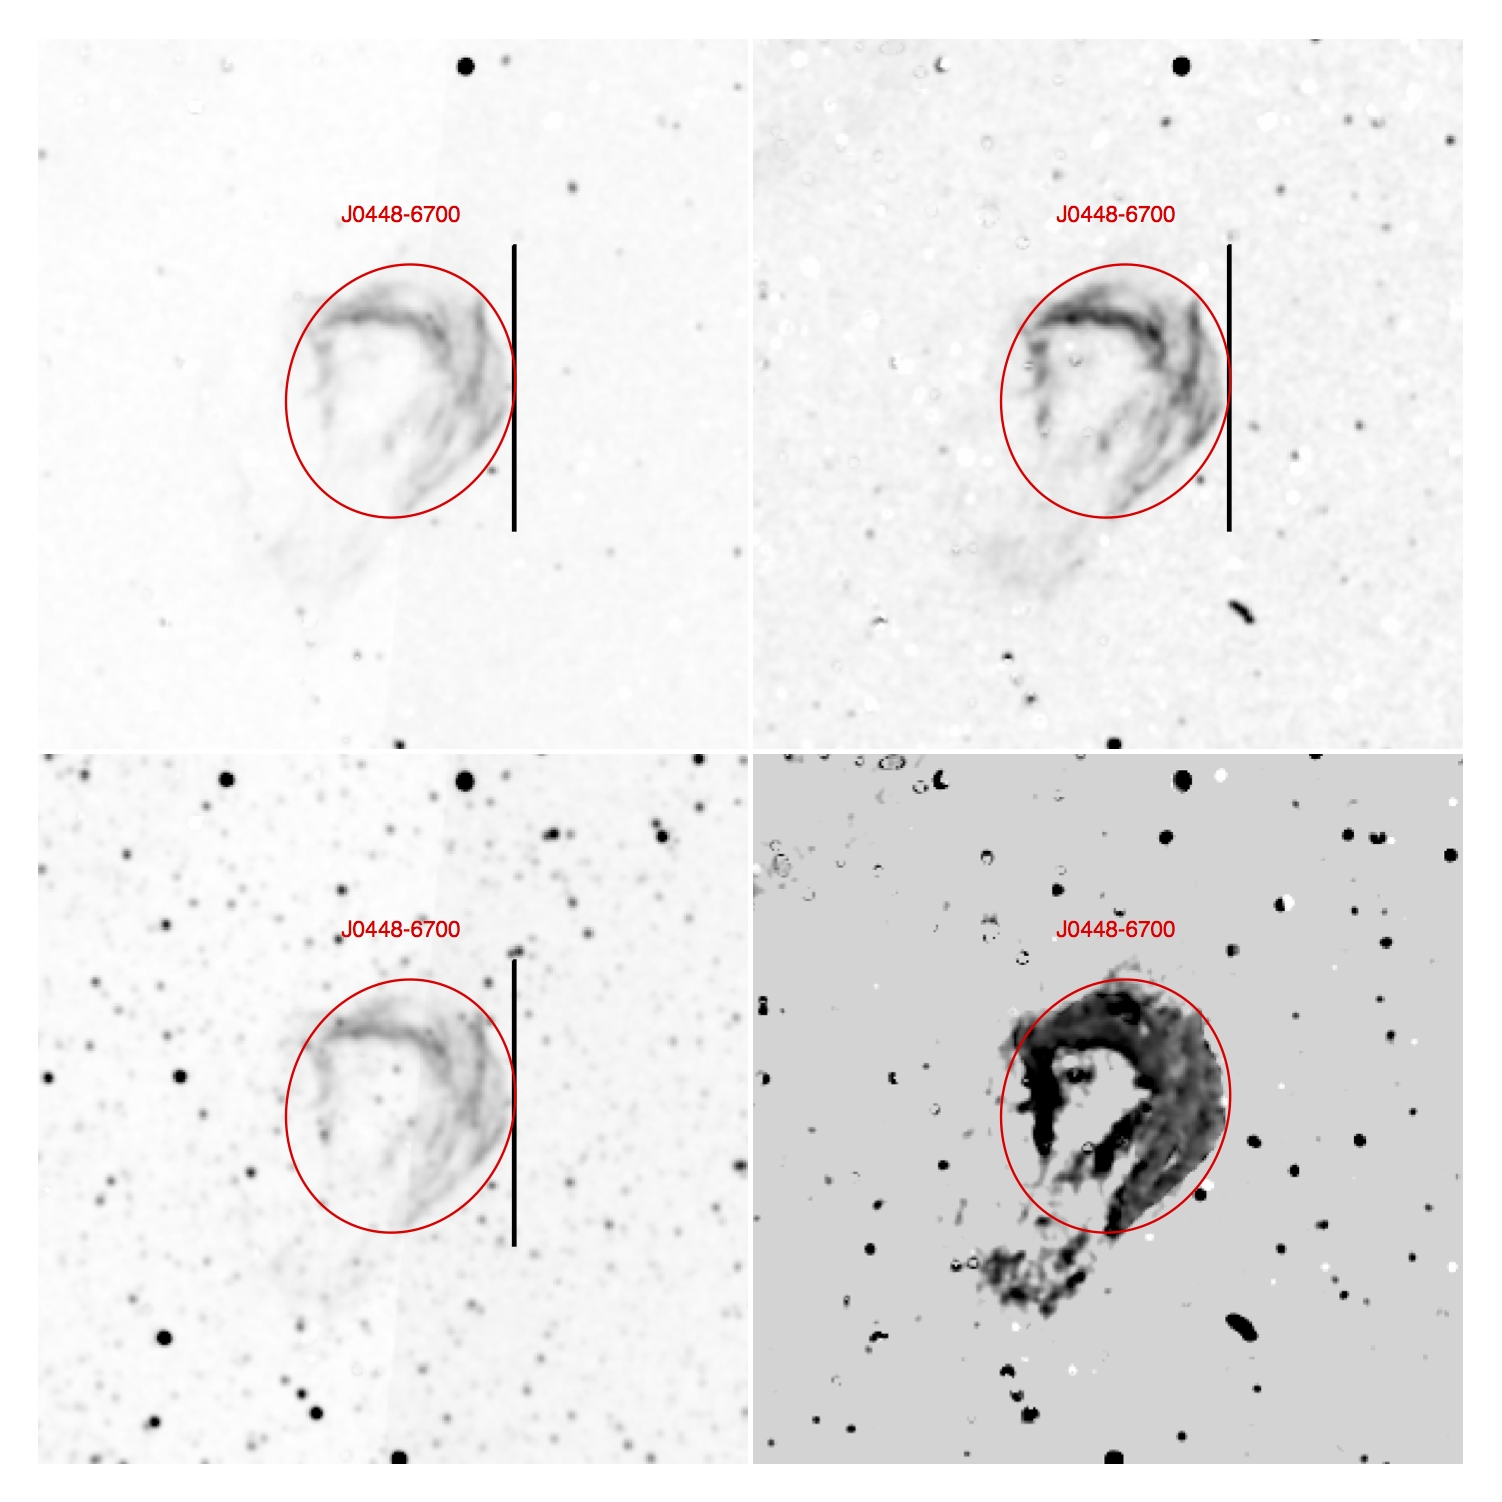
\includegraphics[width=11.cm]{snapshots/J0448-6700.png}
\end{figure}

\newpage
{\bf J0449-6920}

Slit Center:   4:49:12.574     -69:20:18.499     N-S

Scan:  East

Scan rate:  

Date/Frames:

Exposure Times:  

\begin{figure}
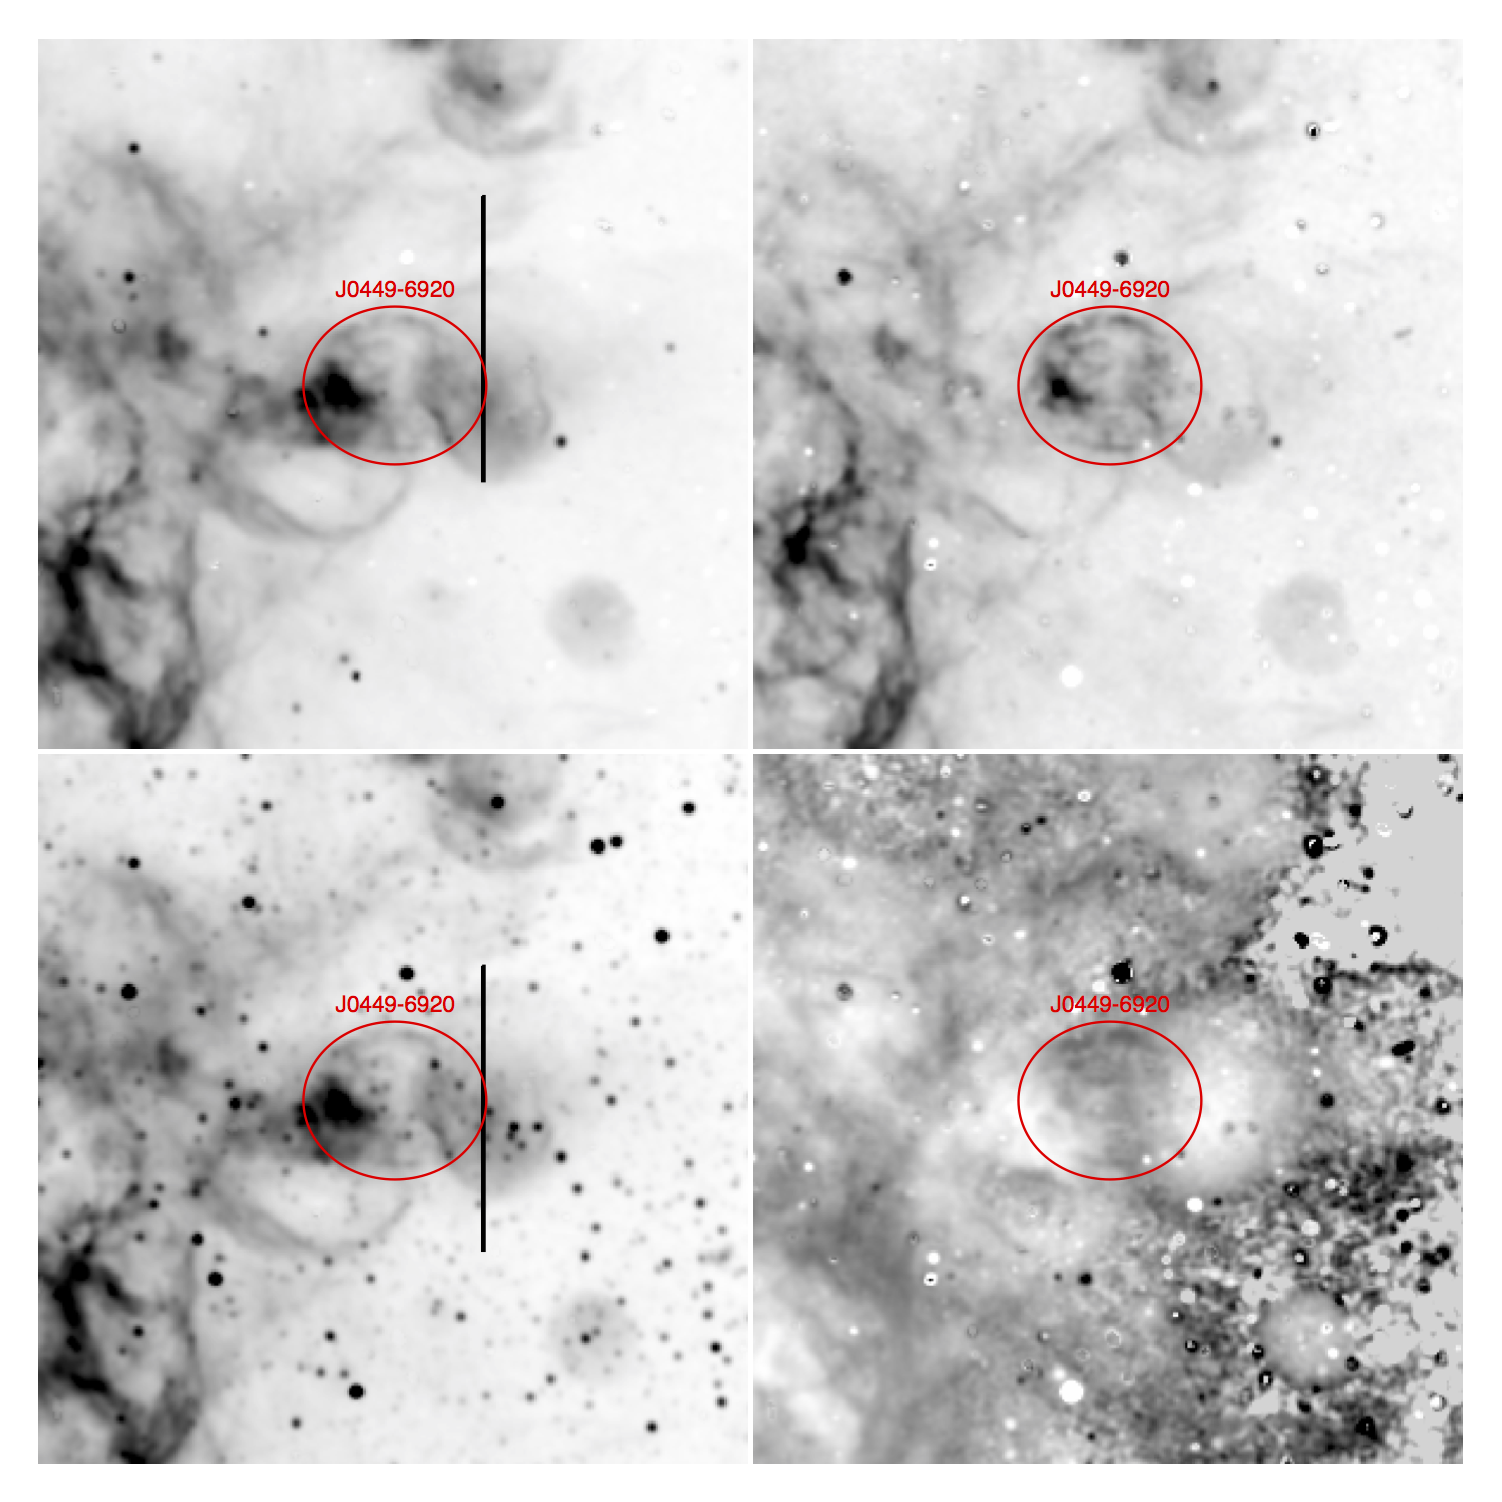
\includegraphics[width=11.cm]{snapshots/J0449-6920.png}
\end{figure}

\newpage
{\bf J0453-6655}

SNR Center:   4:53:14.3   -66:55:12.2     

N-S slit, center on bright star near west rim; then offset N 38$^{\prime\prime}$, E 5\arcsec.

Scan:  East  200$^{\prime\prime}$

Scan rate:  400$^{\prime\prime}$/hr for 30 min exposure

Date/Frames:  Night 3, frames 244-245 (only 2 at end of last night)

Exposure Times:  2 x 30 min

\begin{figure}
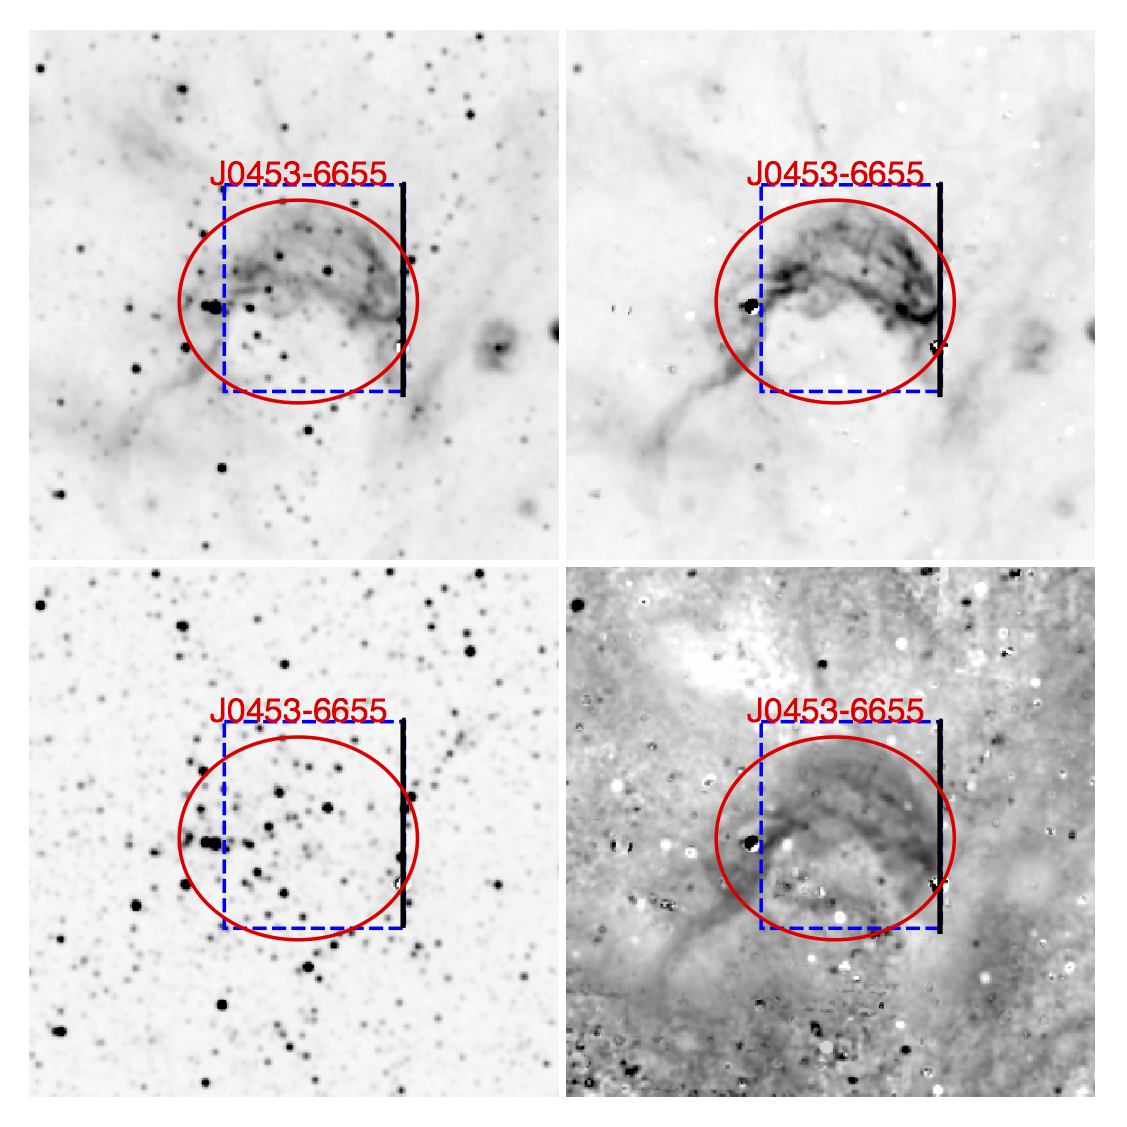
\includegraphics[width=12.5cm]{snapshots/J0453-6655a.png}
\end{figure}

%\end{document}


\newpage
{\bf J0453-6829 = B0453-685}

Slit Center:   4:53:14.089    -68:29:43.361     N-S

Scan:  East

Scan rate:  

Date/Frames:

Exposure Times:  

\begin{figure}
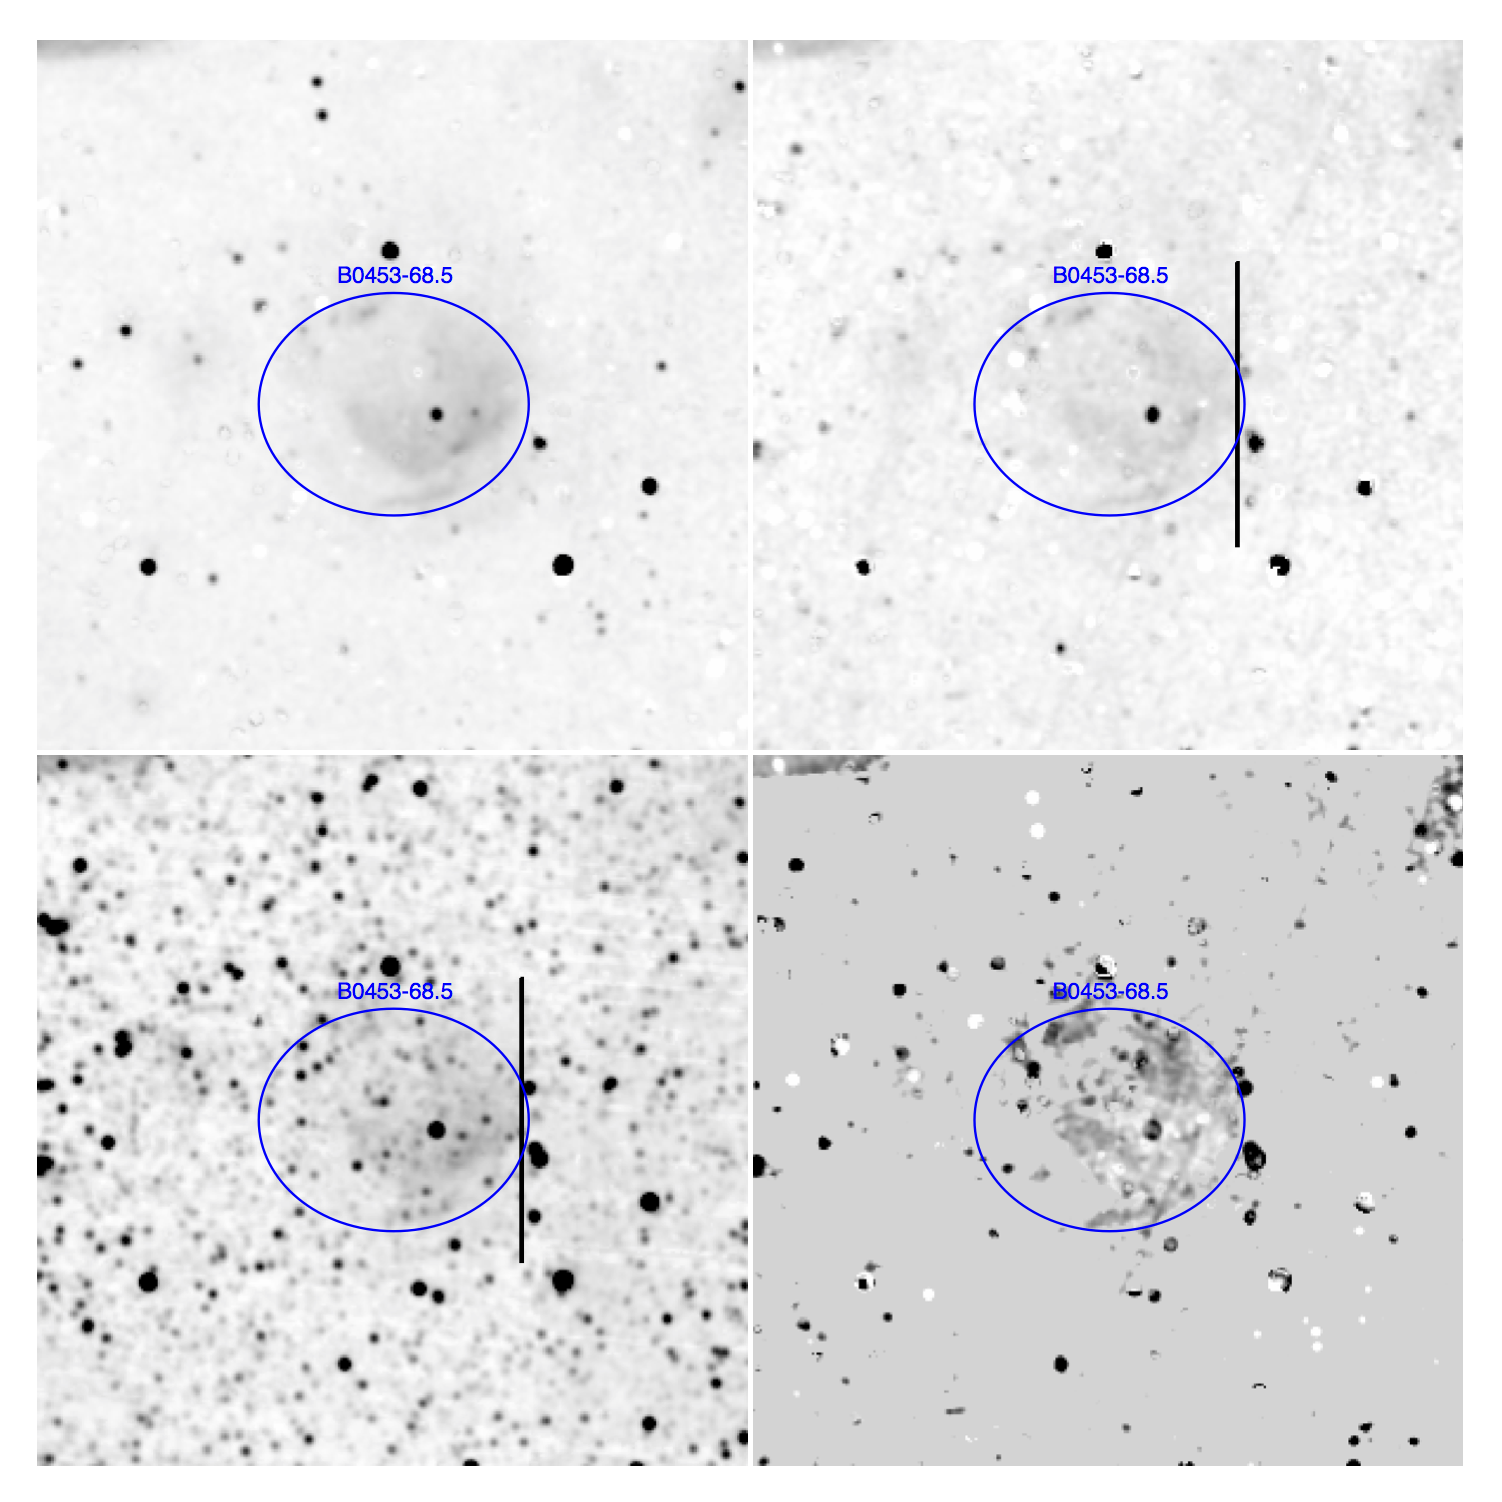
\includegraphics[width=11.cm]{snapshots/B0453-685.png}
\end{figure}

\newpage
{\bf JJ0454-7003 (new)}

Slit Center:   4:54:07.473      -70:04:07.707     N-S

Scan:  East

Scan rate:  

Date/Frames:

Exposure Times:  

\begin{figure}
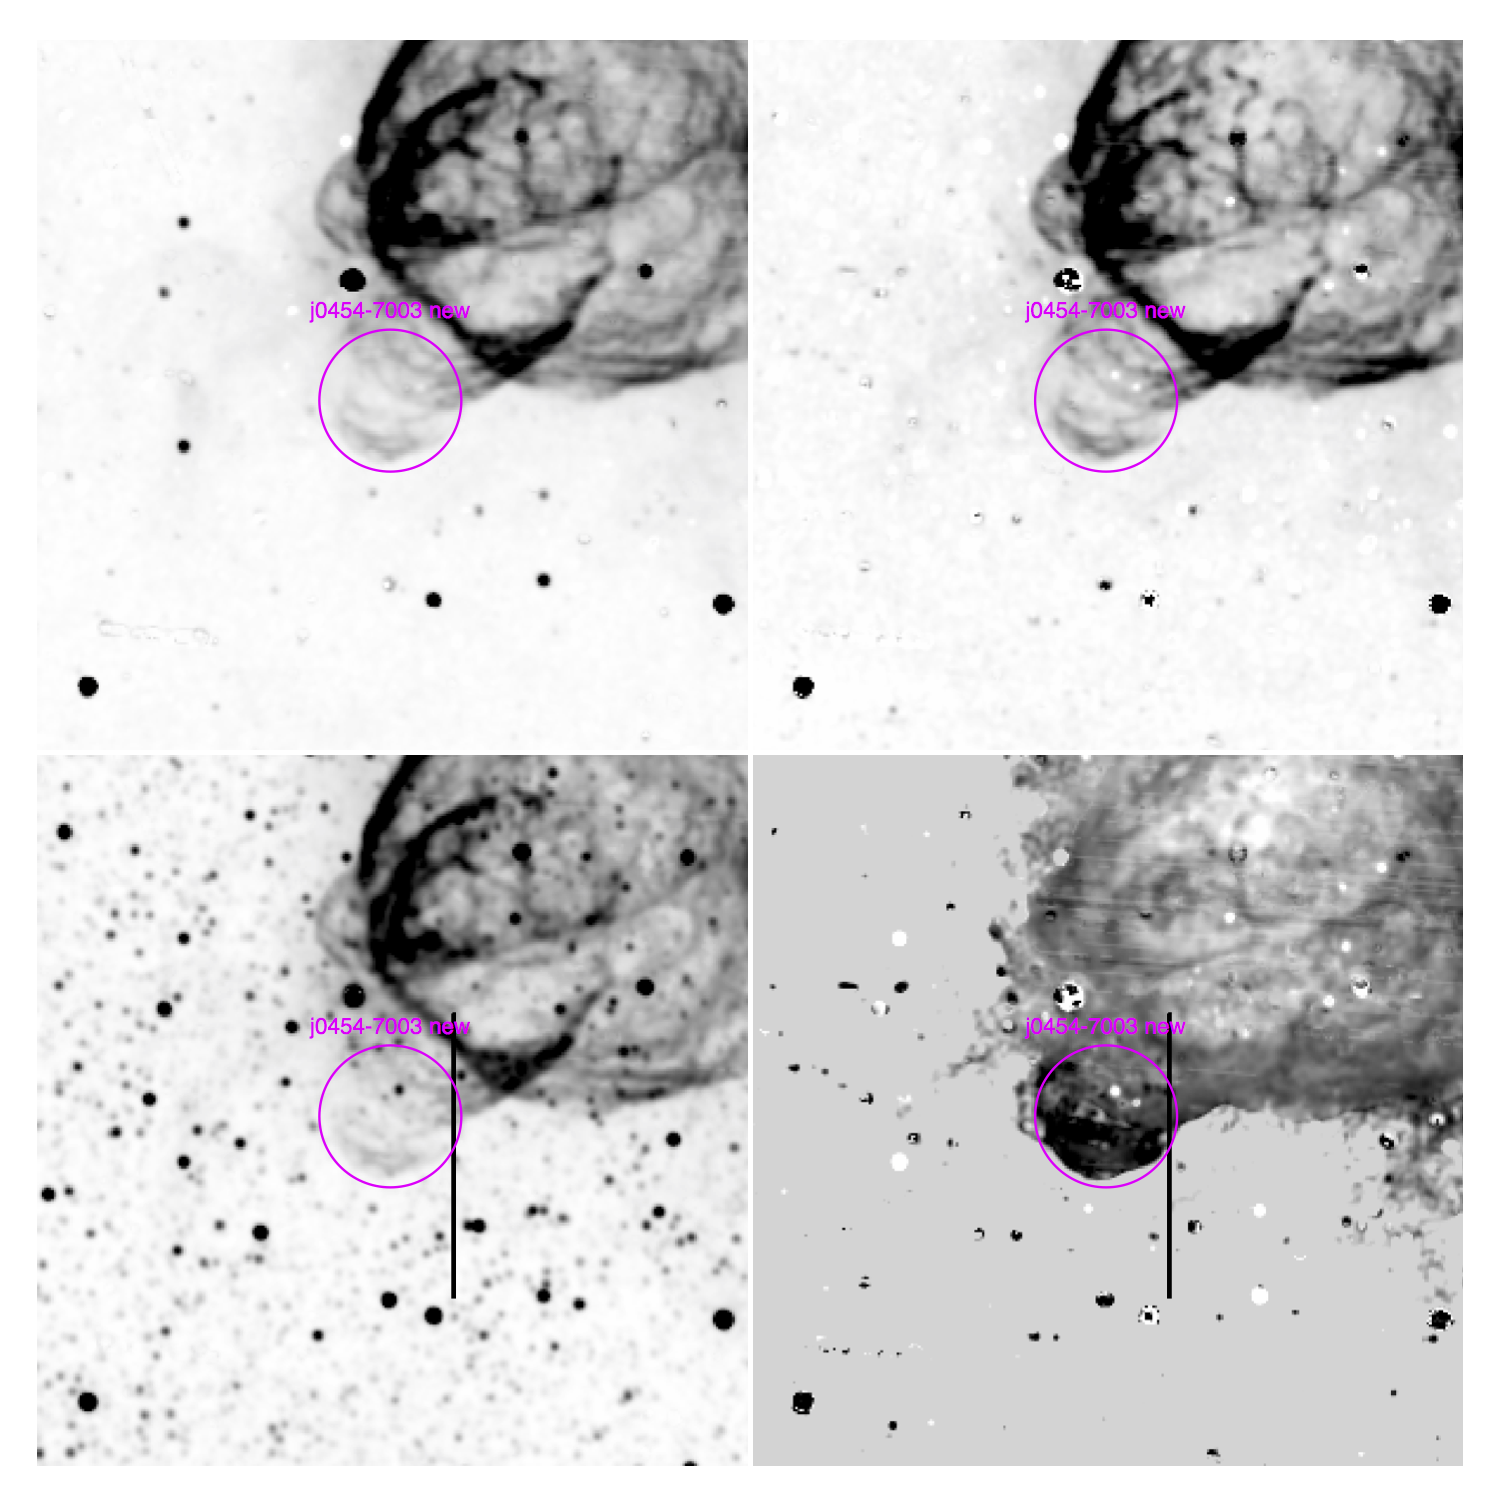
\includegraphics[width=11.cm]{snapshots/J0454-7003.png}
\end{figure}

\newpage
{\bf J0454-6712 = N9}

Slit Center:   4:54:17.308    -67:12:55.968     N-S

Scan:  East

Scan rate:  

Date/Frames:

Exposure Times:  

\begin{figure}
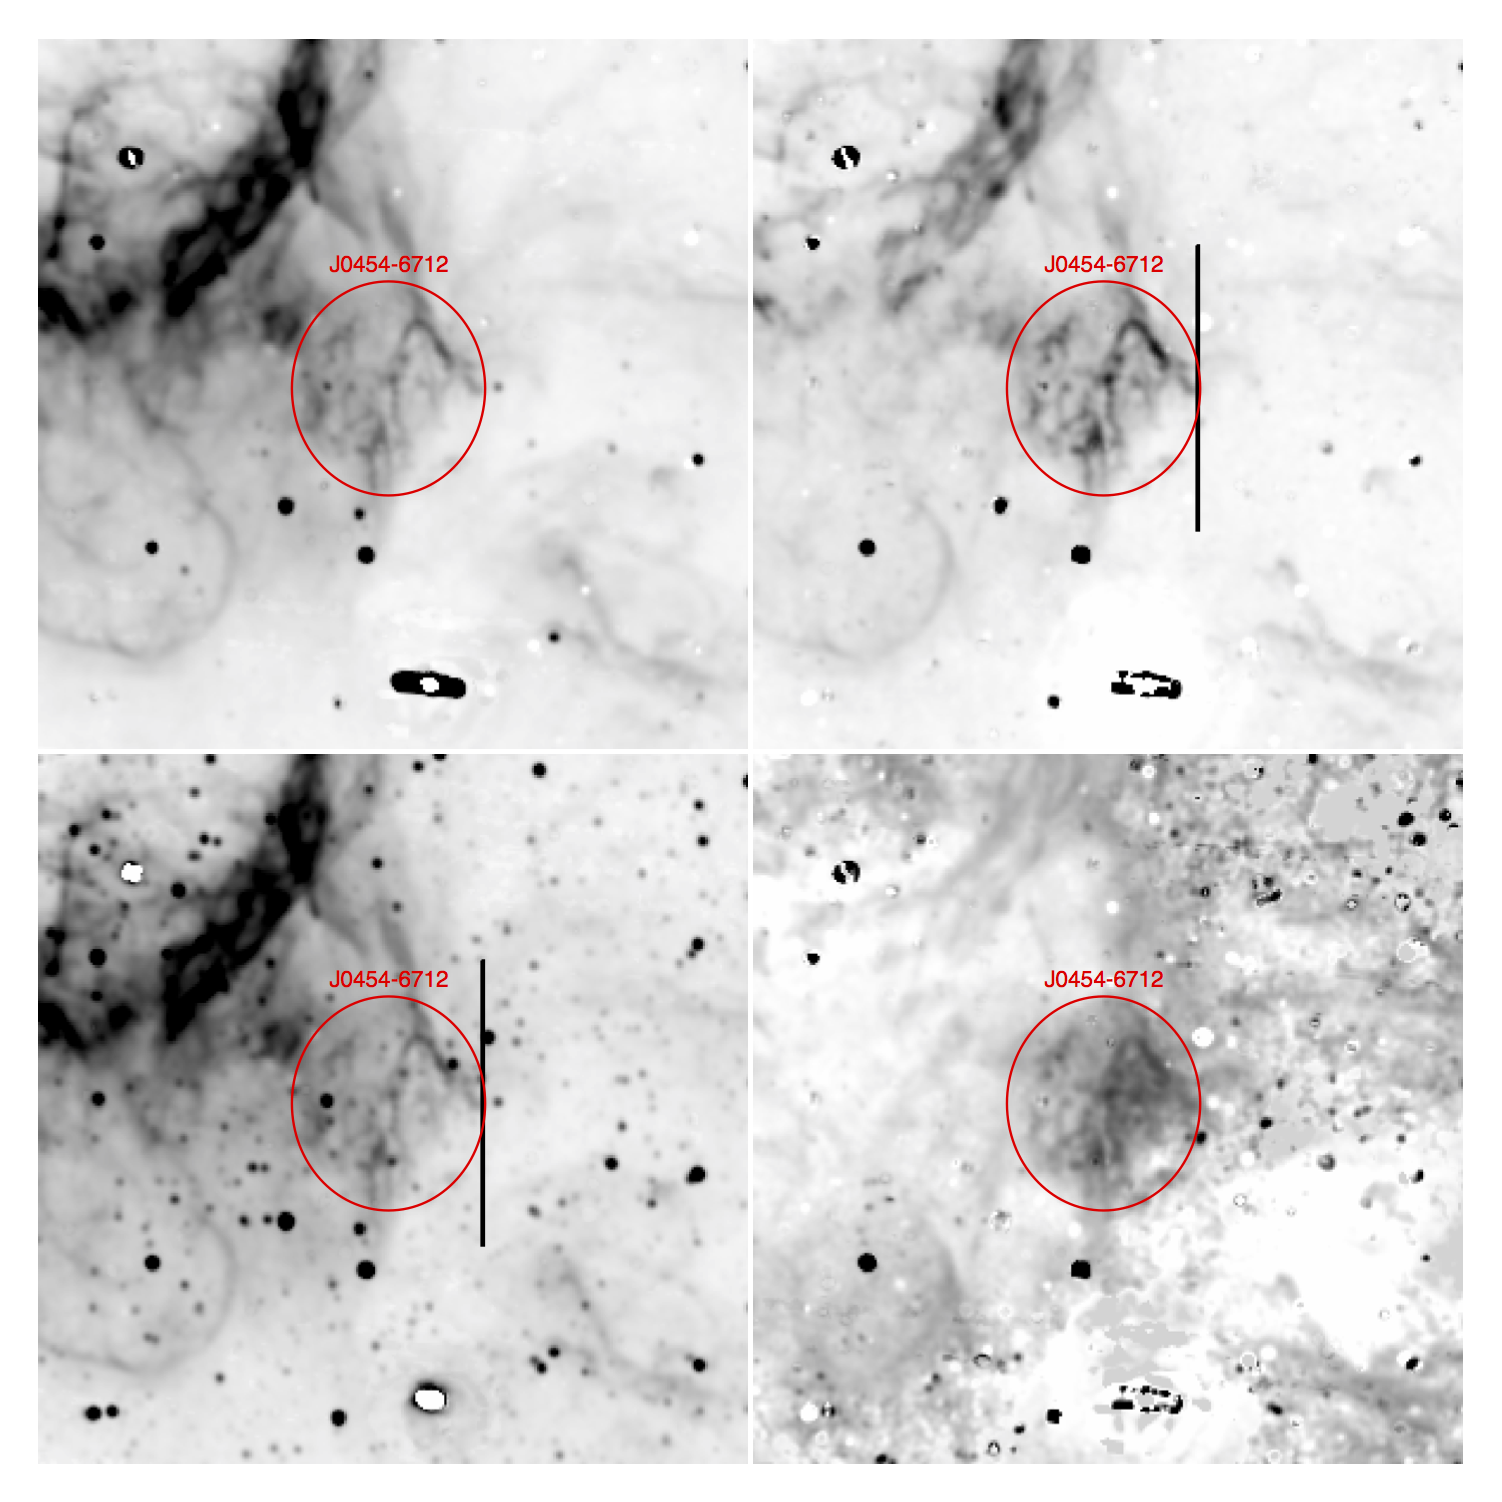
\includegraphics[width=11.cm]{snapshots/J0454-6712.png}
\end{figure}

\newpage
{\bf J0454-6625 = B0454-665 = N11L}

SNR Center:   4:54:49.656   -66:25:40.876     

N-S slit, center on marked star; then offset N 120 arcsec (half of slit length)

Scan:  East  61 arcsec

Scan rate:  122\arcsec/hr for 30 min exposure

Date/Frames:  Night 2, frames 230-232

Exposure Times:  3 x 30 min

\begin{figure}
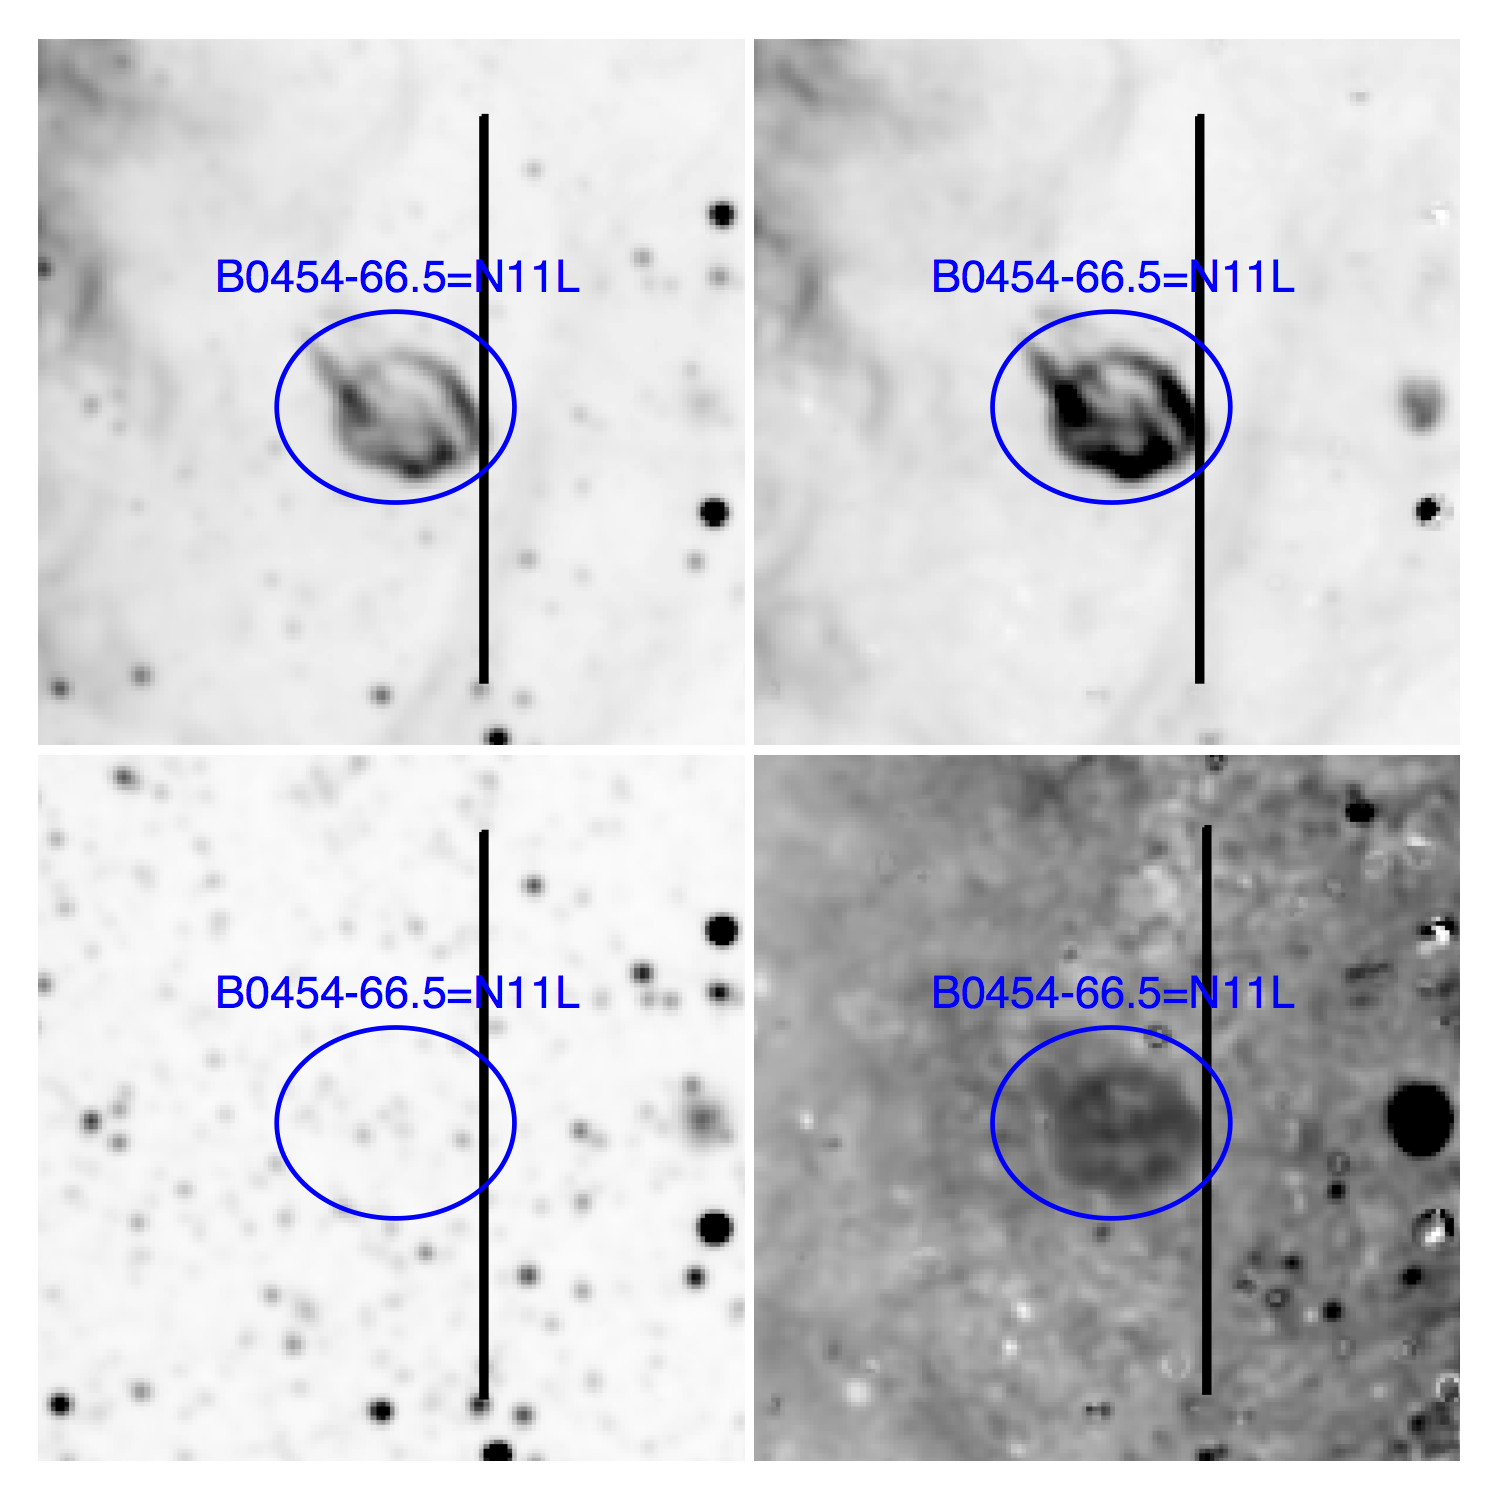
\includegraphics[width=12.5cm]{snapshots/N11L.png}
\end{figure}

\newpage
{\bf J0454-6625 = B0454-665 = N11L\ Longslit (SOAR image)}

SNR Center:   4:54:49.0   -66:25:42.0     

43$^\circ$ slit, center on marked (faint) star; then offset N 4.0\arcsec

Do 2 x 900 s exposures  (if time, do 1000 s, or better 1200 s)

Date/Frames:  

Exposure Times:  

\begin{figure}
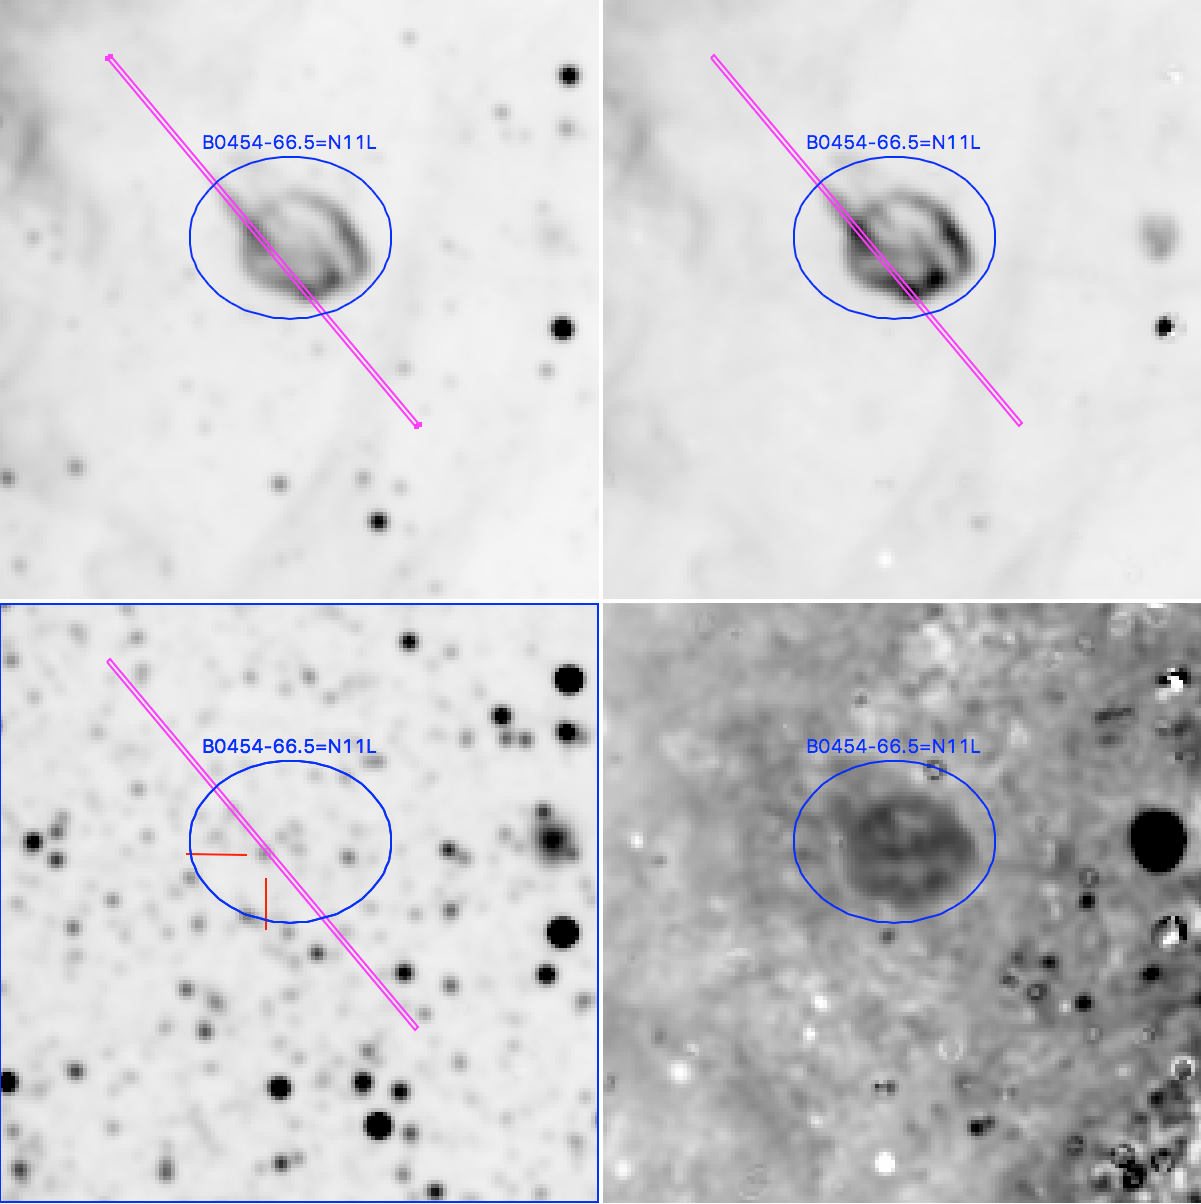
\includegraphics[width=12.5cm]{snapshots/N11L_longslit.png}
\end{figure}

\newpage
{\bf J0455-6839 = B0455-687 = N86}

Slit Center:   4:55:46.302    -68:37:41.817     E-W

center on bright star just N of shell, offset 33\arcsec S, 20\arcsec W

Scan:  South

Scan rate:  400\arcsec/hr

Date/Frames:  Night 1, frames 283-285

Exposure Times:  3 x 30 min

\begin{figure}
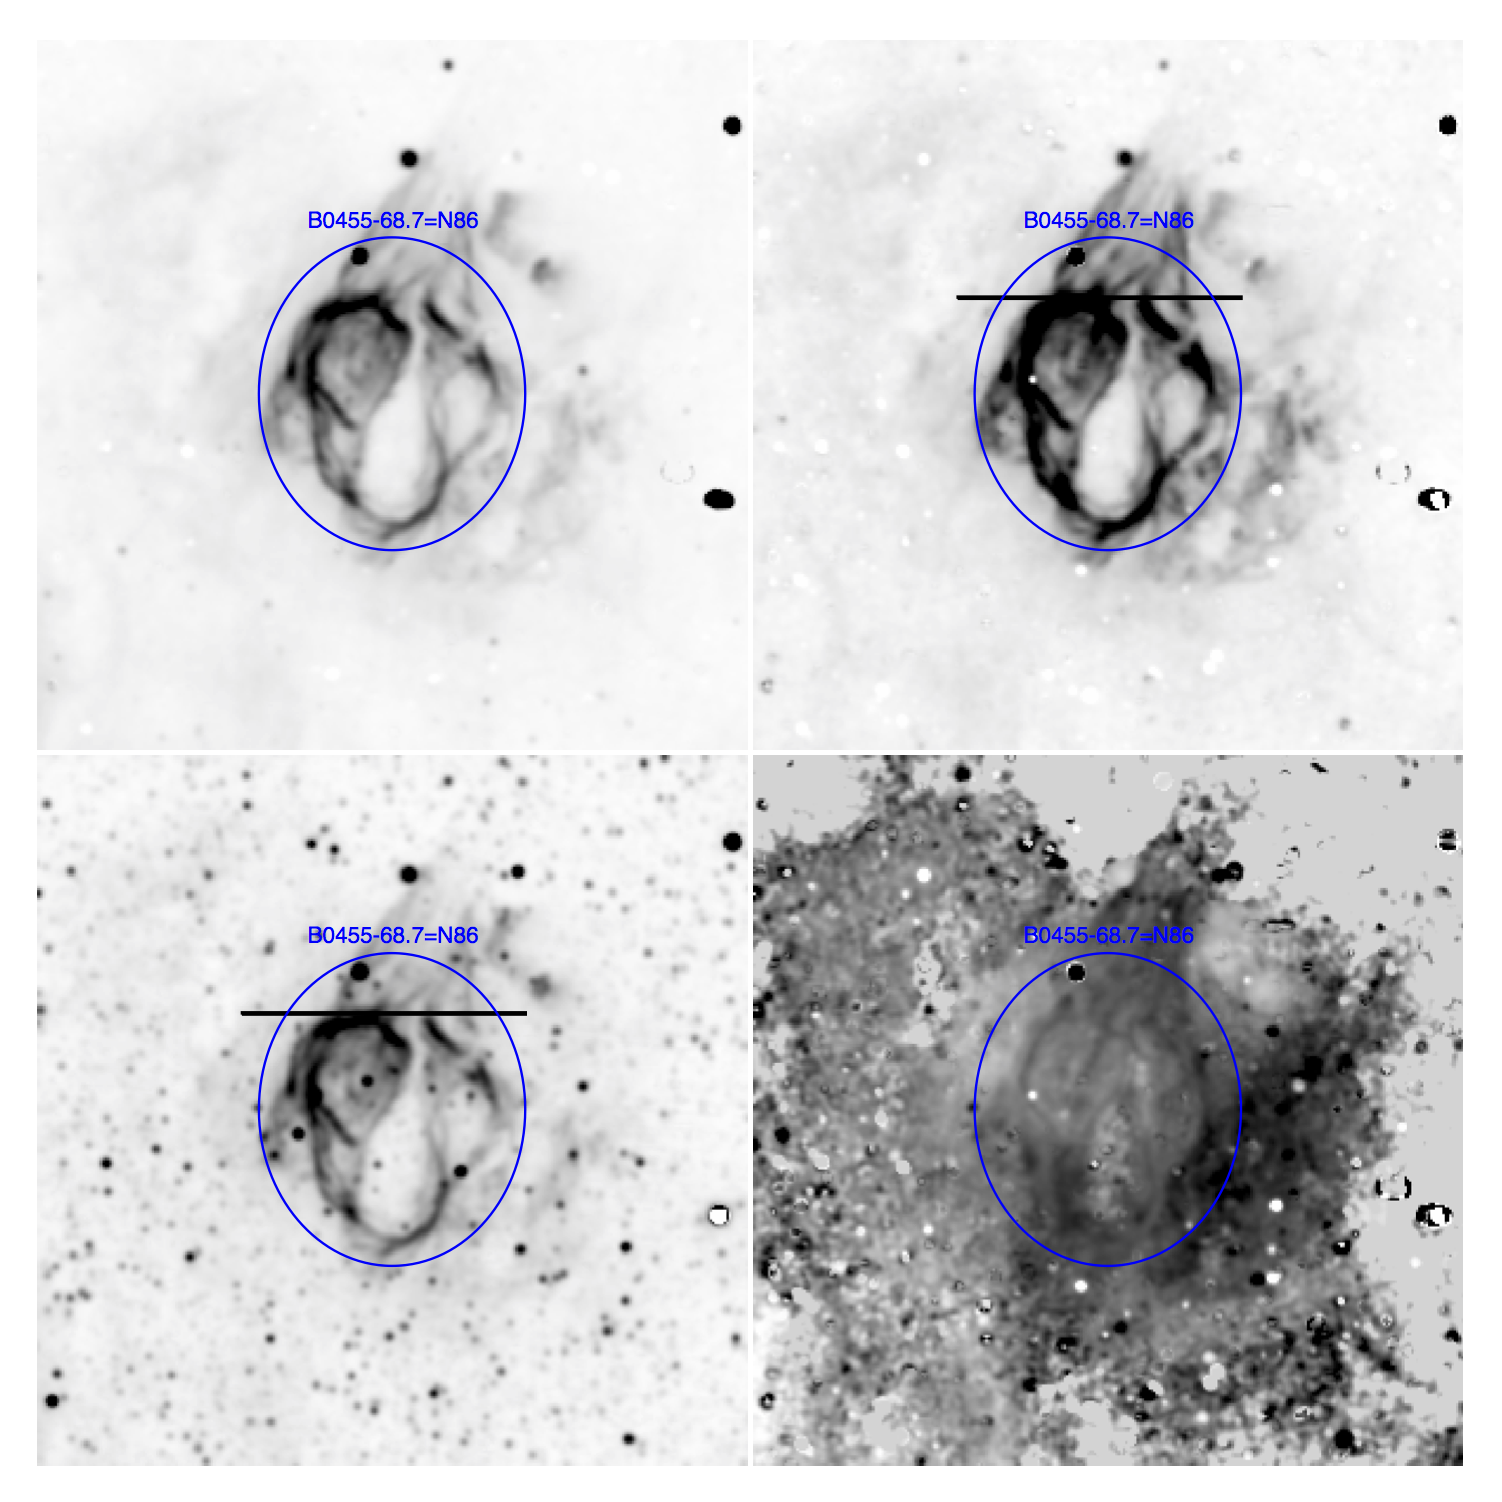
\includegraphics[width=11.cm]{snapshots/B0455-687.png}
\end{figure}

\newpage
{\bf J0455-6839 = B0455-687 = N86 Longslit}

Setup star:   4:55:50    -68:37:09     

Slit P.A. = 74$^\circ$

Offset W 44\arcsec,   S  60.6\arcsec 


Date/Frames:  Night 5, frames:

Exposure Times:  

\begin{figure}
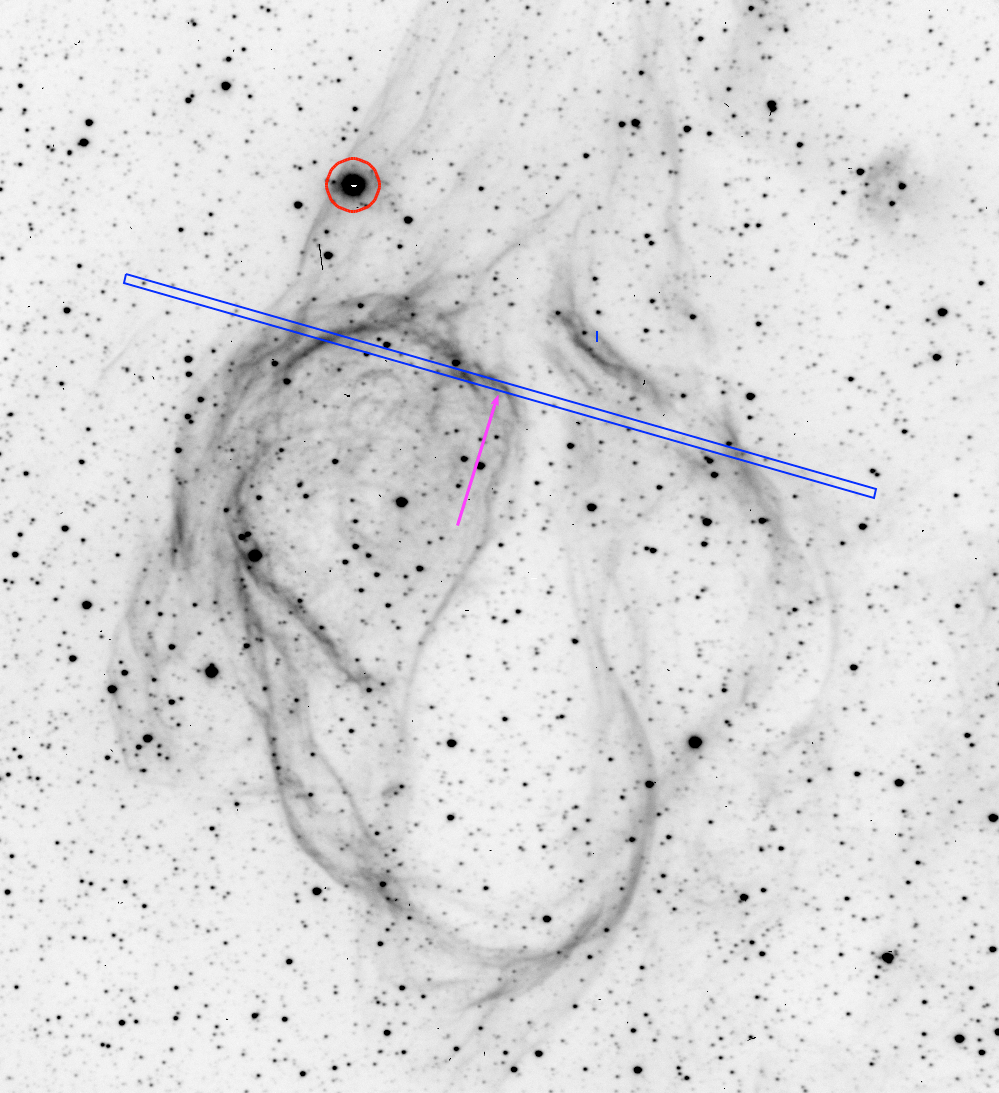
\includegraphics[width=12.5cm]{snapshots/N86_longslit.png}
\end{figure}


\newpage
{\bf J0459-7008 = B0500-702 = N186D}

Slit Center:   4:59:43.935    -70:07:36.307     N-S

Scan:  East

Scan rate:  

Date/Frames:

Exposure Times:  

\begin{figure}
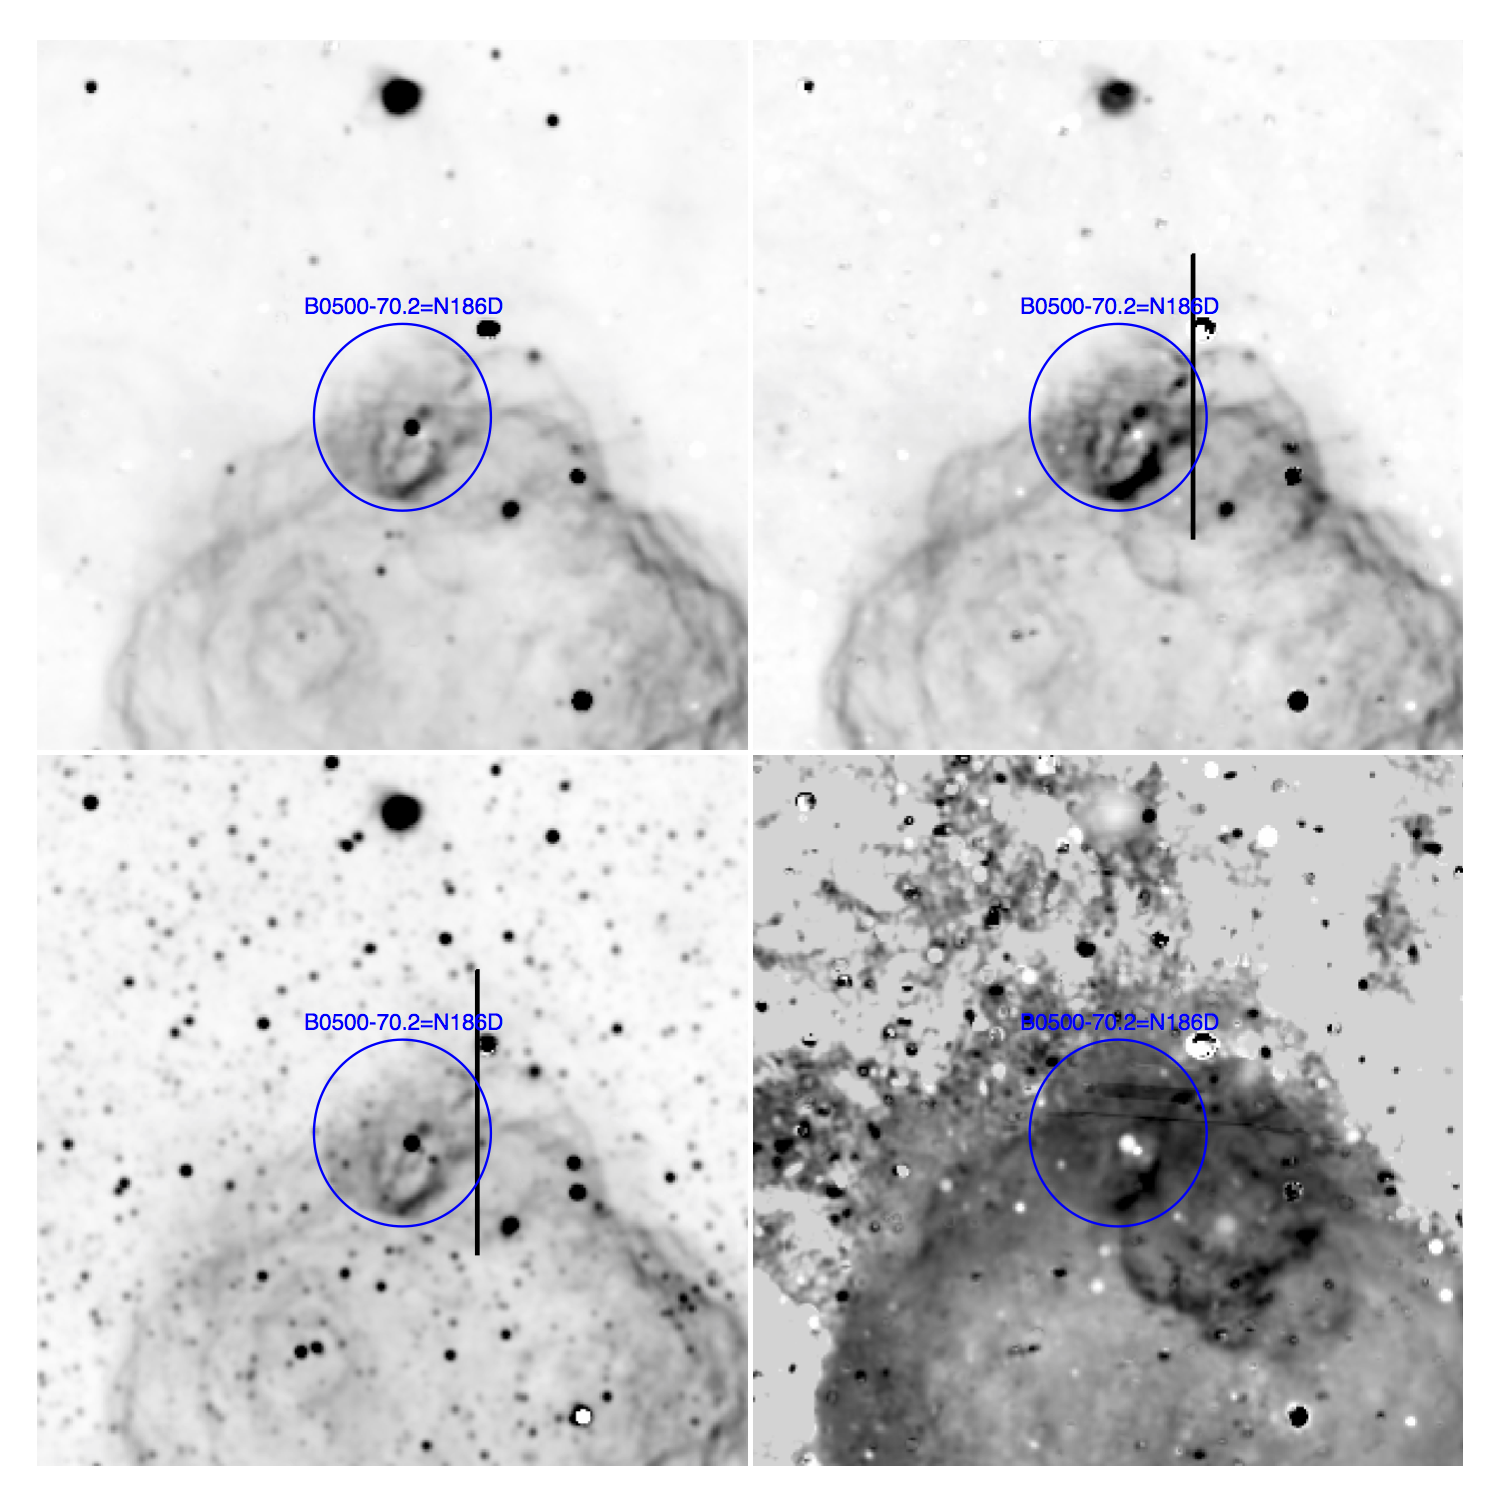
\includegraphics[width=11.cm]{snapshots/B0500-702.png}
\end{figure}

\newpage
{\bf J0505-6752 = B0505-679 = DEML71}  (Balmer-dominated)

Slit Center:   5:05:35.913    -67:52:34.226     N-S

Scan:  East

Scan rate:  

Date/Frames:

Exposure Times:  

\begin{figure}
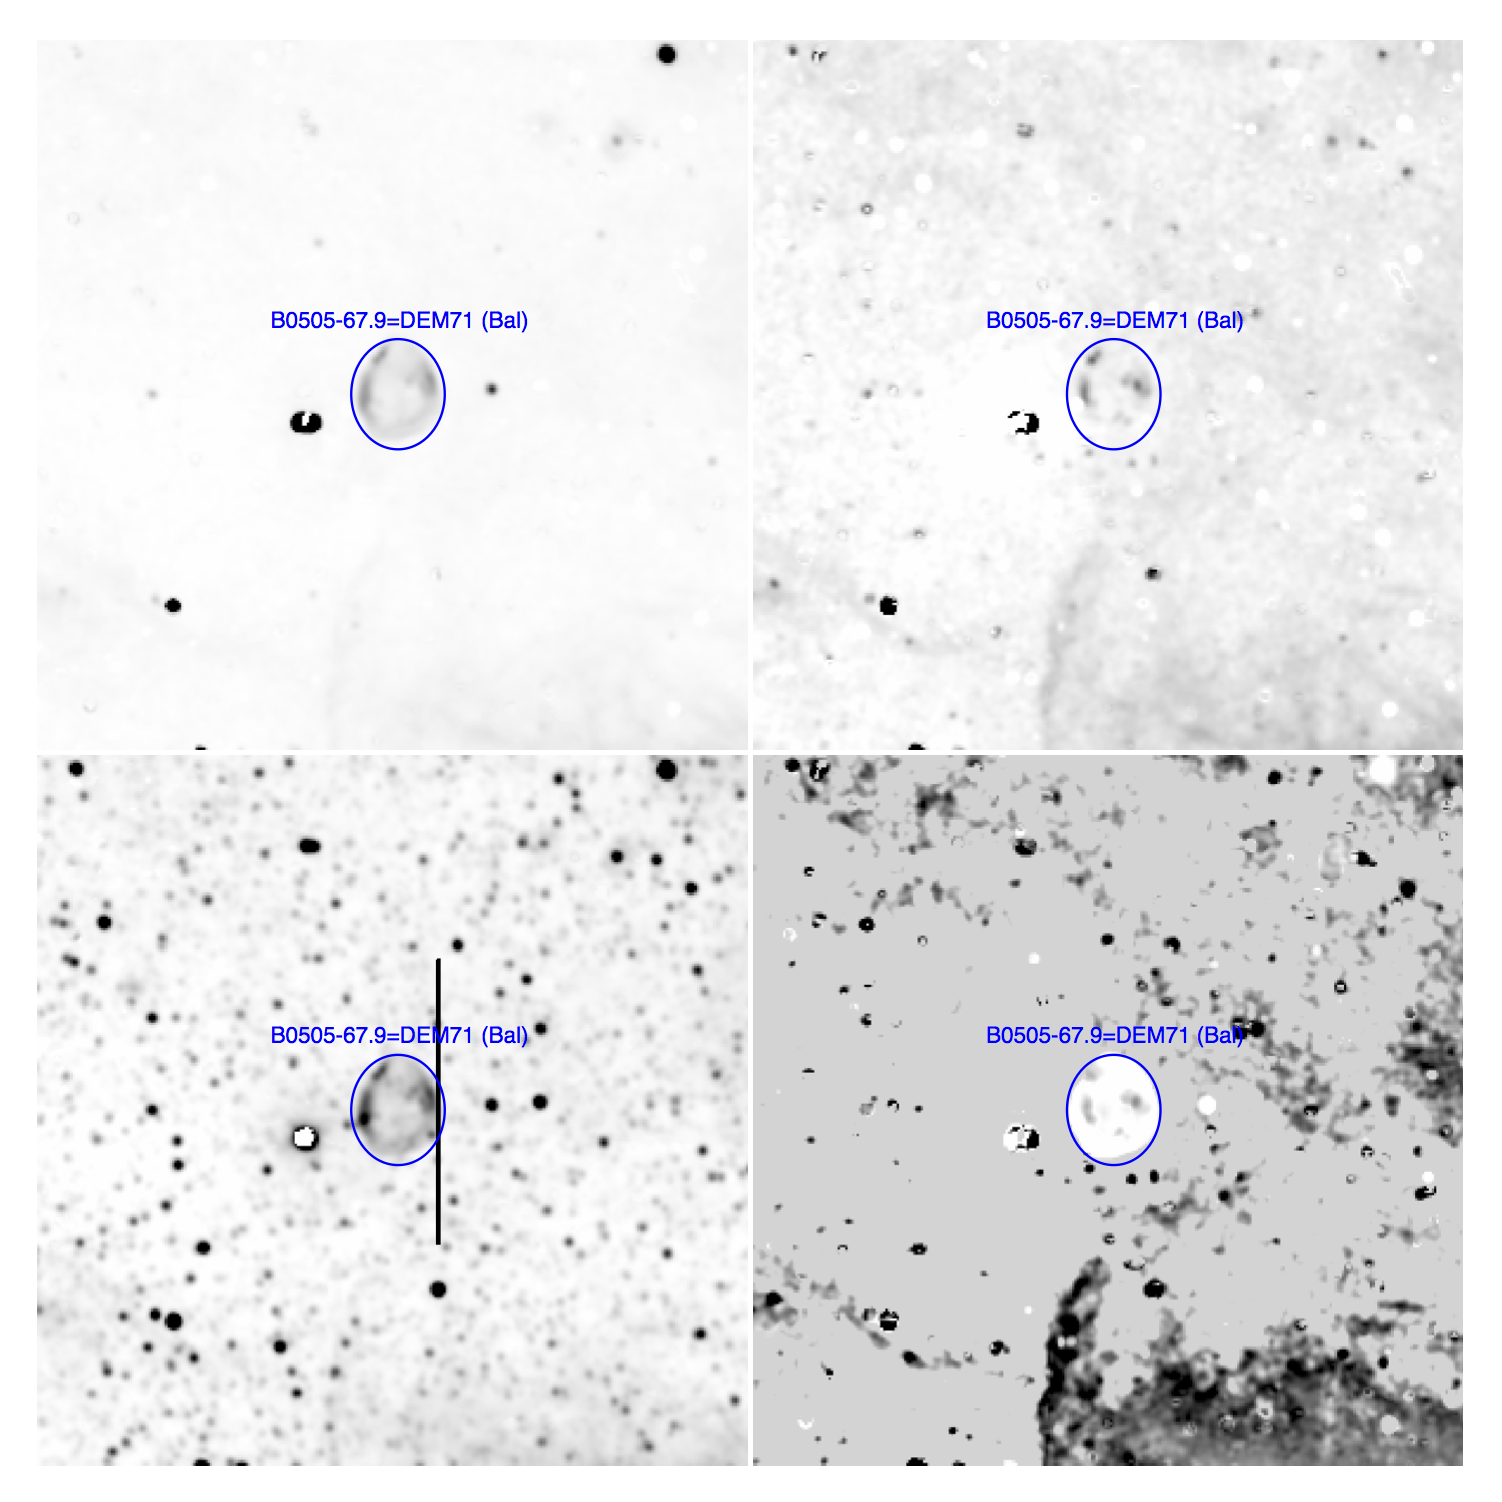
\includegraphics[width=11.cm]{snapshots/B0505-679.png}
\end{figure}

\newpage
{\bf J0505-6801 = B0506-68.0 = N23}  
 
Slit Center:   5:05:46.637    -68:01:47.761     N-S

Scan:  East

Scan rate:  

Date/Frames:

Exposure Times:  

\begin{figure}
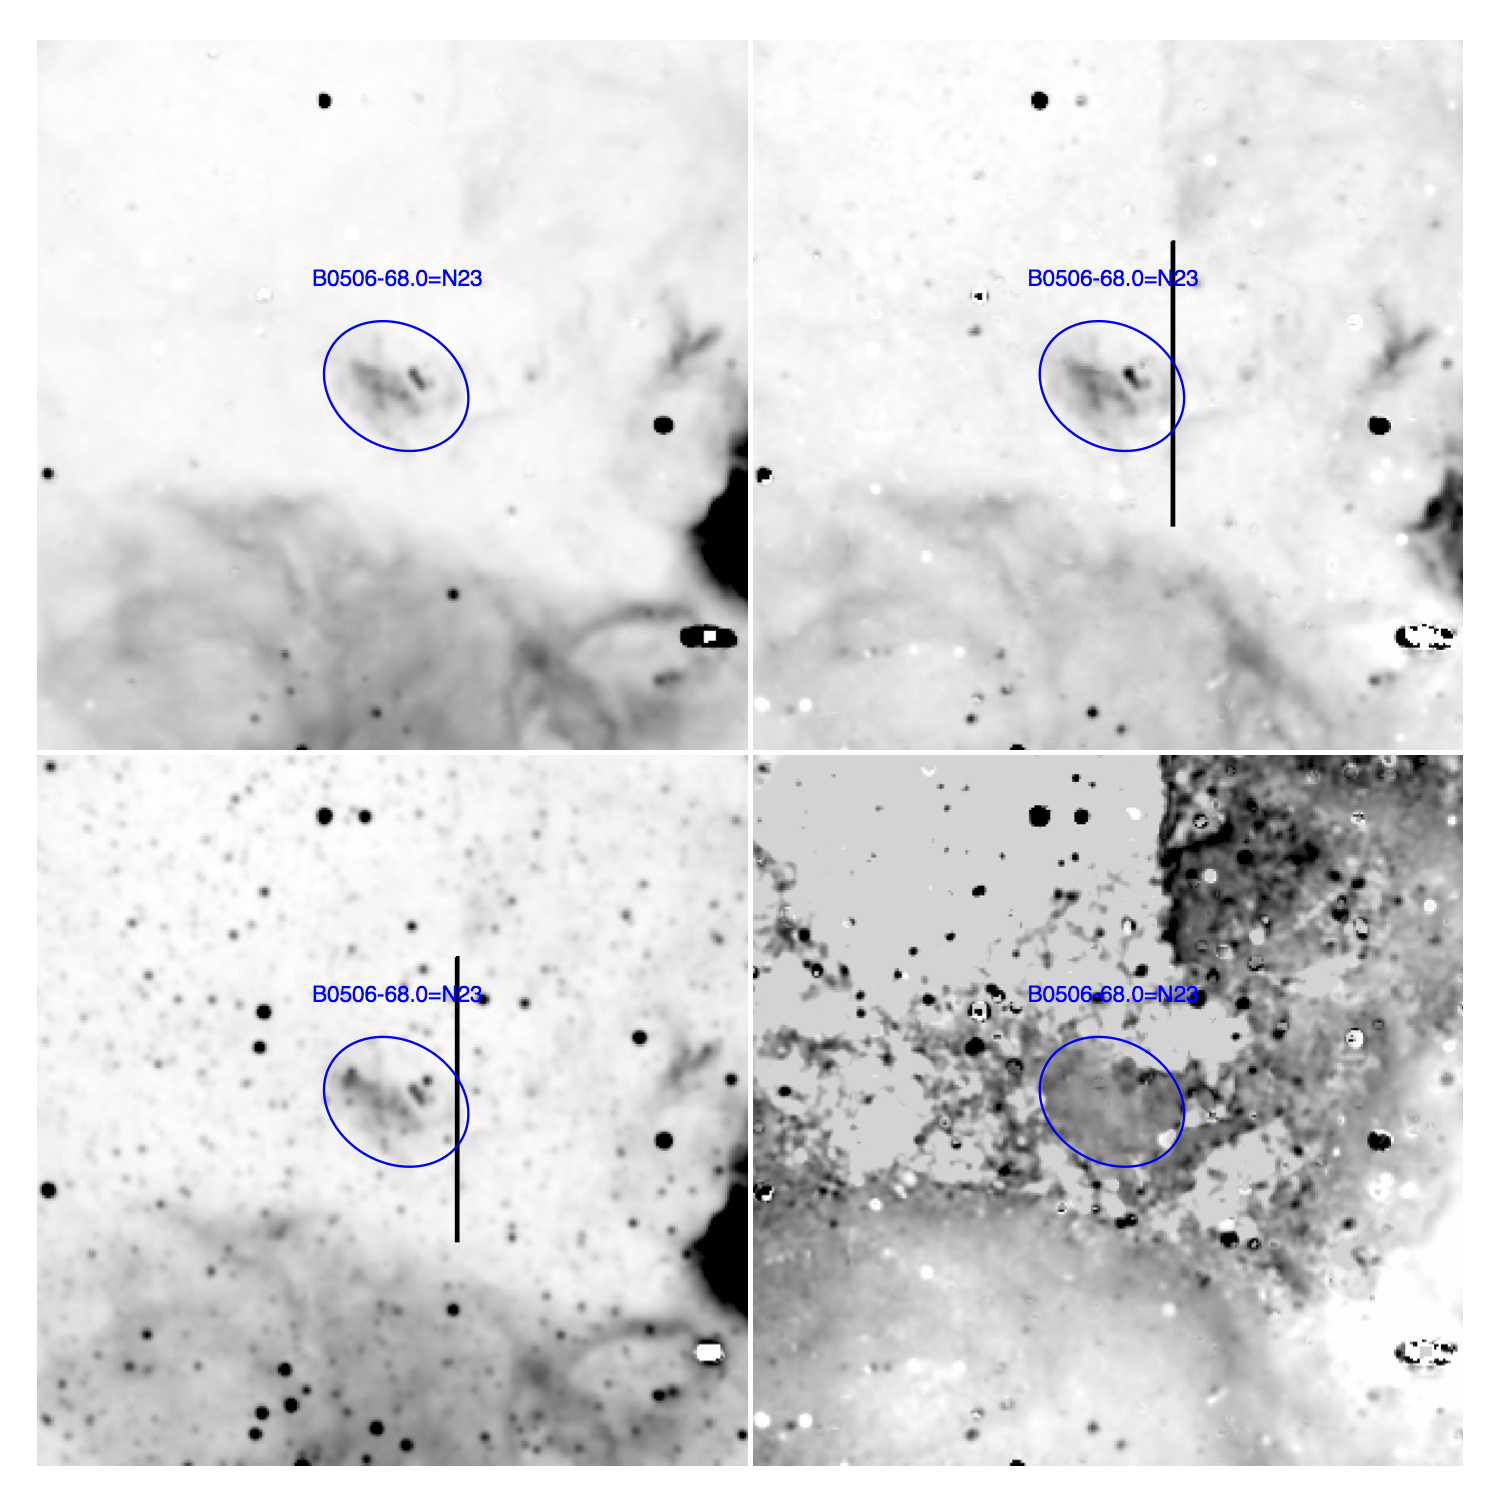
\includegraphics[width=11.cm]{snapshots/B0506-680.png}
\end{figure}

\newpage
{\bf J0506-7025 = DEML80}  
 
Slit Center:   5:06:30.133    -70:25:09.366     N-S

Scan:  East

Scan rate:  

Date/Frames:

Exposure Times:  

\begin{figure}
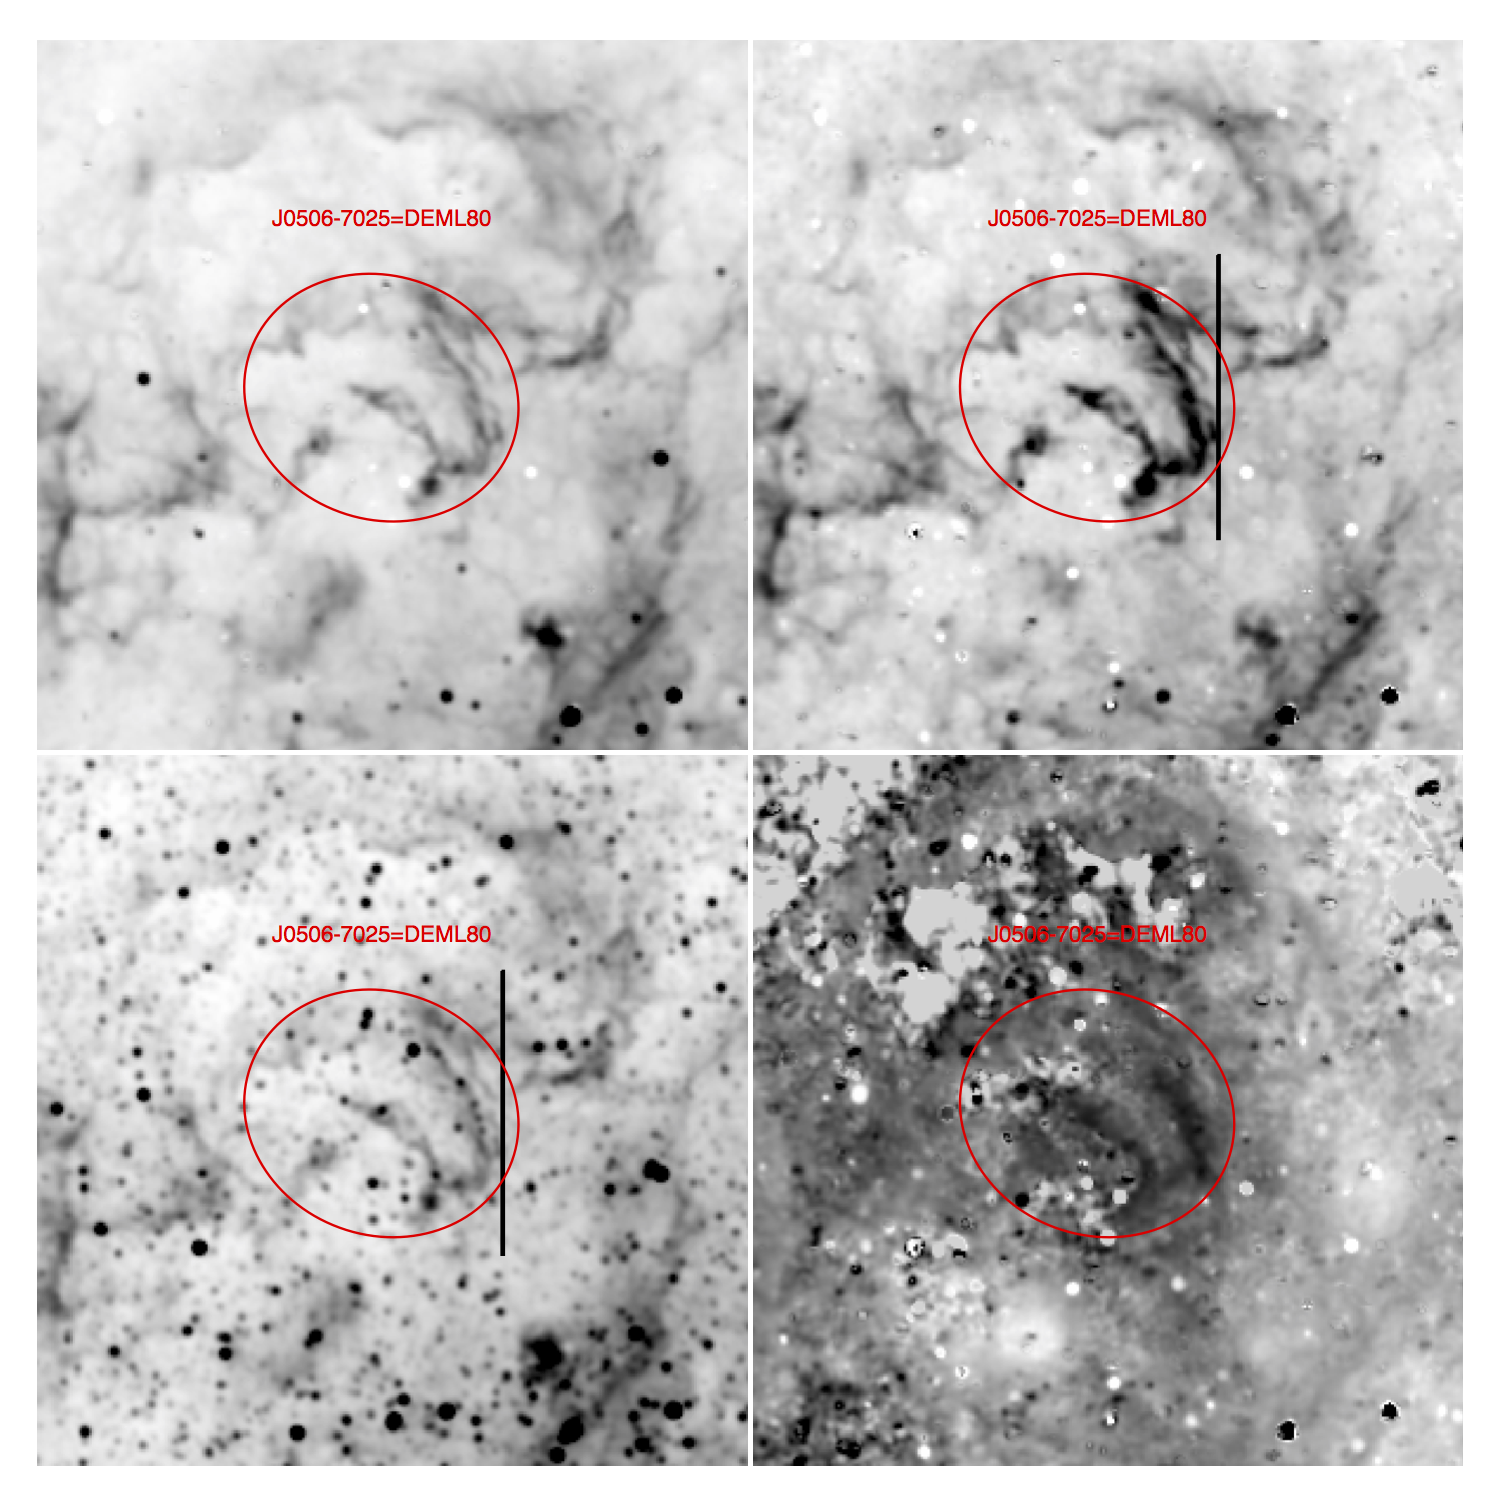
\includegraphics[width=11.cm]{snapshots/J0506-7025.png}
\end{figure}

\newpage
{\bf J0507-7110 new}  
 
Slit Center:   5:07:09.621   -71:10:32.881     N-S

Scan:  East

Scan rate:  

Date/Frames:

Exposure Times:  

\begin{figure}
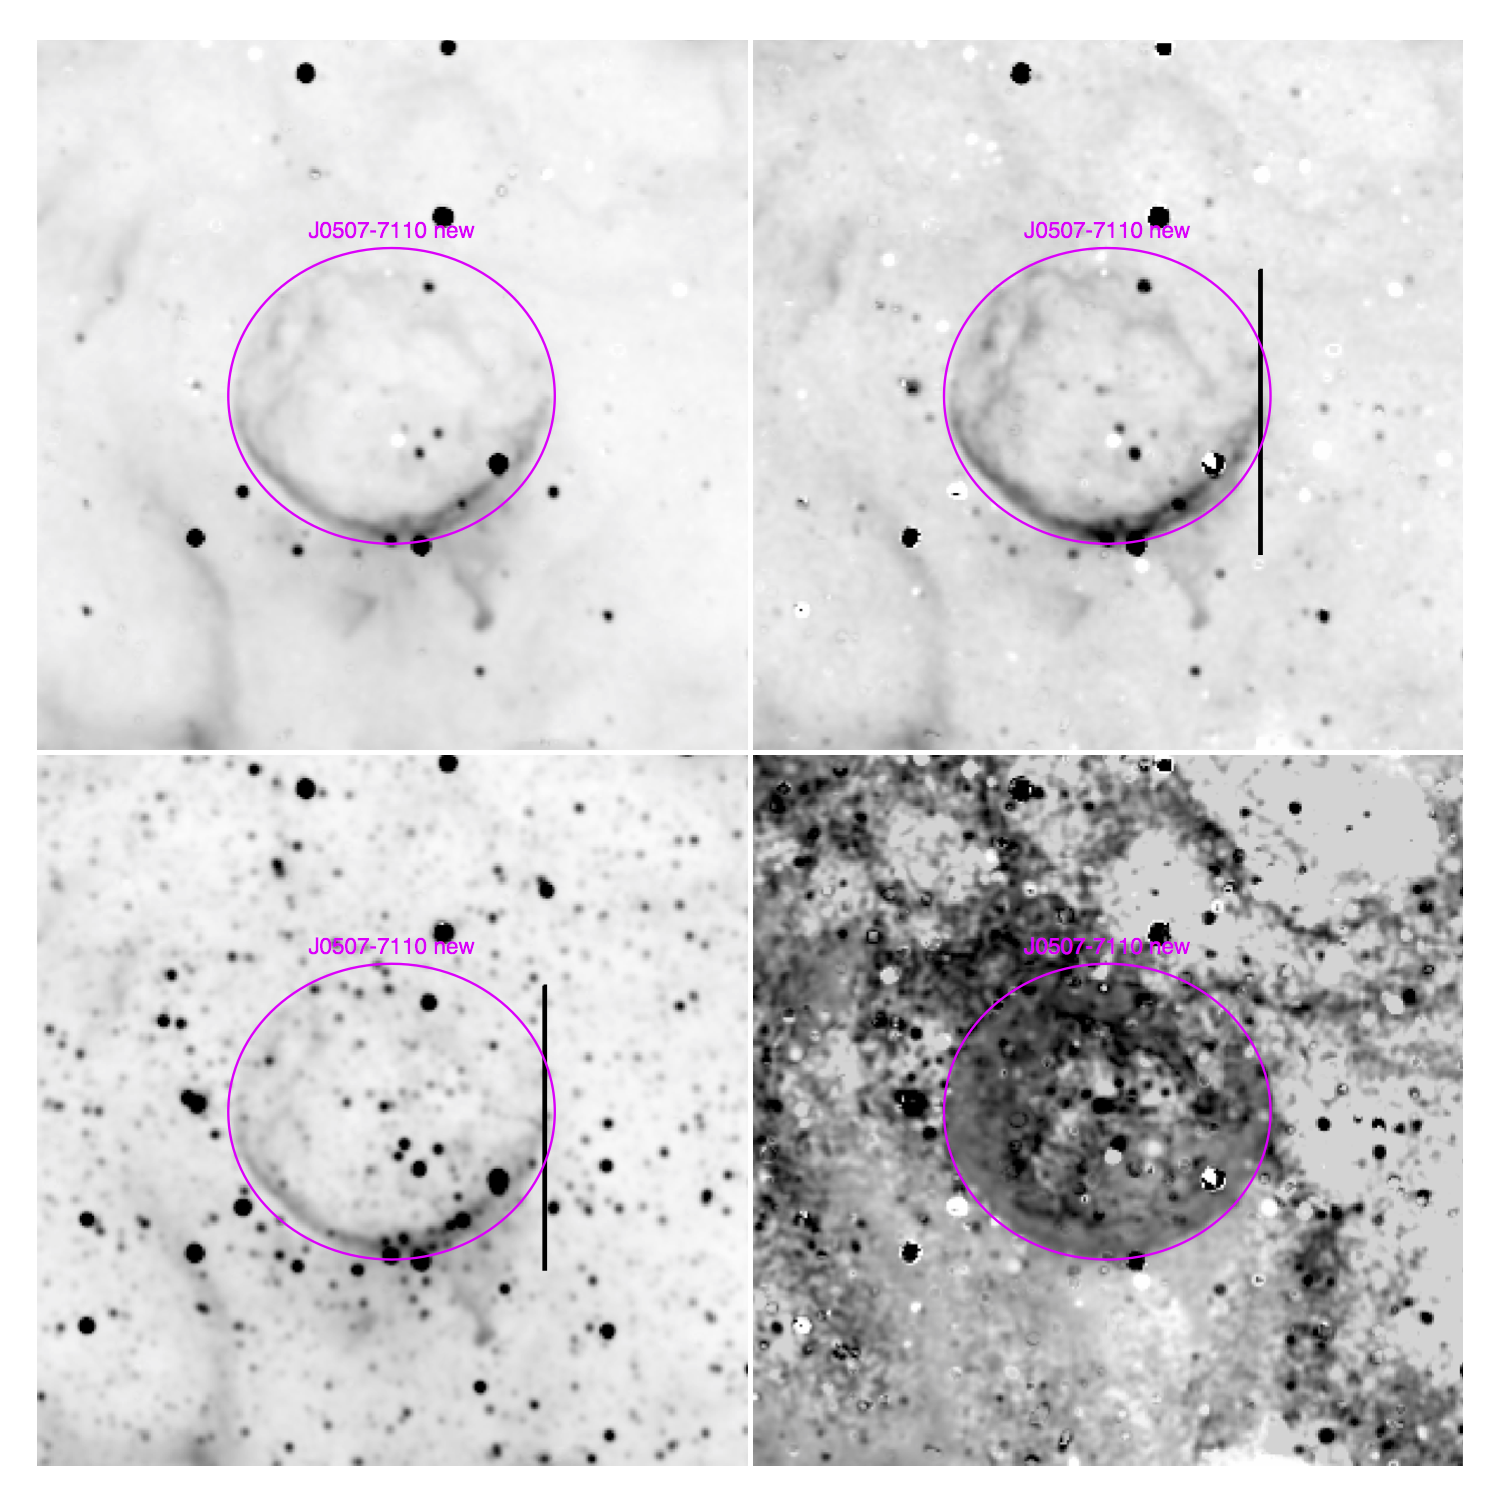
\includegraphics[width=11.cm]{snapshots/J0507-7110.png}
\end{figure}

\newpage
{\bf J0508-6902}  
 
Slit Center:   5:08:26.193   -69:04:07.007     E-W

Scan:  North

Scan rate:  

Date/Frames:

Exposure Times:  

\begin{figure}
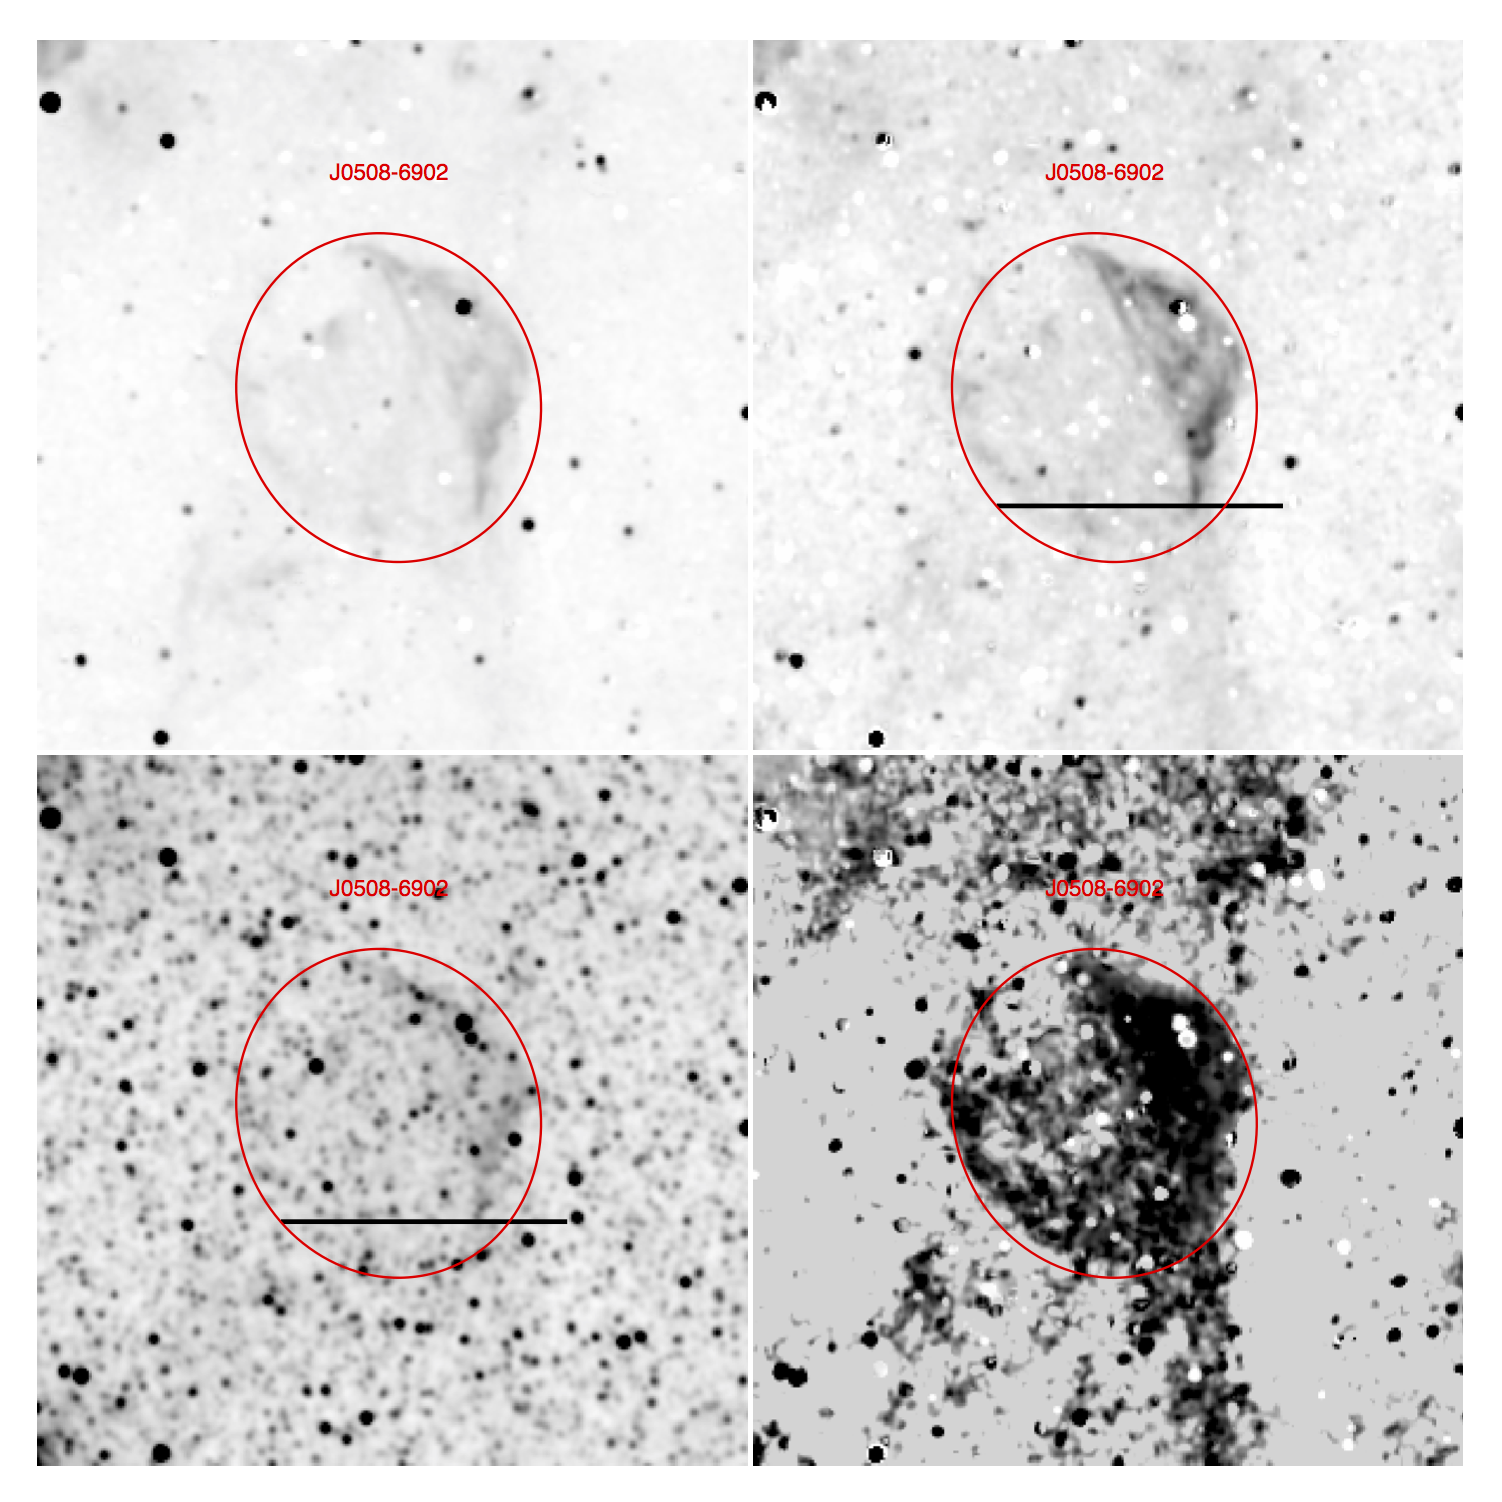
\includegraphics[width=11.cm]{snapshots/J0508-6902.png}
\end{figure}

\newpage
{\bf J508-6843 = B0509-68.7 = N103B}  (Panels $5^\prime$ square)
 
Slit Center:   5:08:57.318   -68:43:28.685     N-S 

Scan:  East, 20\arcsec

Scan rate:   60\arcsec/hr

Date/Frames:  Night 1, frames 292-294

Exposure Times:  

\begin{figure}
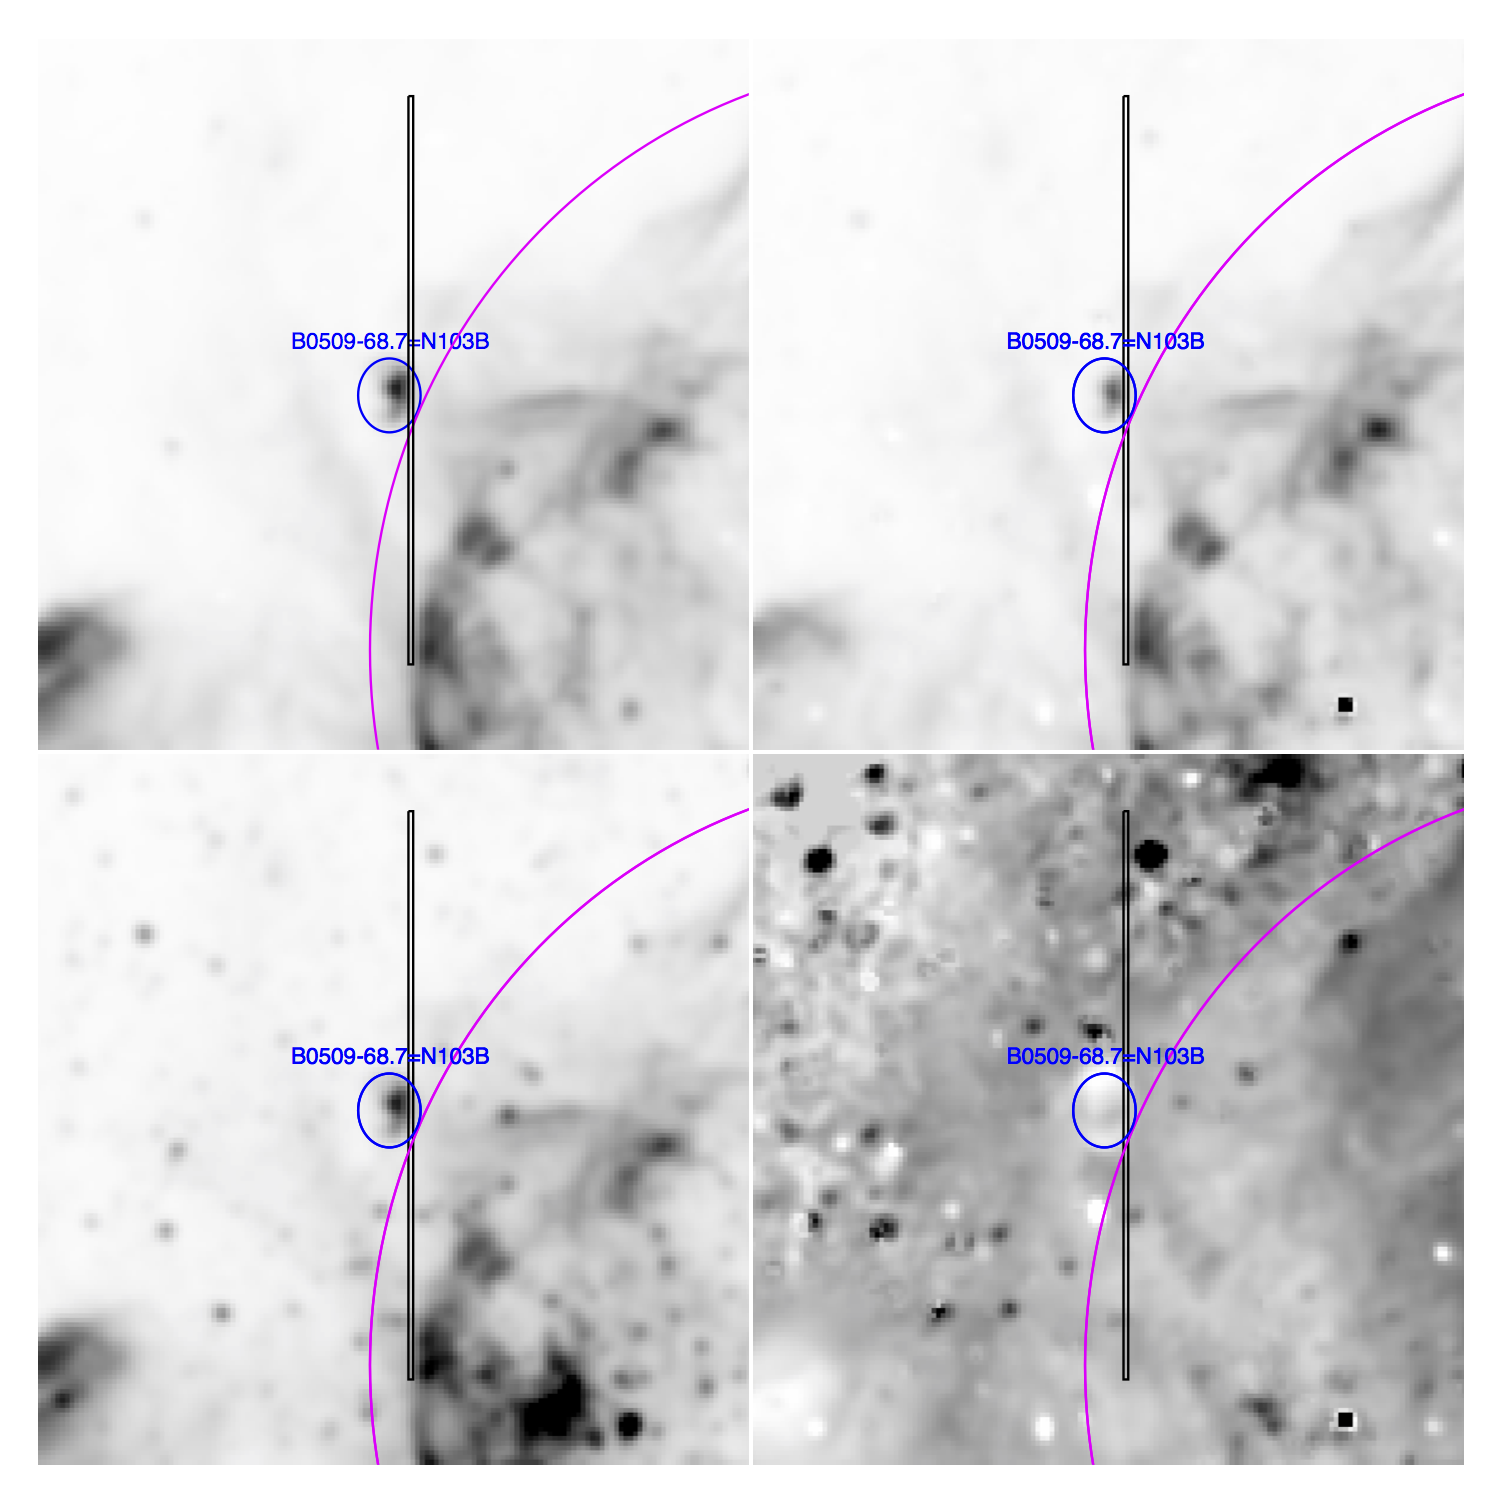
\includegraphics[width=11.cm]{snapshots/N103B_5arcmin.png}
\end{figure}

\newpage
{\bf J509-6731 = B0509-67.5}  (Balmer-dominated; 5 arcmin field)
 
 ($v \approx 6700$ km/s per Hovey 2013, 2015)
 
Slit Center:   5:09:28.212   -67:31:07.856     N-S  

Scan:  East

Scan rate:  

Date/Frames:

Exposure Times:  

\begin{figure}
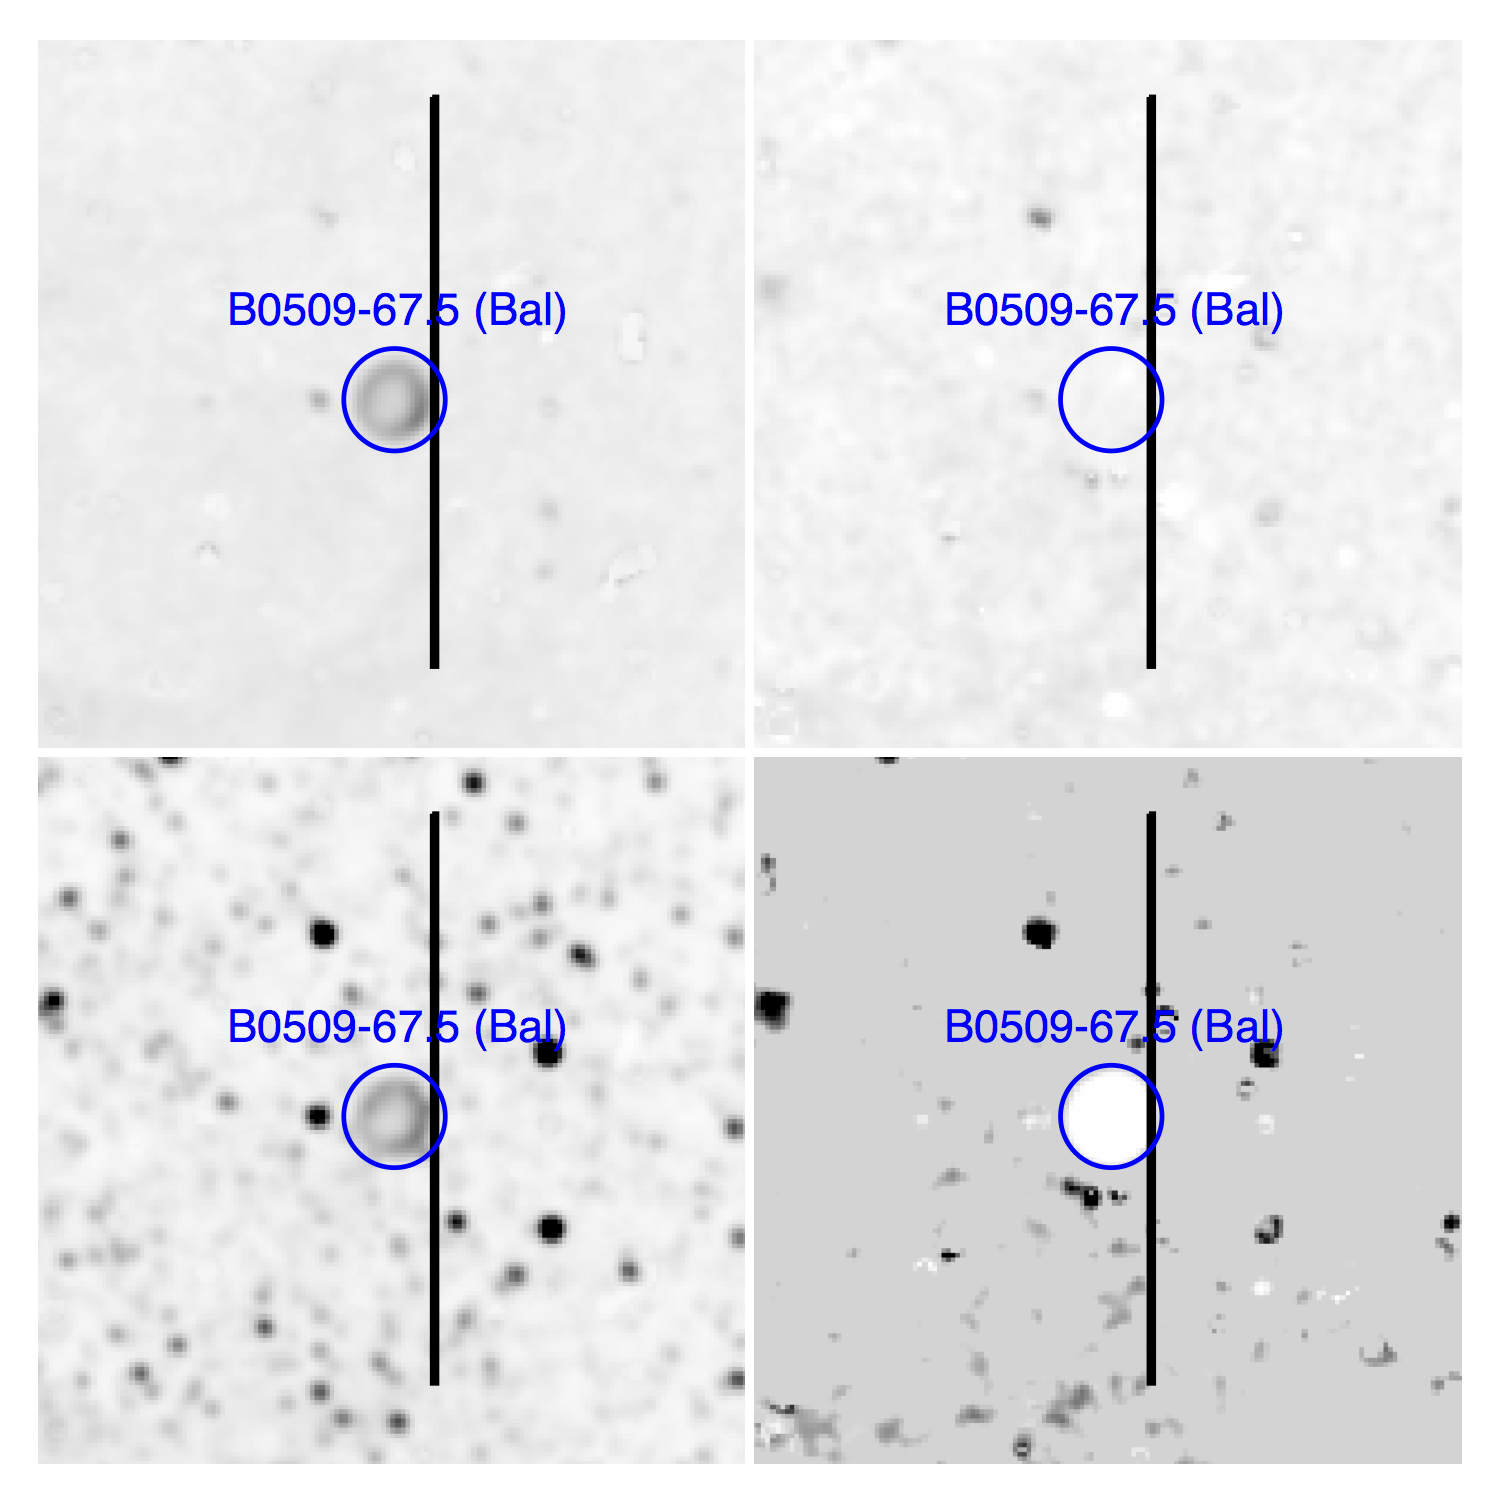
\includegraphics[width=11.cm]{snapshots/B0509-675_5arcmin.png}
\end{figure}

\newpage
{\bf J0511-6759}  
 
Slit Center:   5:10:57.433   -67:59:01.202     N-S 

Scan:  East

Scan rate:  

Date/Frames:

Exposure Times:  

\begin{figure}
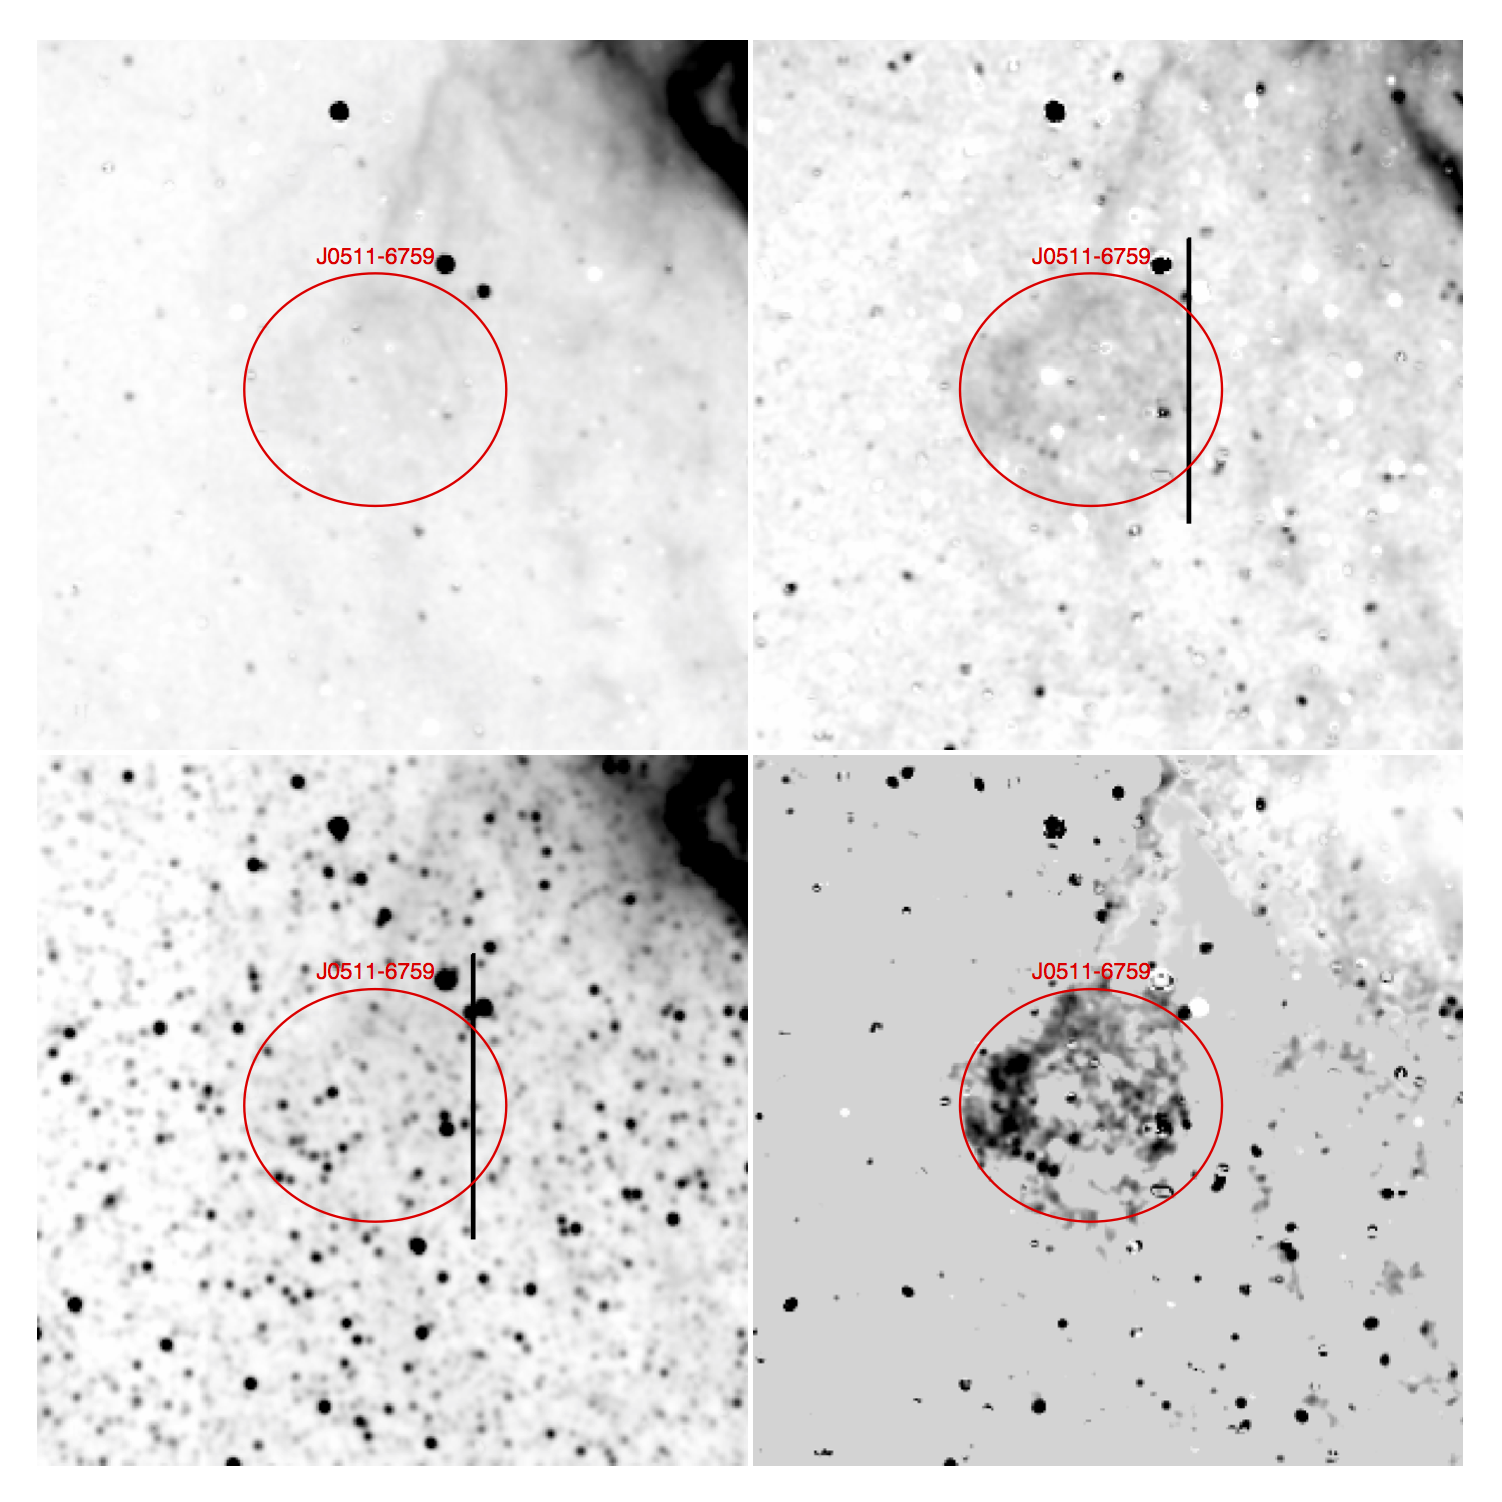
\includegraphics[width=11.cm]{snapshots/J0511-6759.png}
\end{figure}

\newpage
{\bf J0512-6707}  
 
Slit Center:   5:12:25.064  -67:07:04.034    N-S 

Scan:  East

Scan rate:  

Date/Frames:

Exposure Times:  

\begin{figure}
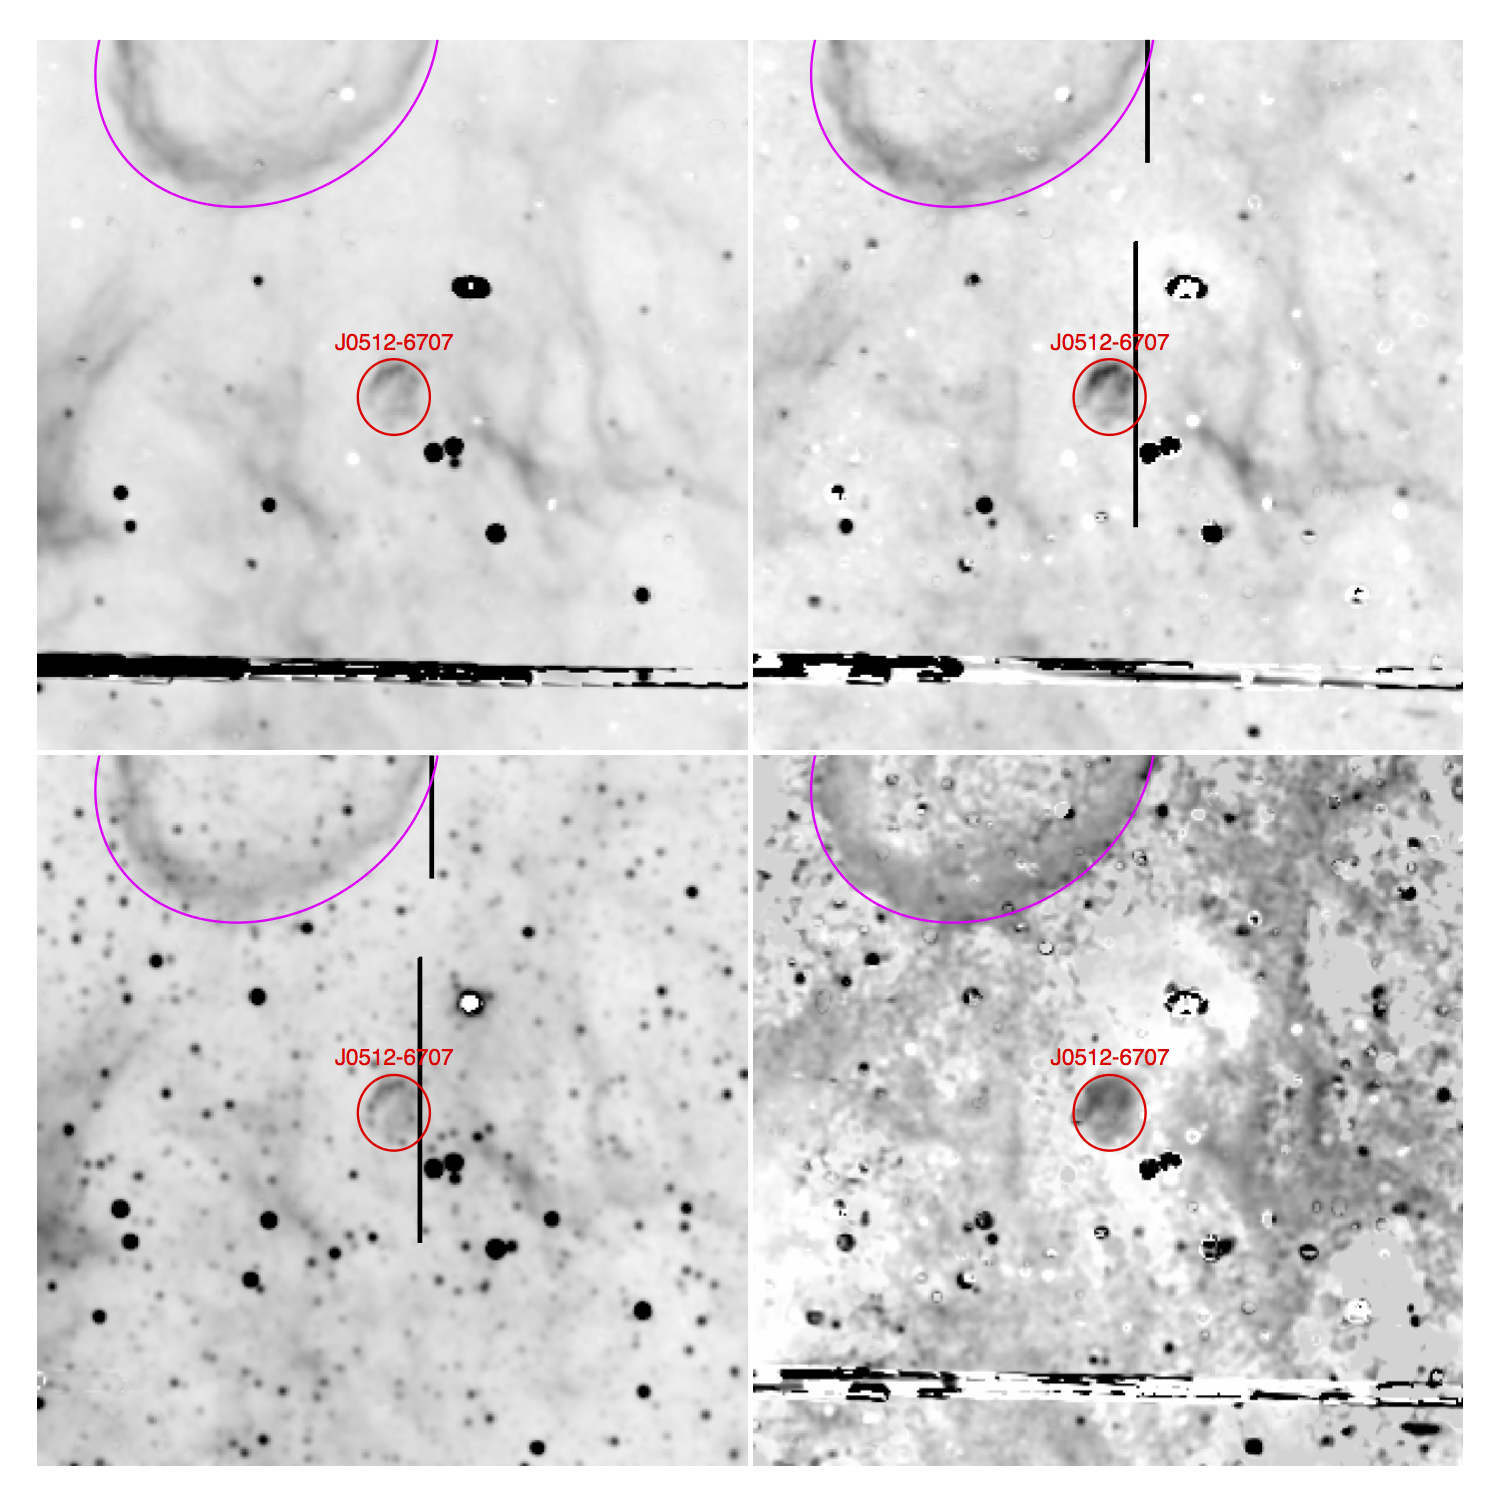
\includegraphics[width=11.cm]{snapshots/J0512-6707.png}
\end{figure}

\newpage
{\bf J0512-6702 (new)}  
 
Slit Center:   5:10:57.433   -67:59:01.202    N-S 

Scan:  East

Scan rate:  

Date/Frames:

Exposure Times:  

\begin{figure}
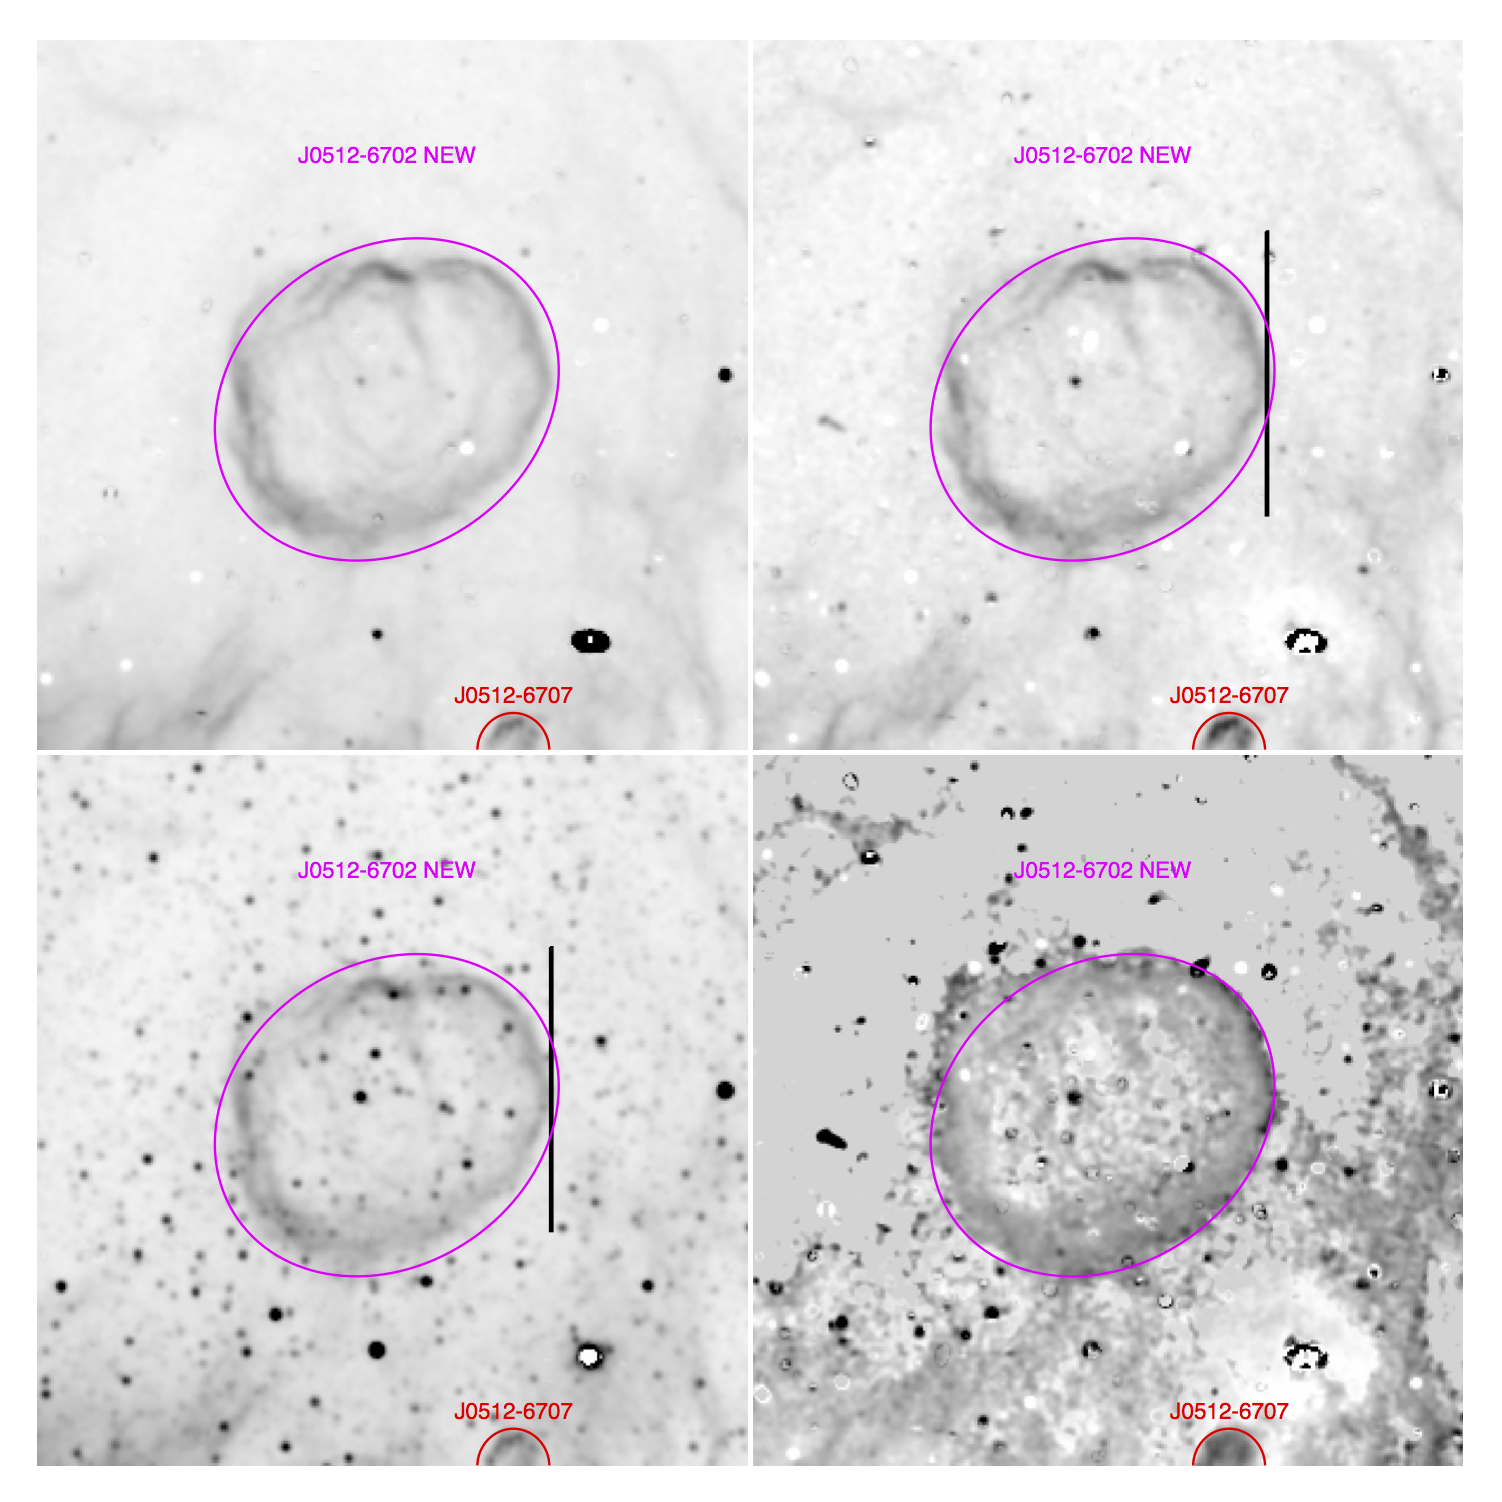
\includegraphics[width=11.cm]{snapshots/J0512-6702.png}
\end{figure}

\newpage
{\bf J0513-6912-6912 = B0513-69.2}  
 
Slit Center:   5:12:53.465, -69:12:15.860    N-S 

Scan:  East

Scan rate:  

Date/Frames:

Exposure Times:  

\begin{figure}
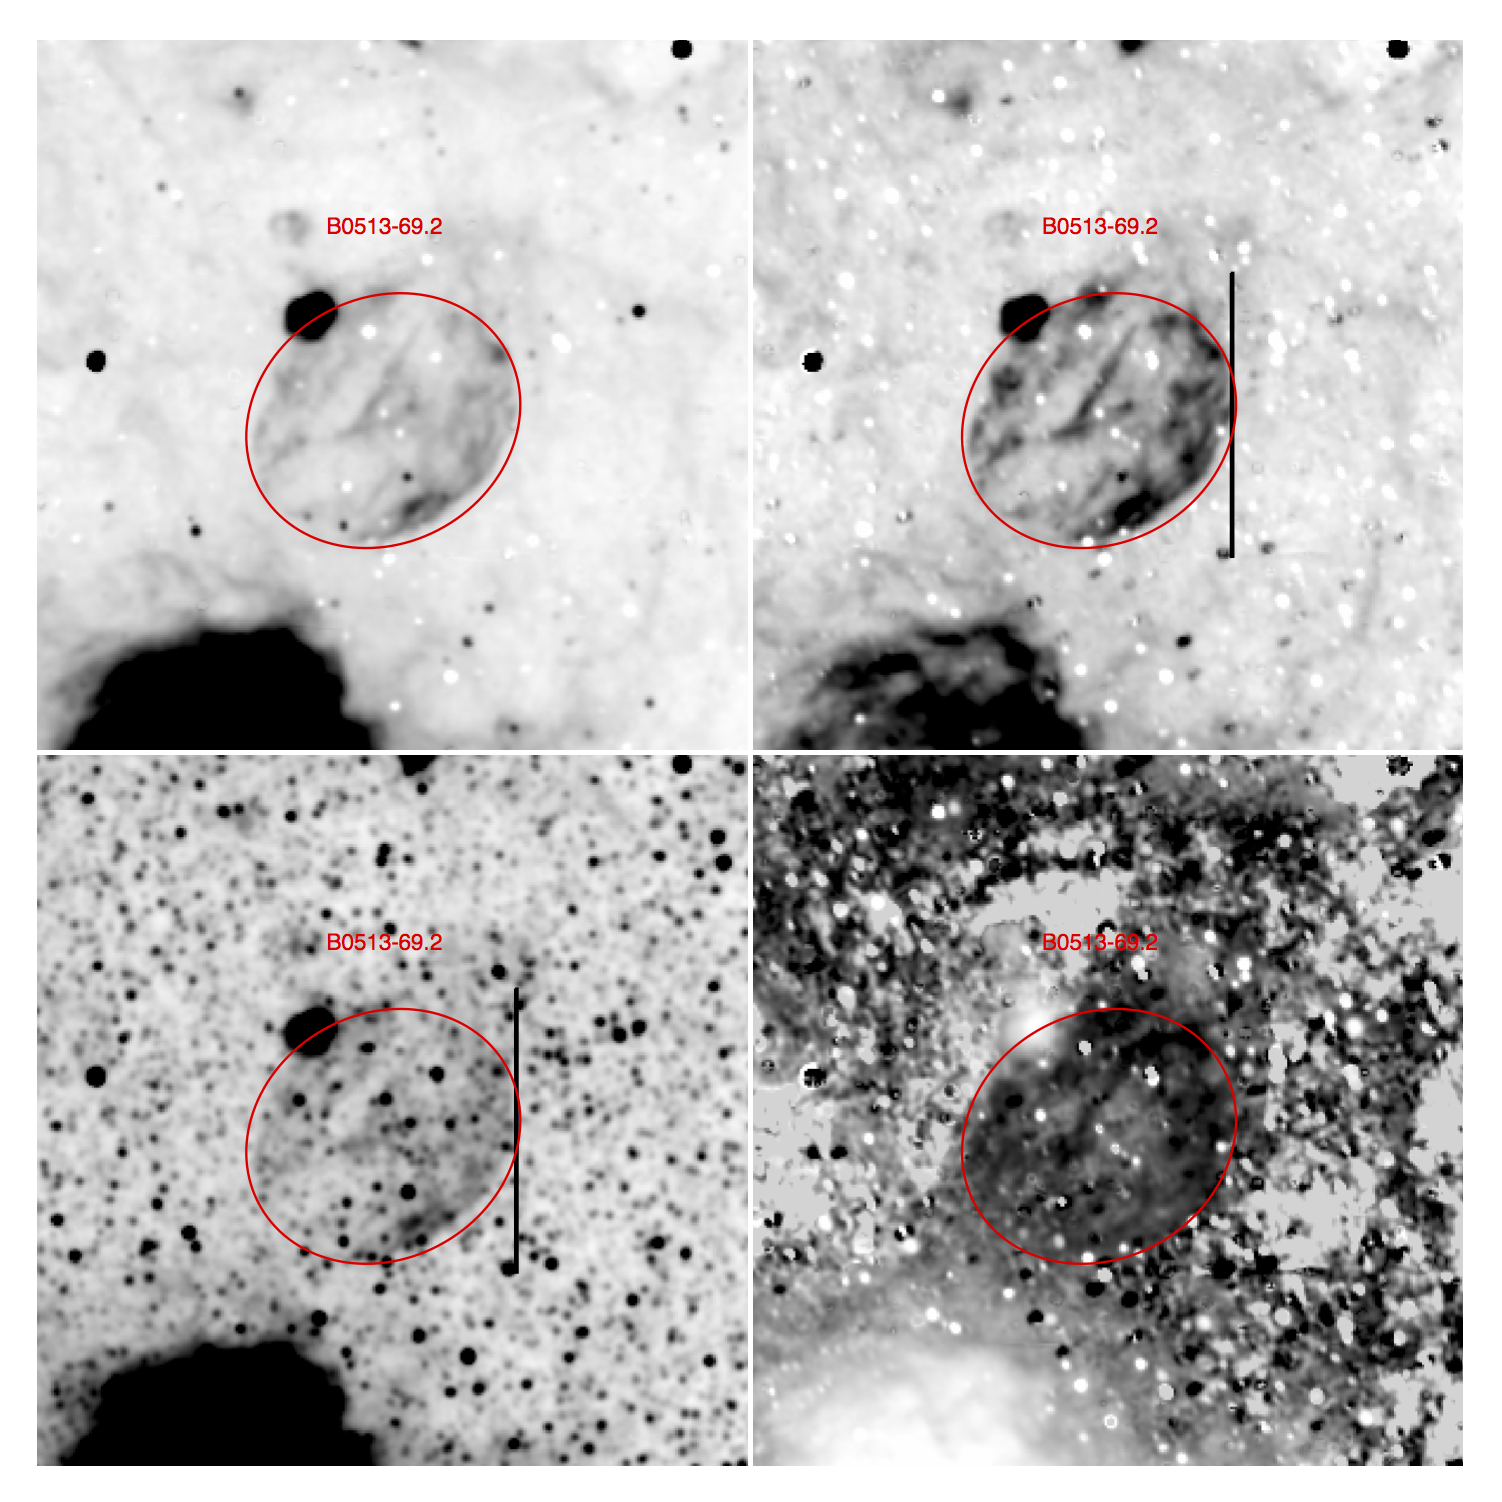
\includegraphics[width=11.cm]{snapshots/B0513-692.png}
\end{figure}

\newpage
{\bf J0514-6840}  
 
Slit Center:   5:14:01.698 -68:40:53.008    N-S 

Scan:  East

Scan rate:  

Date/Frames:

Exposure Times:  

\begin{figure}
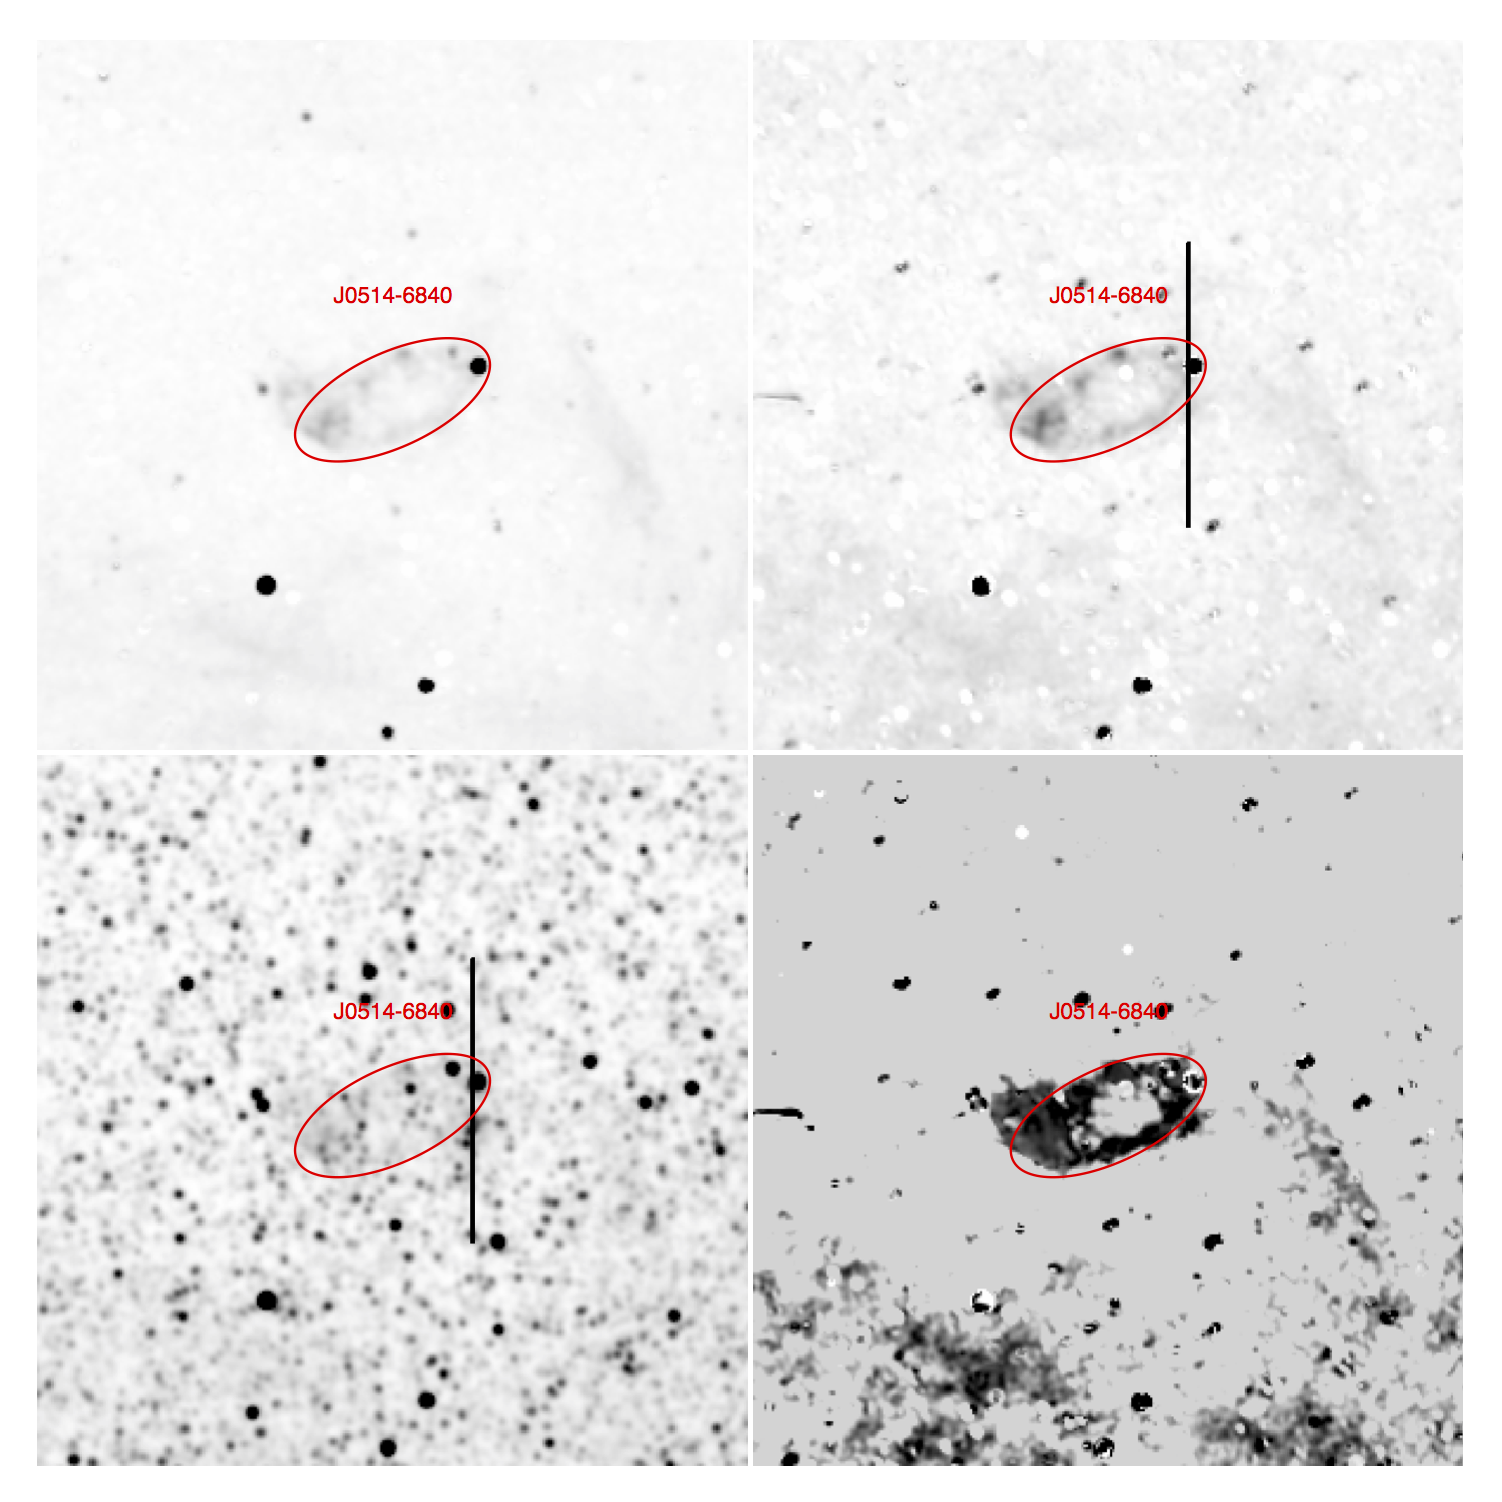
\includegraphics[width=11.cm]{snapshots/J0514-6840.png}
\end{figure}

\newpage
{\bf J0517-6759}  
 
Slit Center:   5:17:07.268 -68:01:28.513    E-W 

Scan:  North

Scan rate:  

Date/Frames:

Exposure Times:  

\begin{figure}
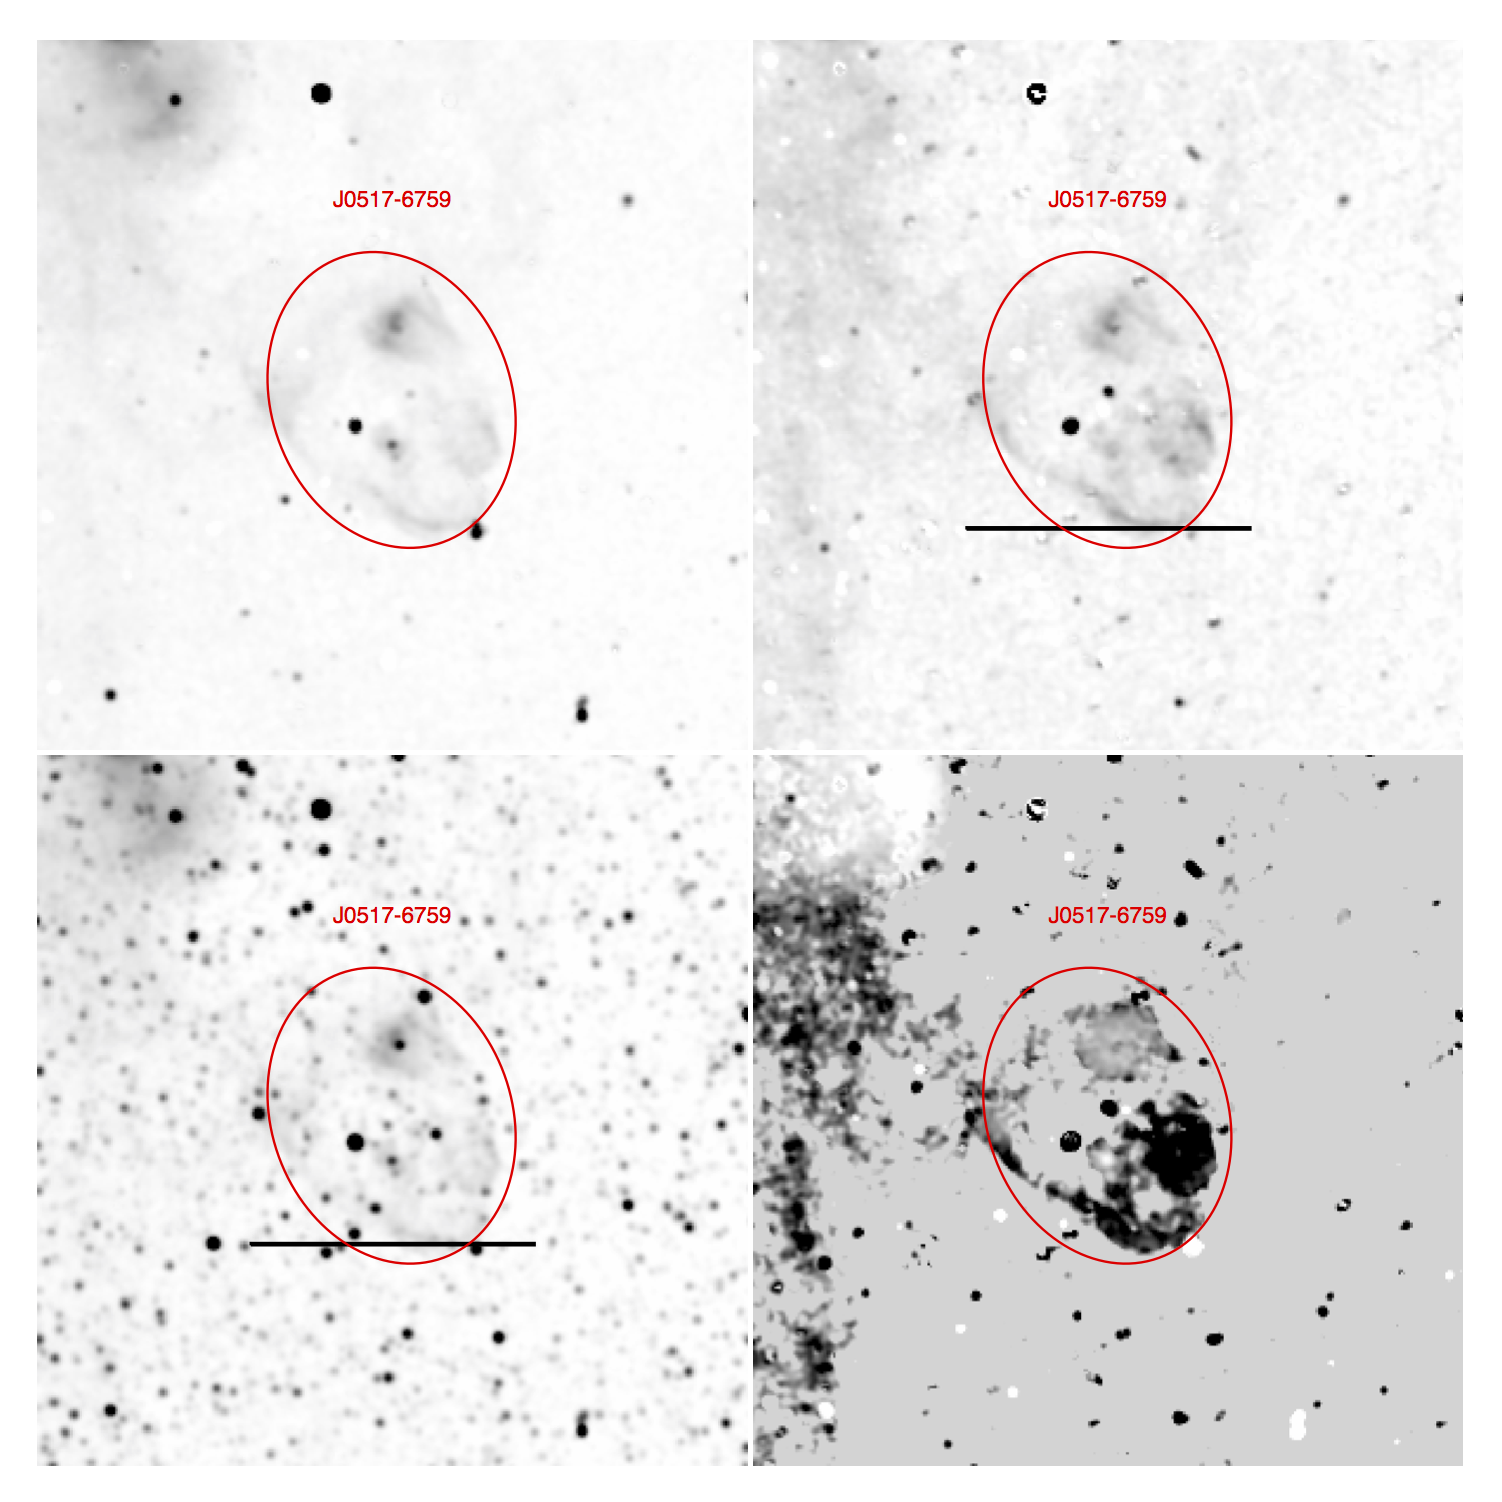
\includegraphics[width=11.cm]{snapshots/J0517-6759.png}
\end{figure}

\newpage
{\bf J0518-6939 = B0519-69.7 = N120  (field shown is 5 arcmin)}  
 
SNR shell center:   5:18:43.1  -69:39:11.0   

N-S slit; center on westernmost star of triple near east rim; offset W 3$^{\prime\prime}$

Scan:  West  75 $^{\prime\prime}$

Scan rate:  $-225 ^{\prime\prime}$/hr for 20 min exposures

Date/Frames:  Nite 3, frames 211-213

Exposure Times:  3 x 1200 s

May be hard; lots of background
\begin{figure}
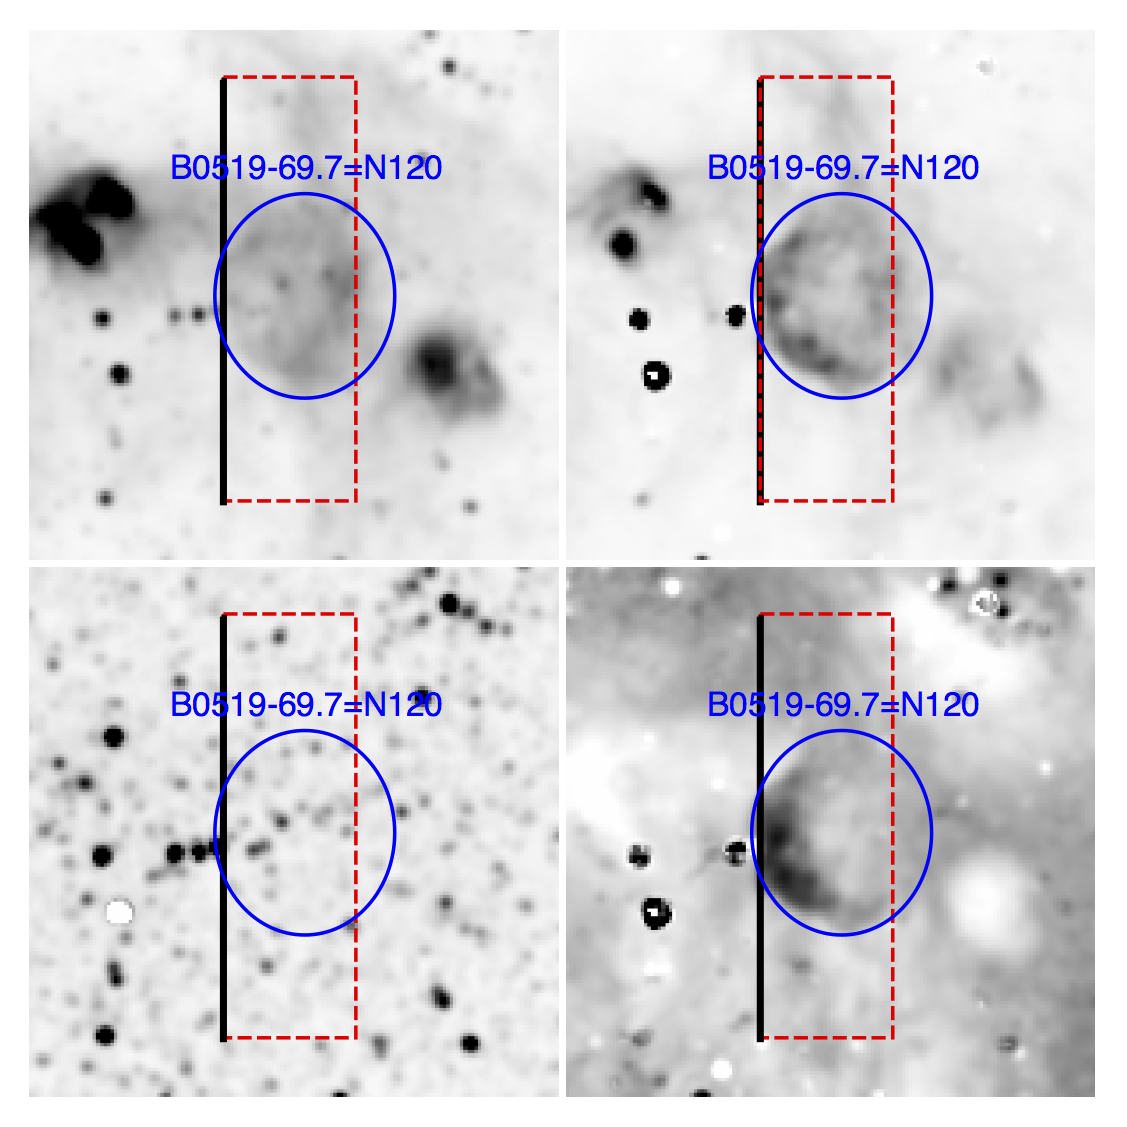
\includegraphics[width=12.5cm]{snapshots/N120_5arcmin.png}
\end{figure}

\newpage
{\bf J0518-6939 = B0519-69.7 = N120  (Longslit)}  
 
Setup star (on E rim of shell):   5:18:51.0  -69:39:13     

Slit P.A. = 14$^\circ$; center on the star (red arrow)

Date/Frames:  

Exposure Times:  2 x 900 s minimum

%May be hard; lots of background
\begin{figure}
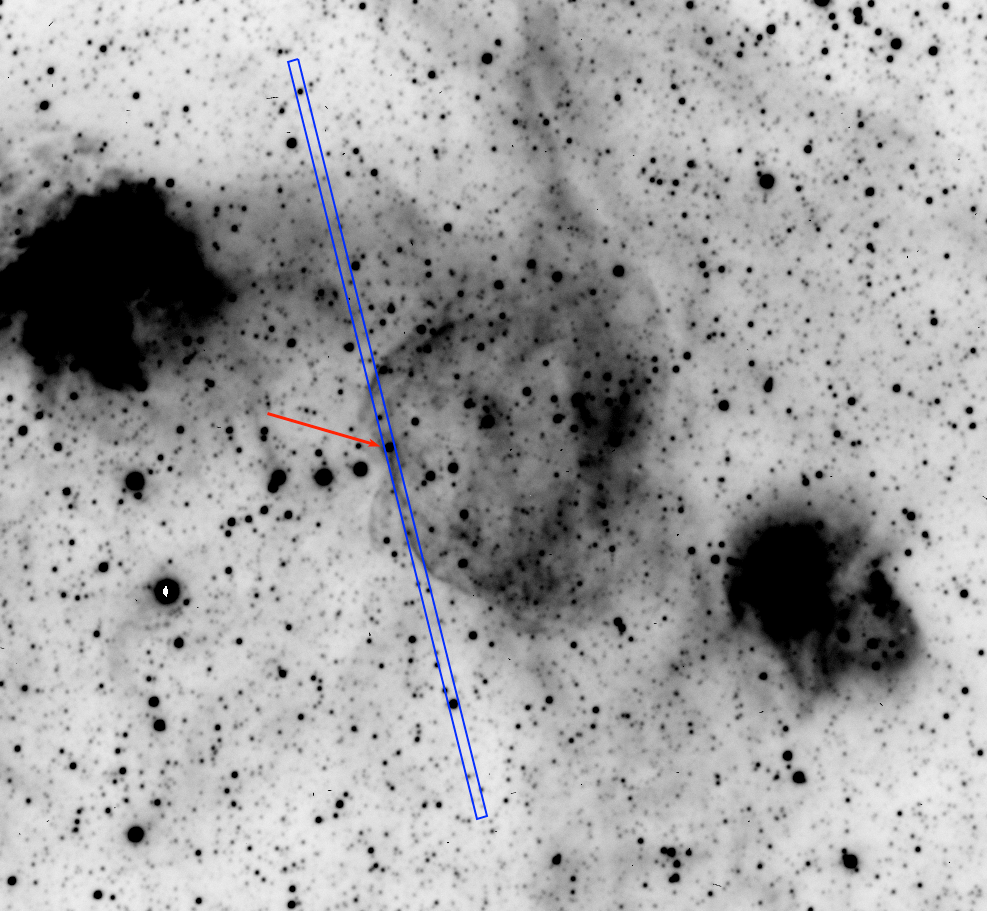
\includegraphics[width=12.5cm]{snapshots/N120_longslit.png}
\end{figure}

\newpage
{\bf J0519--6902 = B0519-69.0 (Balmer-dominated; 5 arcmin field)}  
 
Slit Center:   5:19:31.401,-69:02:16.171 N-S

Scan:  East

Scan rate:  

Date/Frames:

Exposure Times:  

\begin{figure}
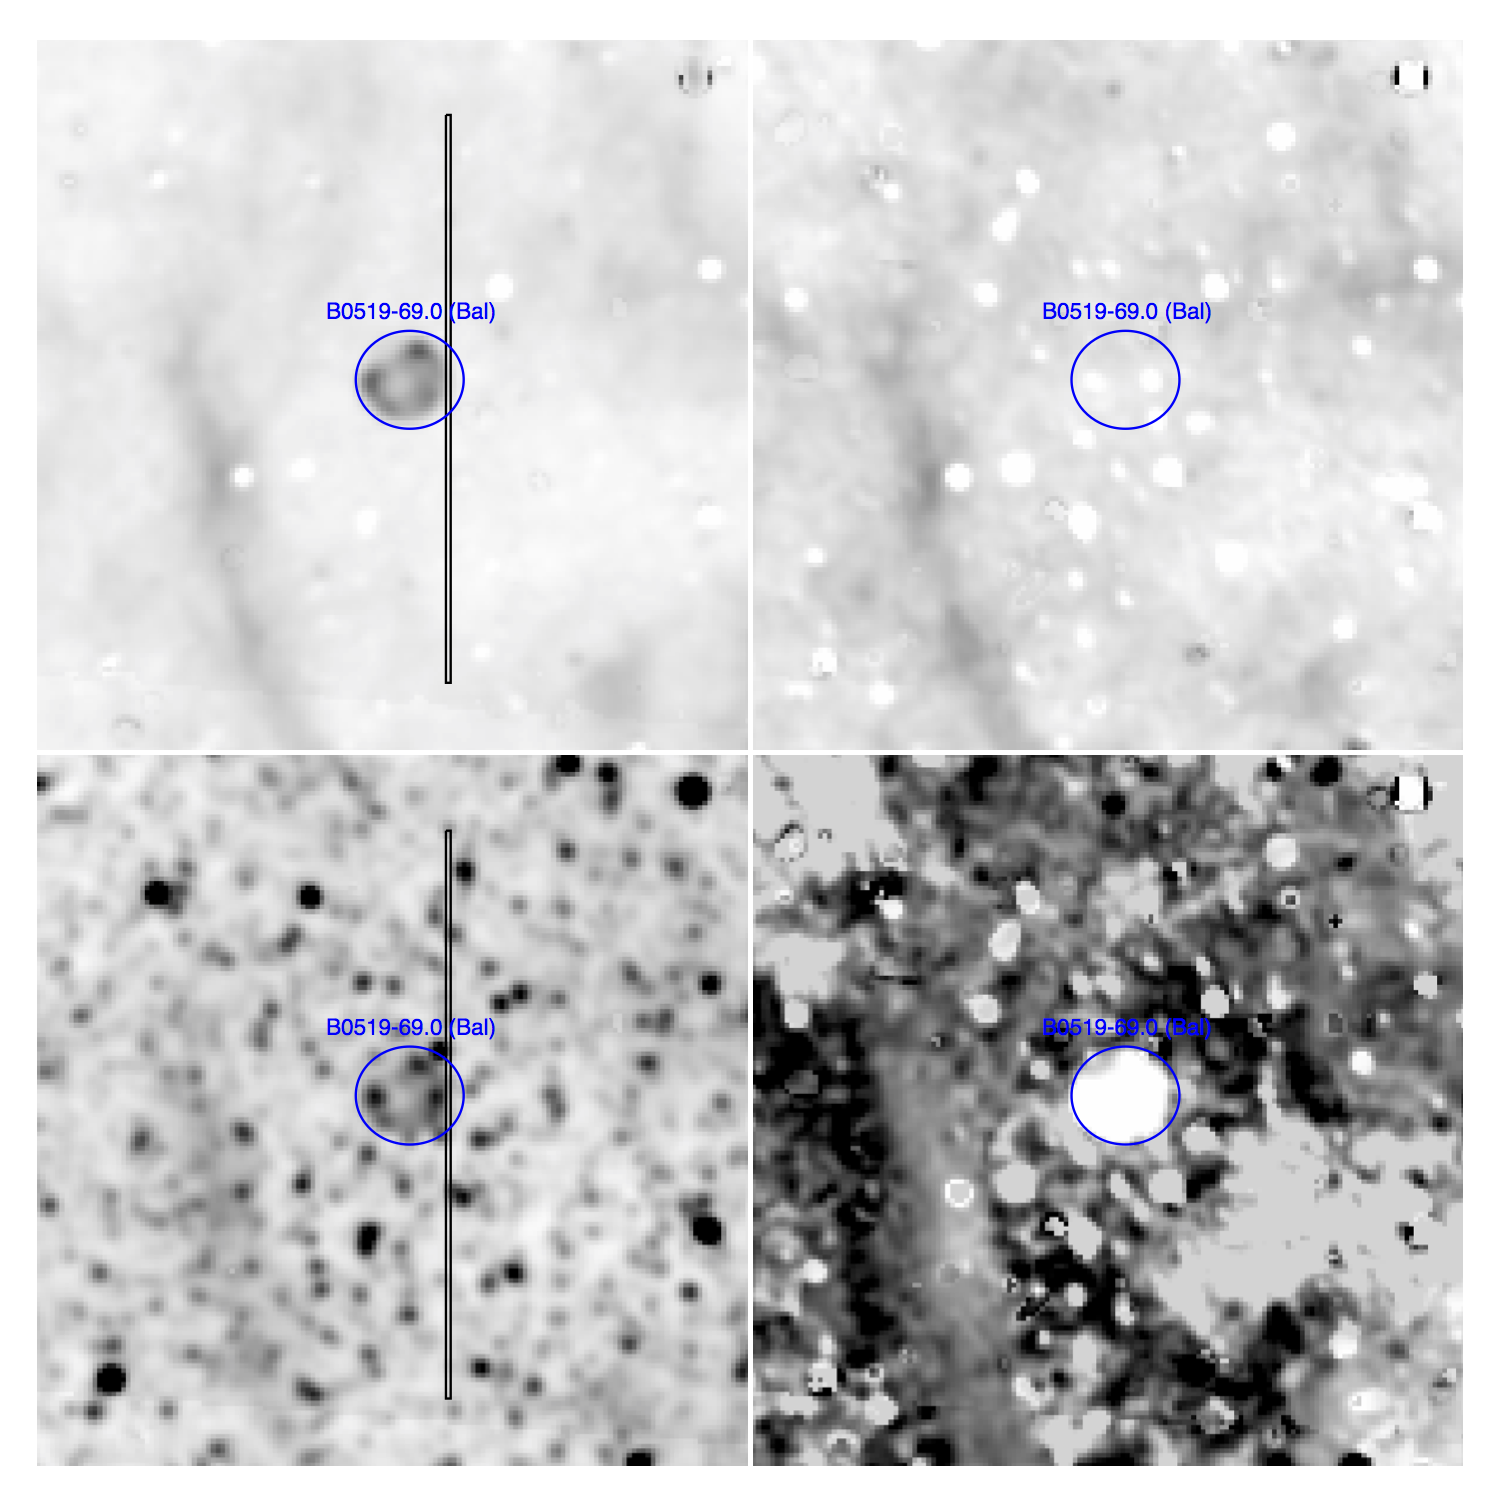
\includegraphics[width=11.cm]{snapshots/B0519-690_5arcmin.png}
\end{figure}

\newpage
{\bf J0519--6925 = B0520-69.4 (5 arcmin field)}  \ \ Surf Brightness 0.5 E-15 ergs/cm$^2/$s/arcsec$^2$
 
SNR Center:   5:19:45.1  -69:25:58.0, \ \  E-W slit 

Center on marked star S of shell; offset W 39\arcsec, N 25\arcsec

Scan:  North 140\arcsec

Scan rate:  + 280\arcsec/hr \ \ in Decl.  for 1800 s exposure

Date/Frames/Exposures:

\vspace{0.20in}
{\bf Longslit:}  from starting position, offset N 90\arcsec\ = 115\arcsec\ from ref star

{\bf Alternative longslit:}  from starting position, offset N 6\arcsec\ = 31\arcsec\ from ref star


(revised based on Goodman images --- next page)

\begin{figure}
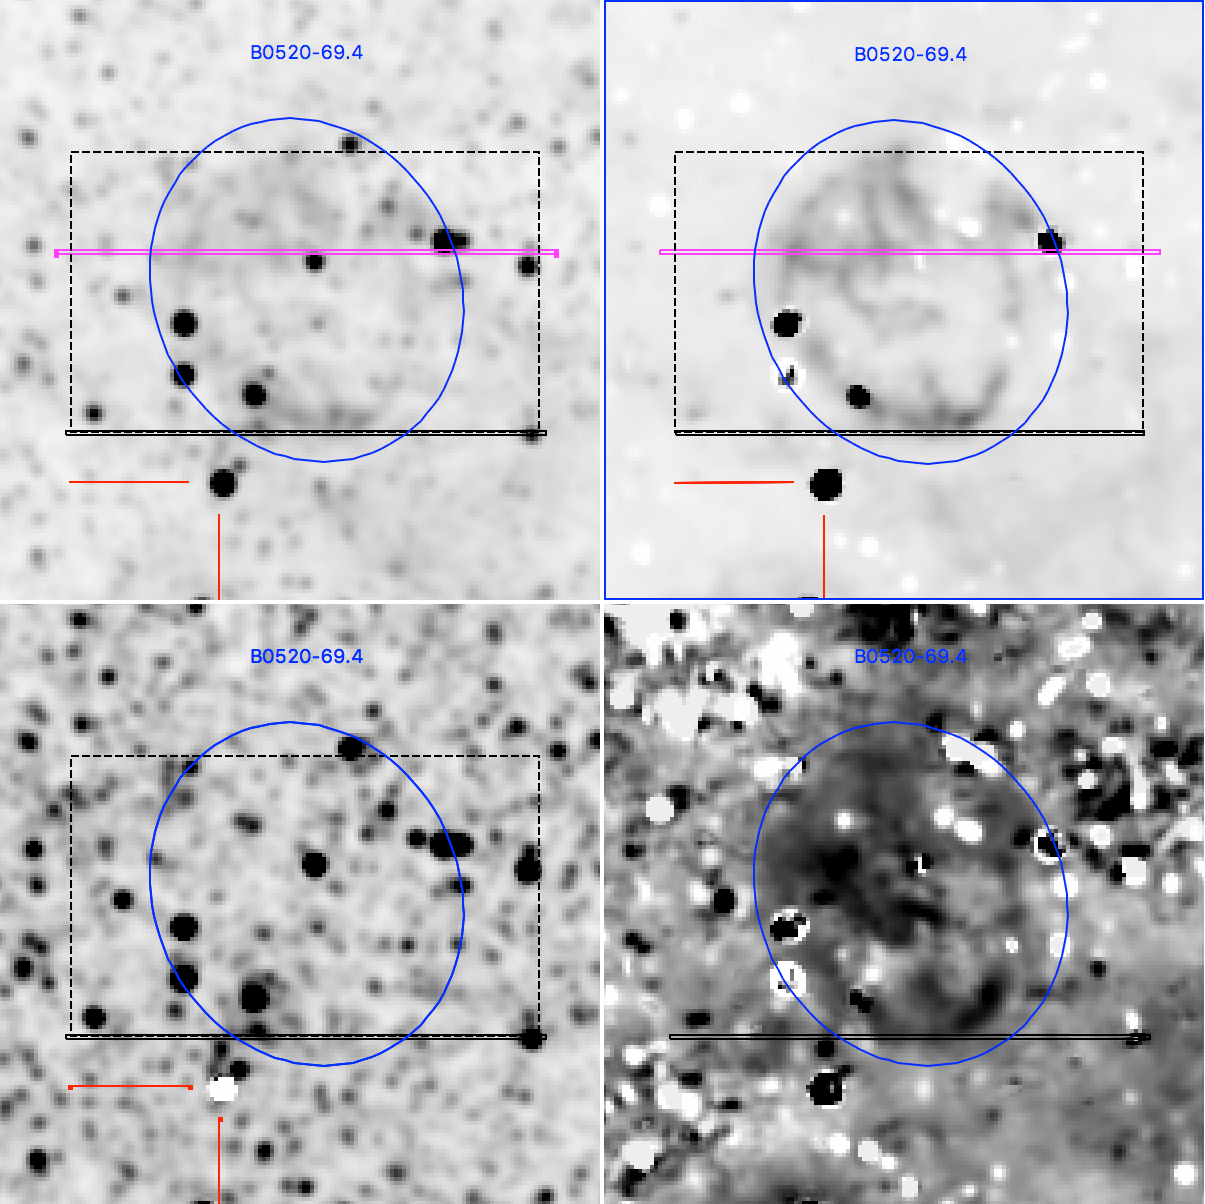
\includegraphics[width=12.5cm]{snapshots/B0520_694_5arcmin.png}
\end{figure}

\newpage
{\bf J0519--6925 = B0520-69.4 Longslit}
 
 P.A. = 100$^\circ$
 
From marked star (same one as for scanning)
offset W 42.3\arcsec, N 121\arcsec

Date/Frames/Exposures:


\begin{figure}
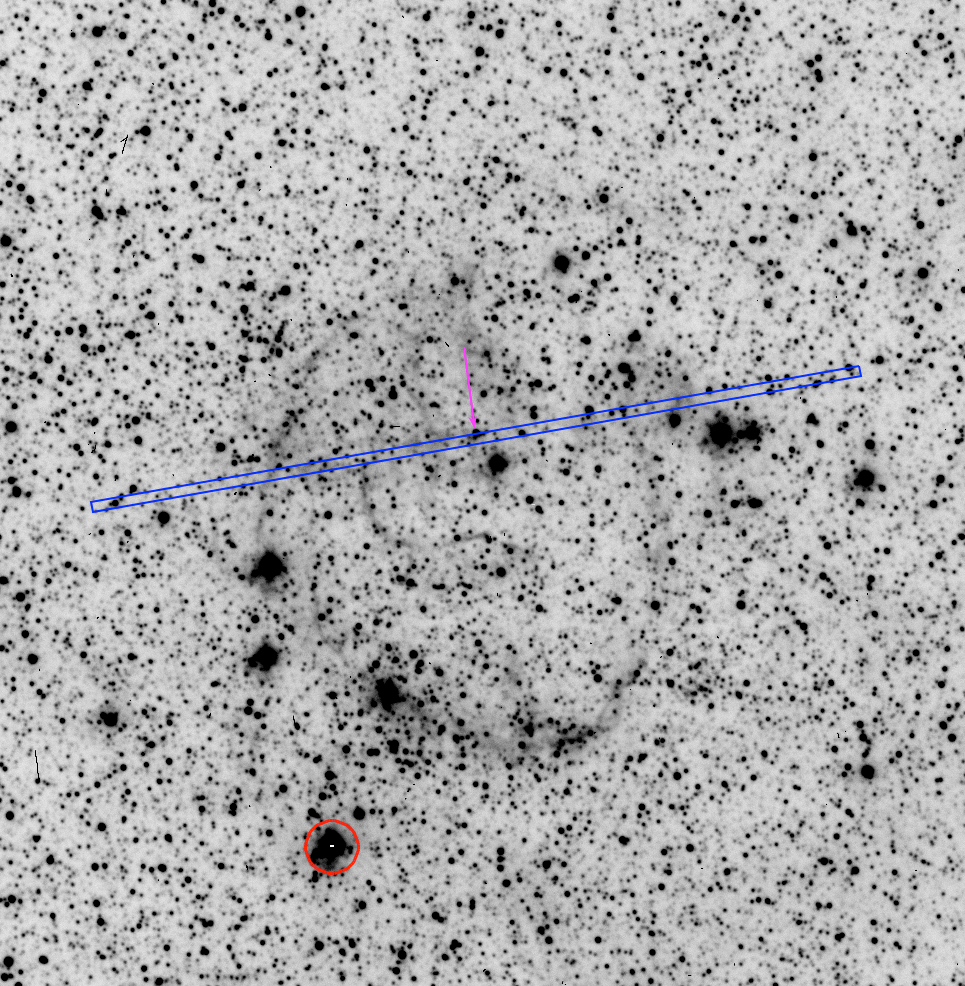
\includegraphics[width=12.5cm]{snapshots/B0520_longslit.png}
\end{figure}



\newpage
{\bf J0521-6542 = DEML142}  
 
Slit Center:   5:21:26.390   -65:43:10.137   N-S

Scan:  East

Scan rate:  

Date/Frames:

Exposure Times:  

\begin{figure}
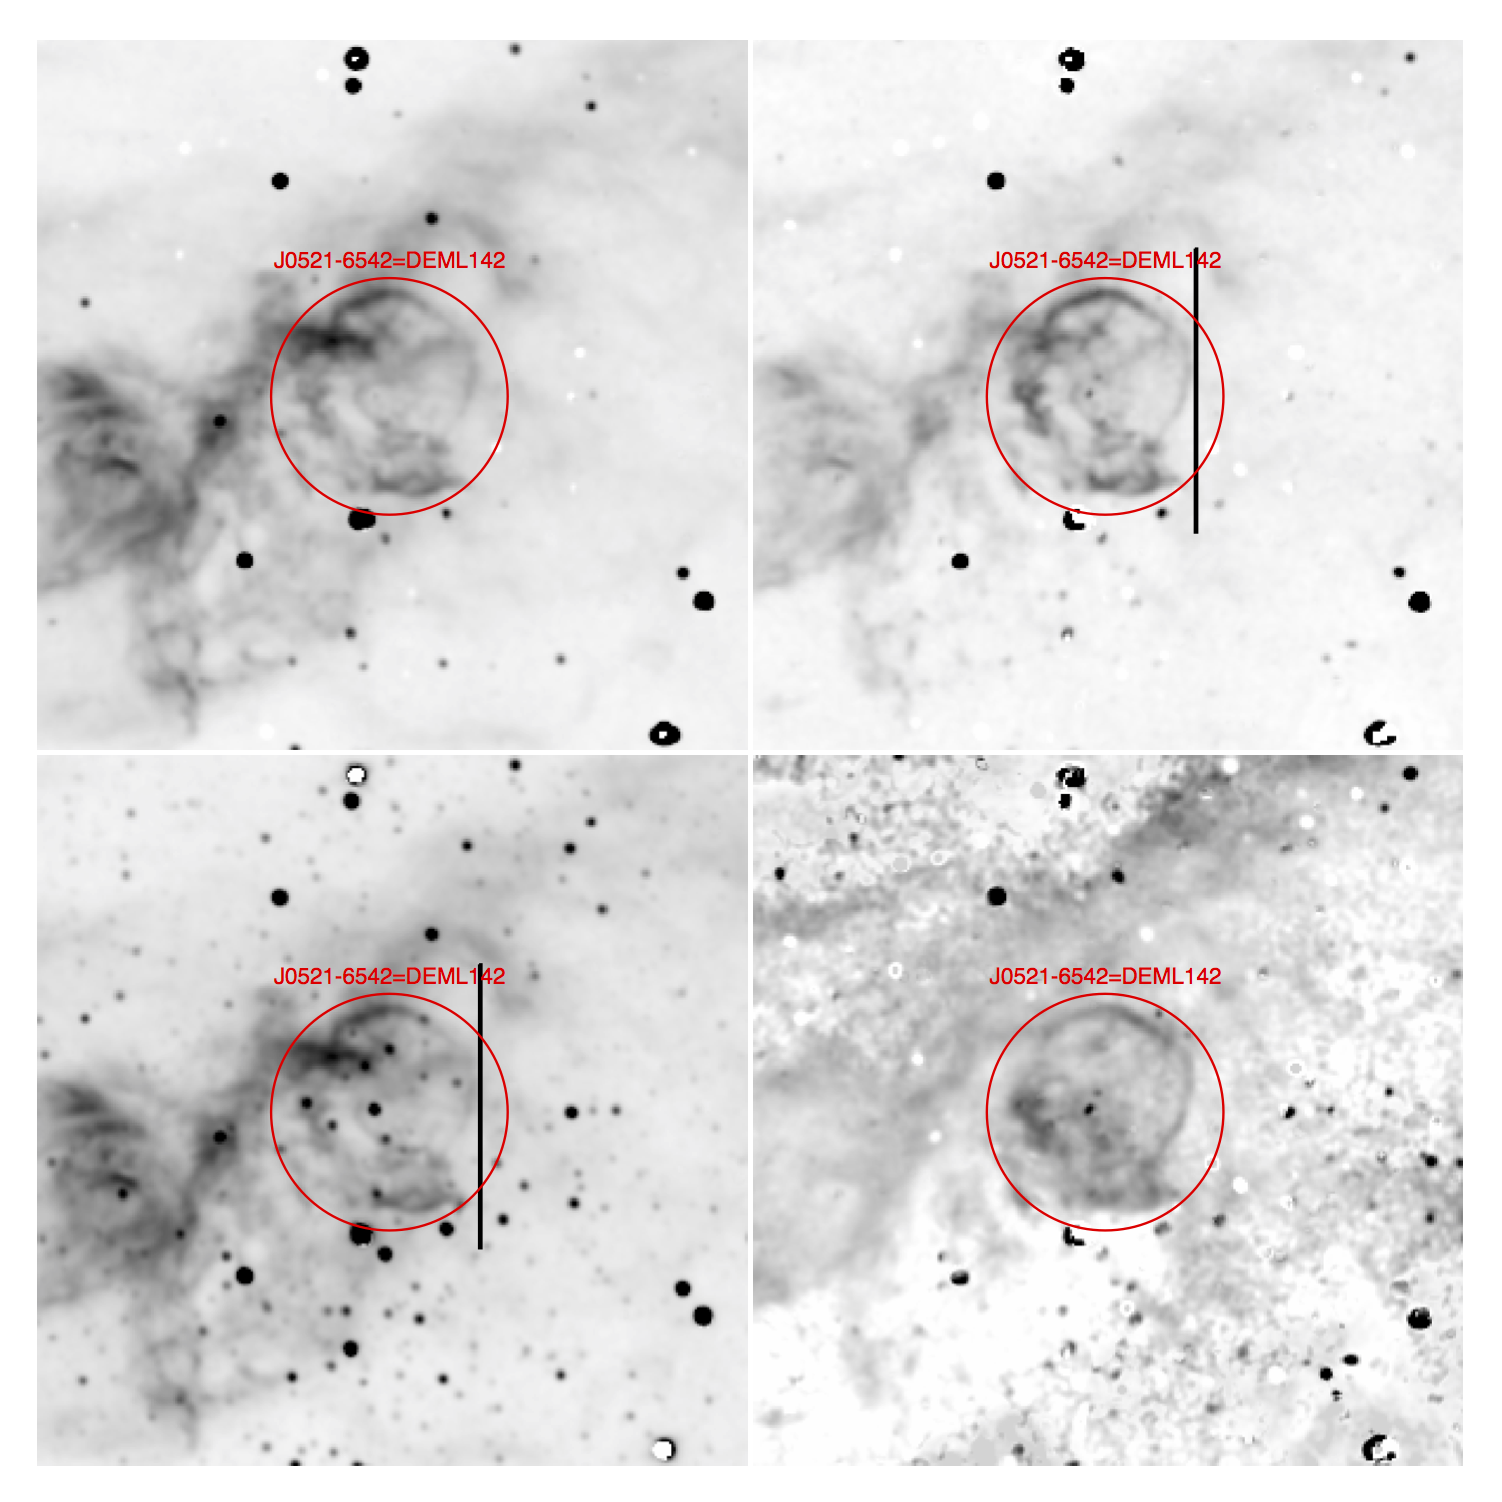
\includegraphics[width=11.cm]{snapshots/J0521-6542.png}
\end{figure}

\newpage
{\bf J0523-6753 = N441}  
 
Slit Center:   5:22:42.636  -67:53:09.888 N-S

Scan:  East

Scan rate:  

Date/Frames:

Exposure Times:  

\begin{figure}
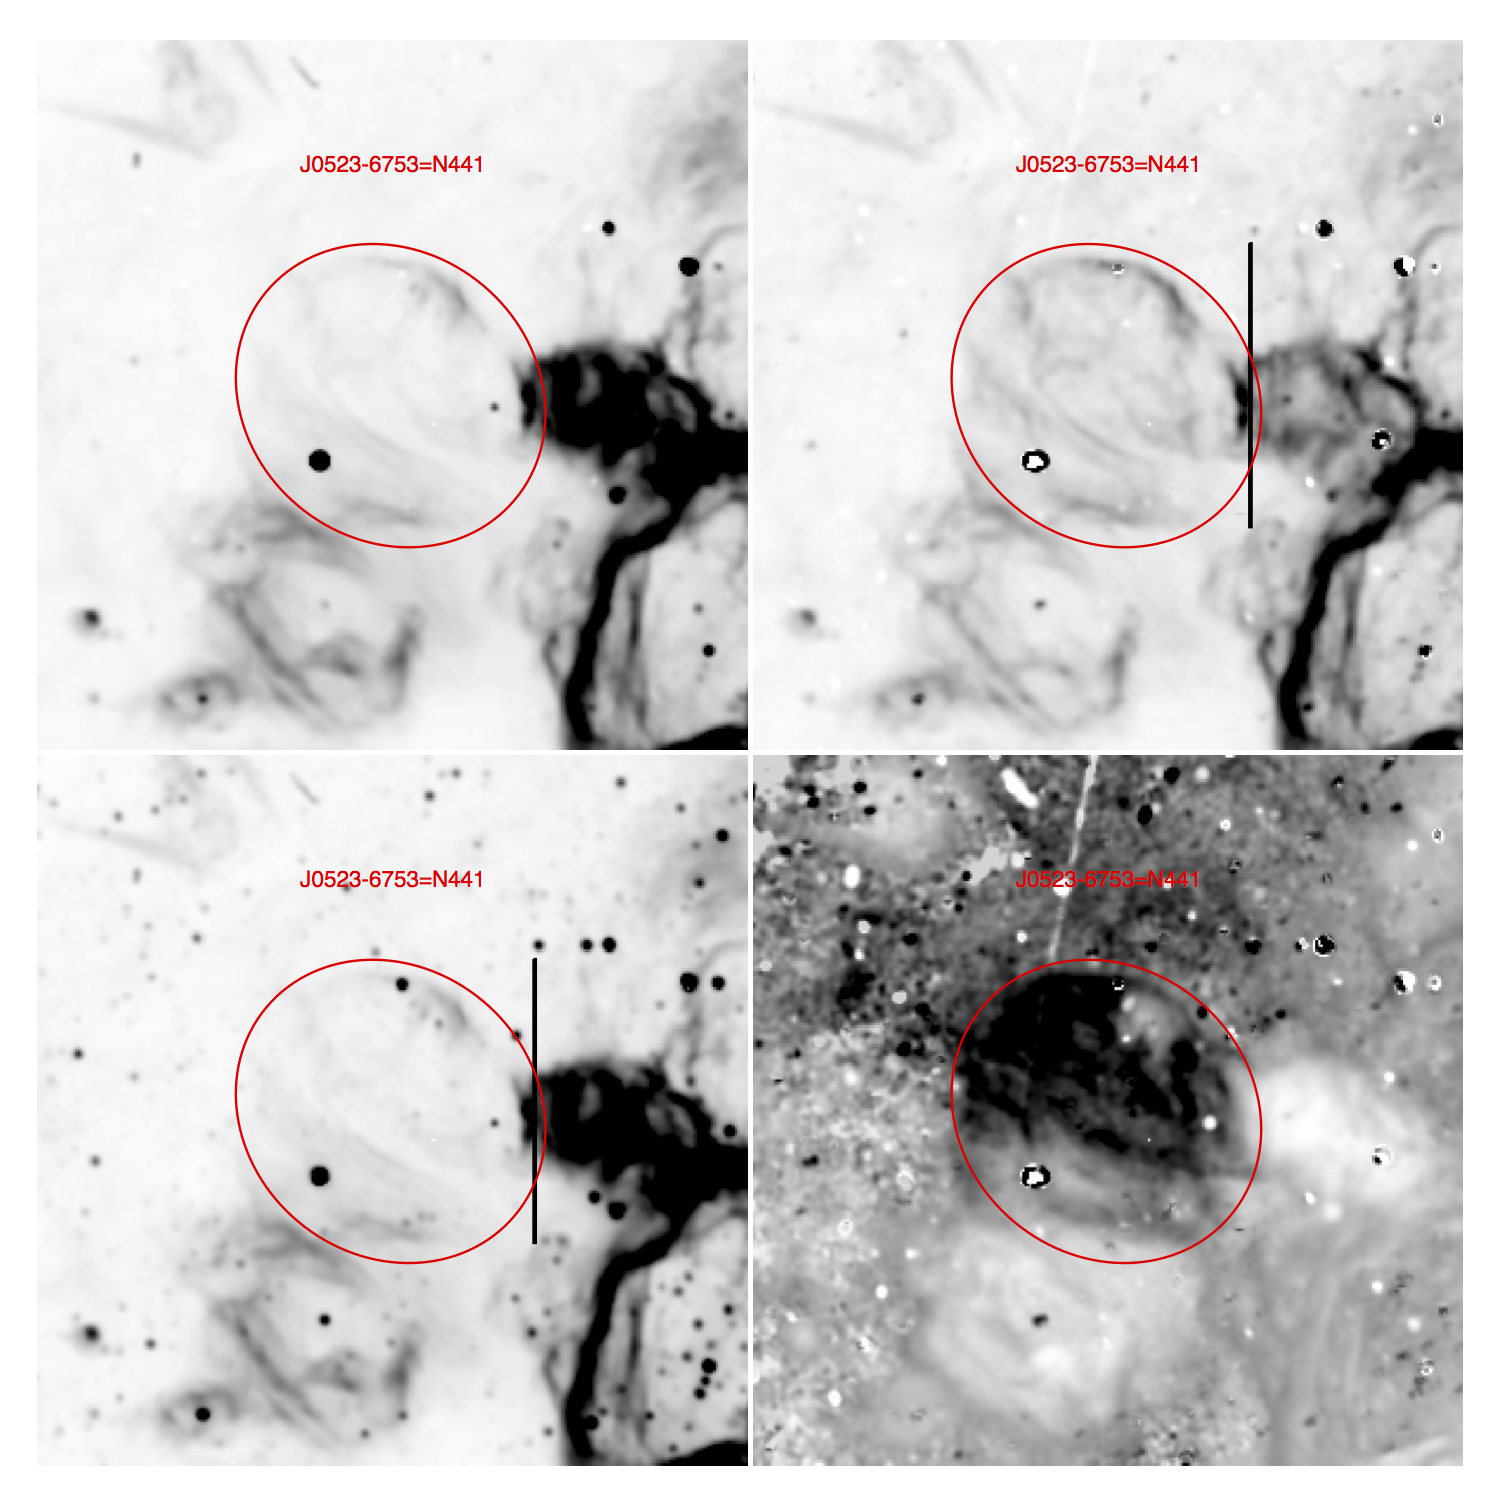
\includegraphics[width=11.cm]{snapshots/J0523-6753.png}
\end{figure}

\newpage
{\bf J0524-6623 = B0524-66.4}  
 
Slit Center:   5:24:05.457   -66:23:39.150 N-S

Scan:  East

Scan rate:  

Date/Frames:

Exposure Times:  

\begin{figure}
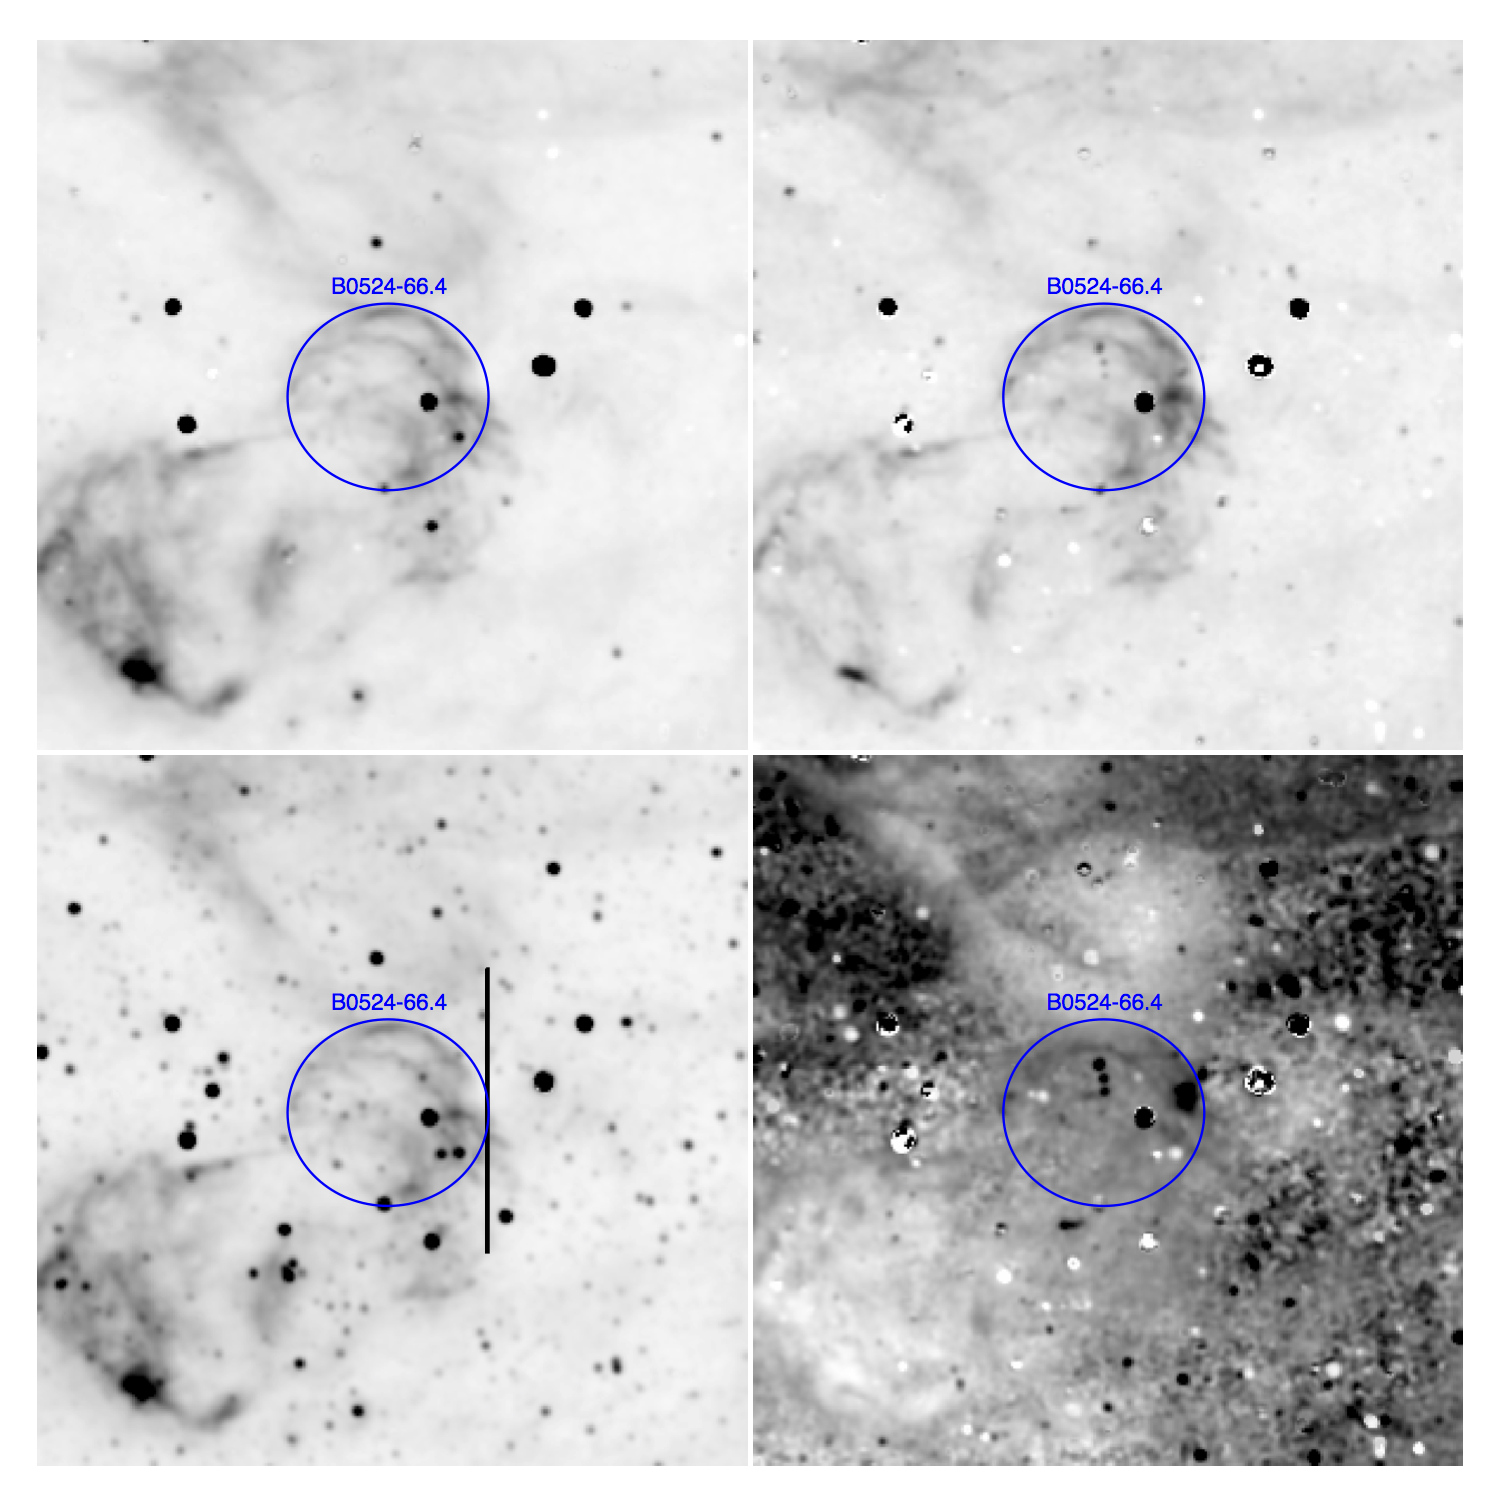
\includegraphics[width=11.cm]{snapshots/B0524-664.png}
\end{figure}


\newpage
{\bf J0525=6938 = N132D = B0525-69.6 (5 arcmin)}  
 
SNR Center:   5:25:02.7   -69:38:29     E-W slit

Center on very bright star WNW of shell; offset E 98\arcsec,  N 13\arcsec

Scan:  South  105\arcsec

Scan rate:  Decl. -210\arcsec/hr  for 30 min exposure

Date/Frames:

Exposure Times:  

\begin{figure}
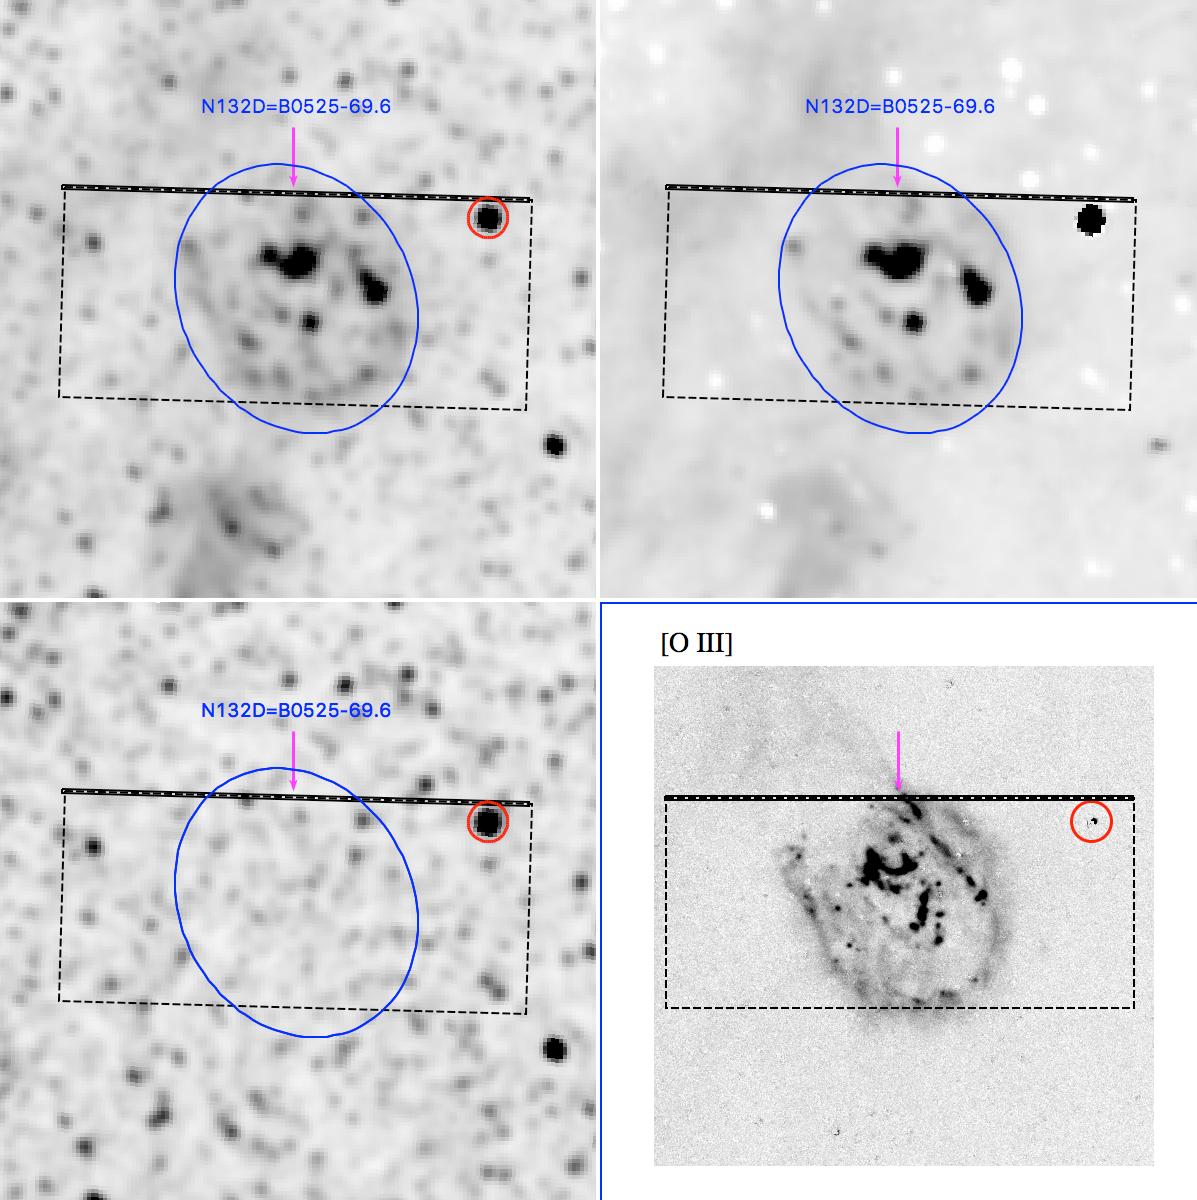
\includegraphics[width=12.5cm]{snapshots/N132D_5arcmin.png}
\end{figure}


\newpage
{\bf J0525=6559 = N49B = B0525-66.0 (5 arcmin field)}  
 
SNR Center:   5:25:29.67  -65:59:21.6;     offset 16\arcsec W;  N-S slit

Scan:  East, 32\arcsec

Scan rate:  

Date/Frames:  Nite 1, frames 277-280

Exposure Times:  2 x 10 min  +  2 x 20 min

\begin{figure}
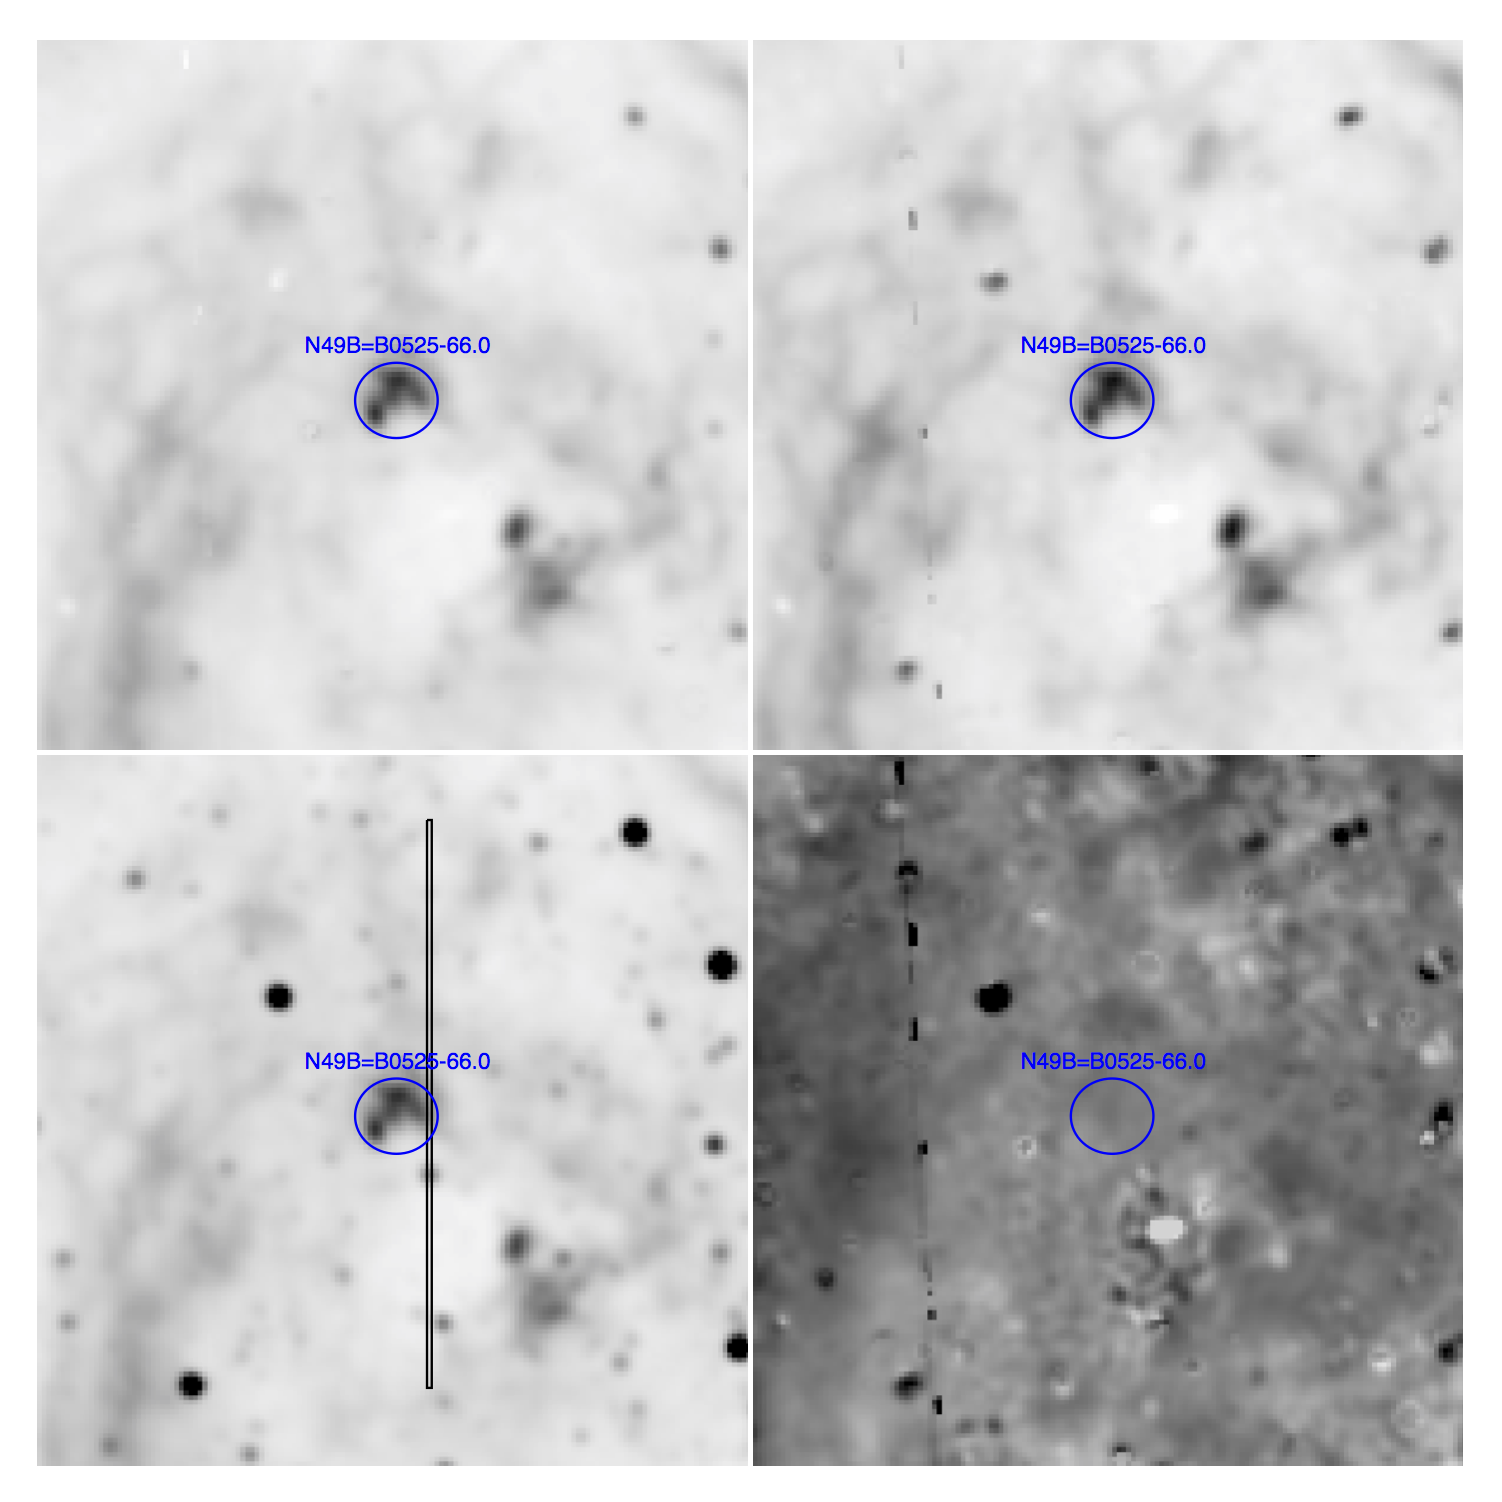
\includegraphics[width=11.cm]{snapshots/N49B_5arcmin.png}
\end{figure}

\newpage
{\bf J0525=6559 = N49B Longslit}  
 
Setup star:   5:25:27.5  -65:59:47;

Slit P.A. = $-32^\circ = 148^\circ$;     offset E 22.8\arcsec,  N 21\arcsec   

Date/Frames:  Nite 5, frames: 

Exposure Times:  2 x 900 s min

\begin{figure}
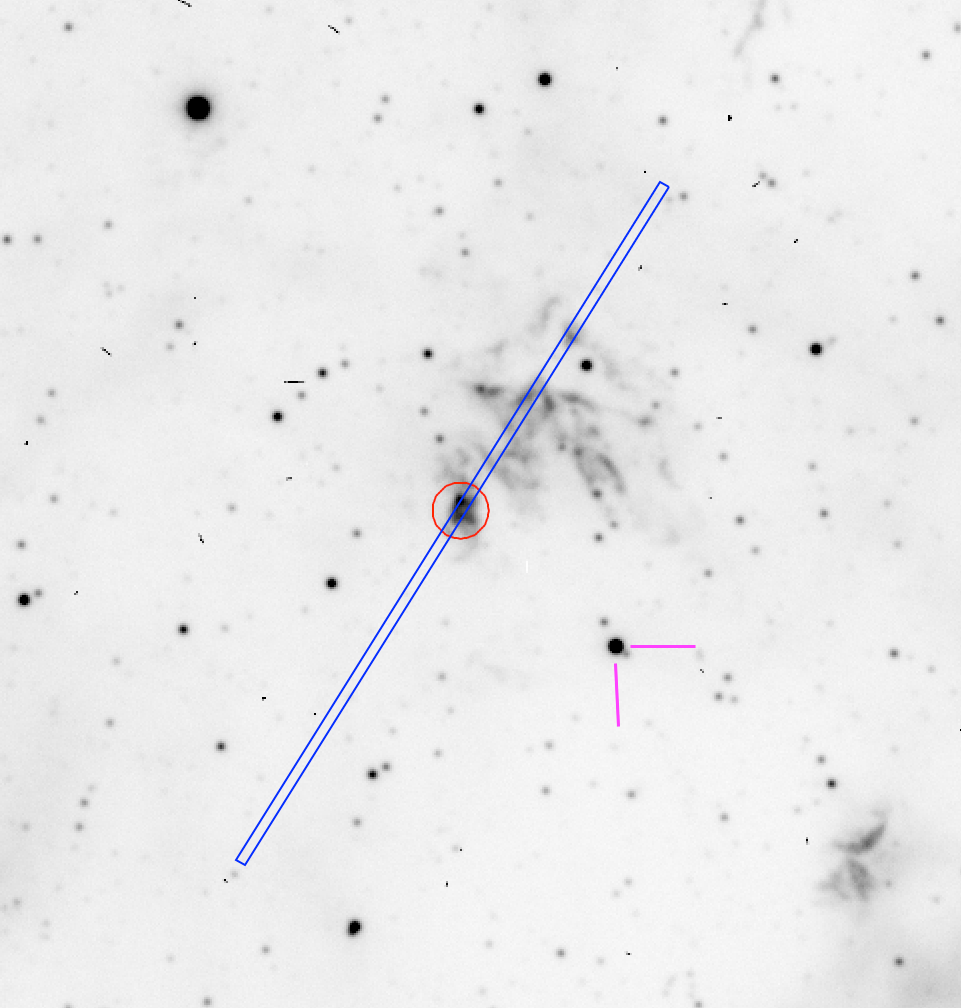
\includegraphics[width=12.5cm]{snapshots/N49B_longslit.png}
\end{figure}


\newpage
{\bf J0526-6604 = N49 = B0525-66.1 (5 arcmin field)}  
 
SNR Center:   5:26:00.1   -66:04:59.0;  offset 75\arcsec W;      N-S slit

Scan:  East   150\arcsec

Scan rate:    600\arcsec/hr

Date/Frames:  Nite 1, frames 258-264

Exposure Times:  4 x 10 min

\begin{figure}
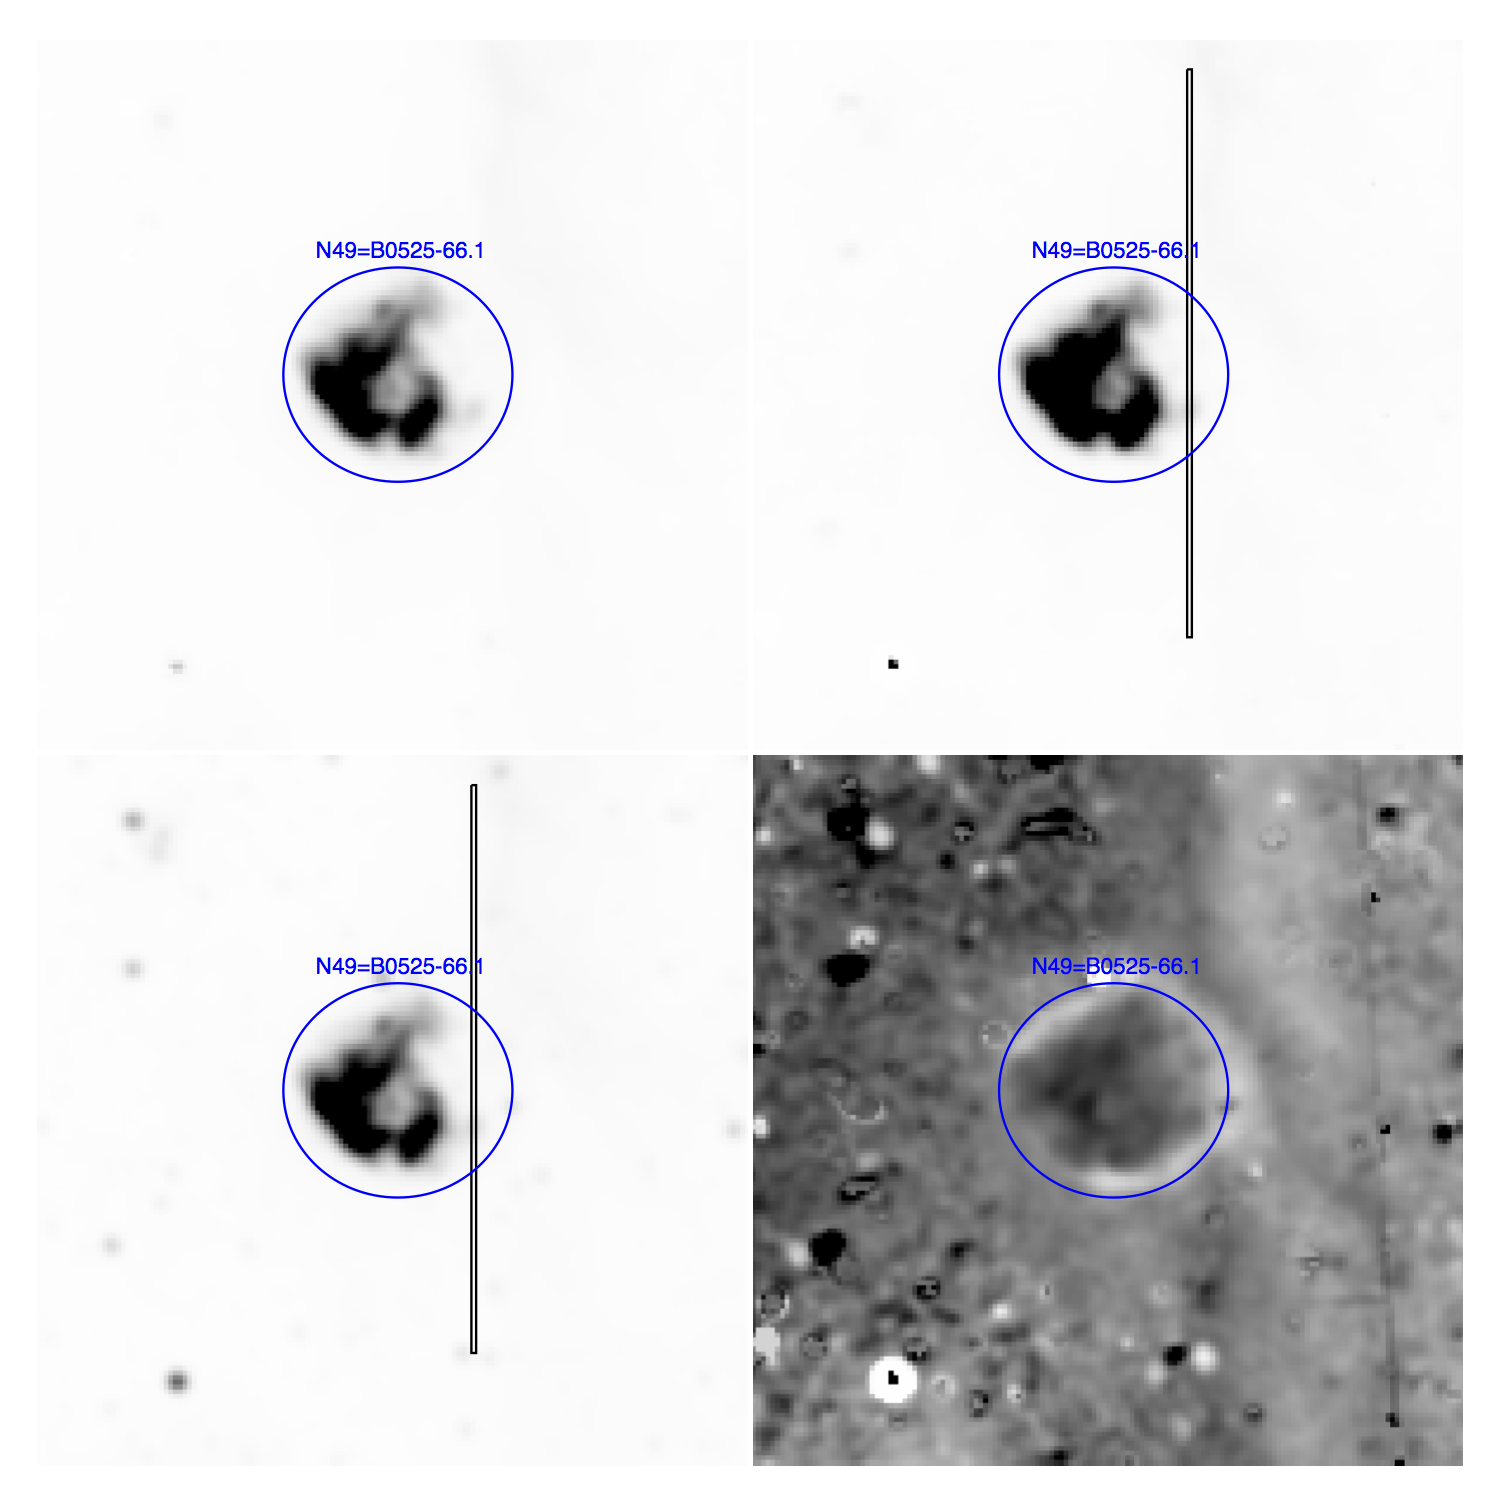
\includegraphics[width=11.cm]{snapshots/N49_5arcmin.png}
\end{figure}

\newpage
{\bf J0527-6912 = B0528-67.2}  
 
Slit Center:   5:27:24.822  -69:12:07.609 N-S

Scan:  East

Scan rate:  

Date/Frames:

Exposure Times:  

\begin{figure}
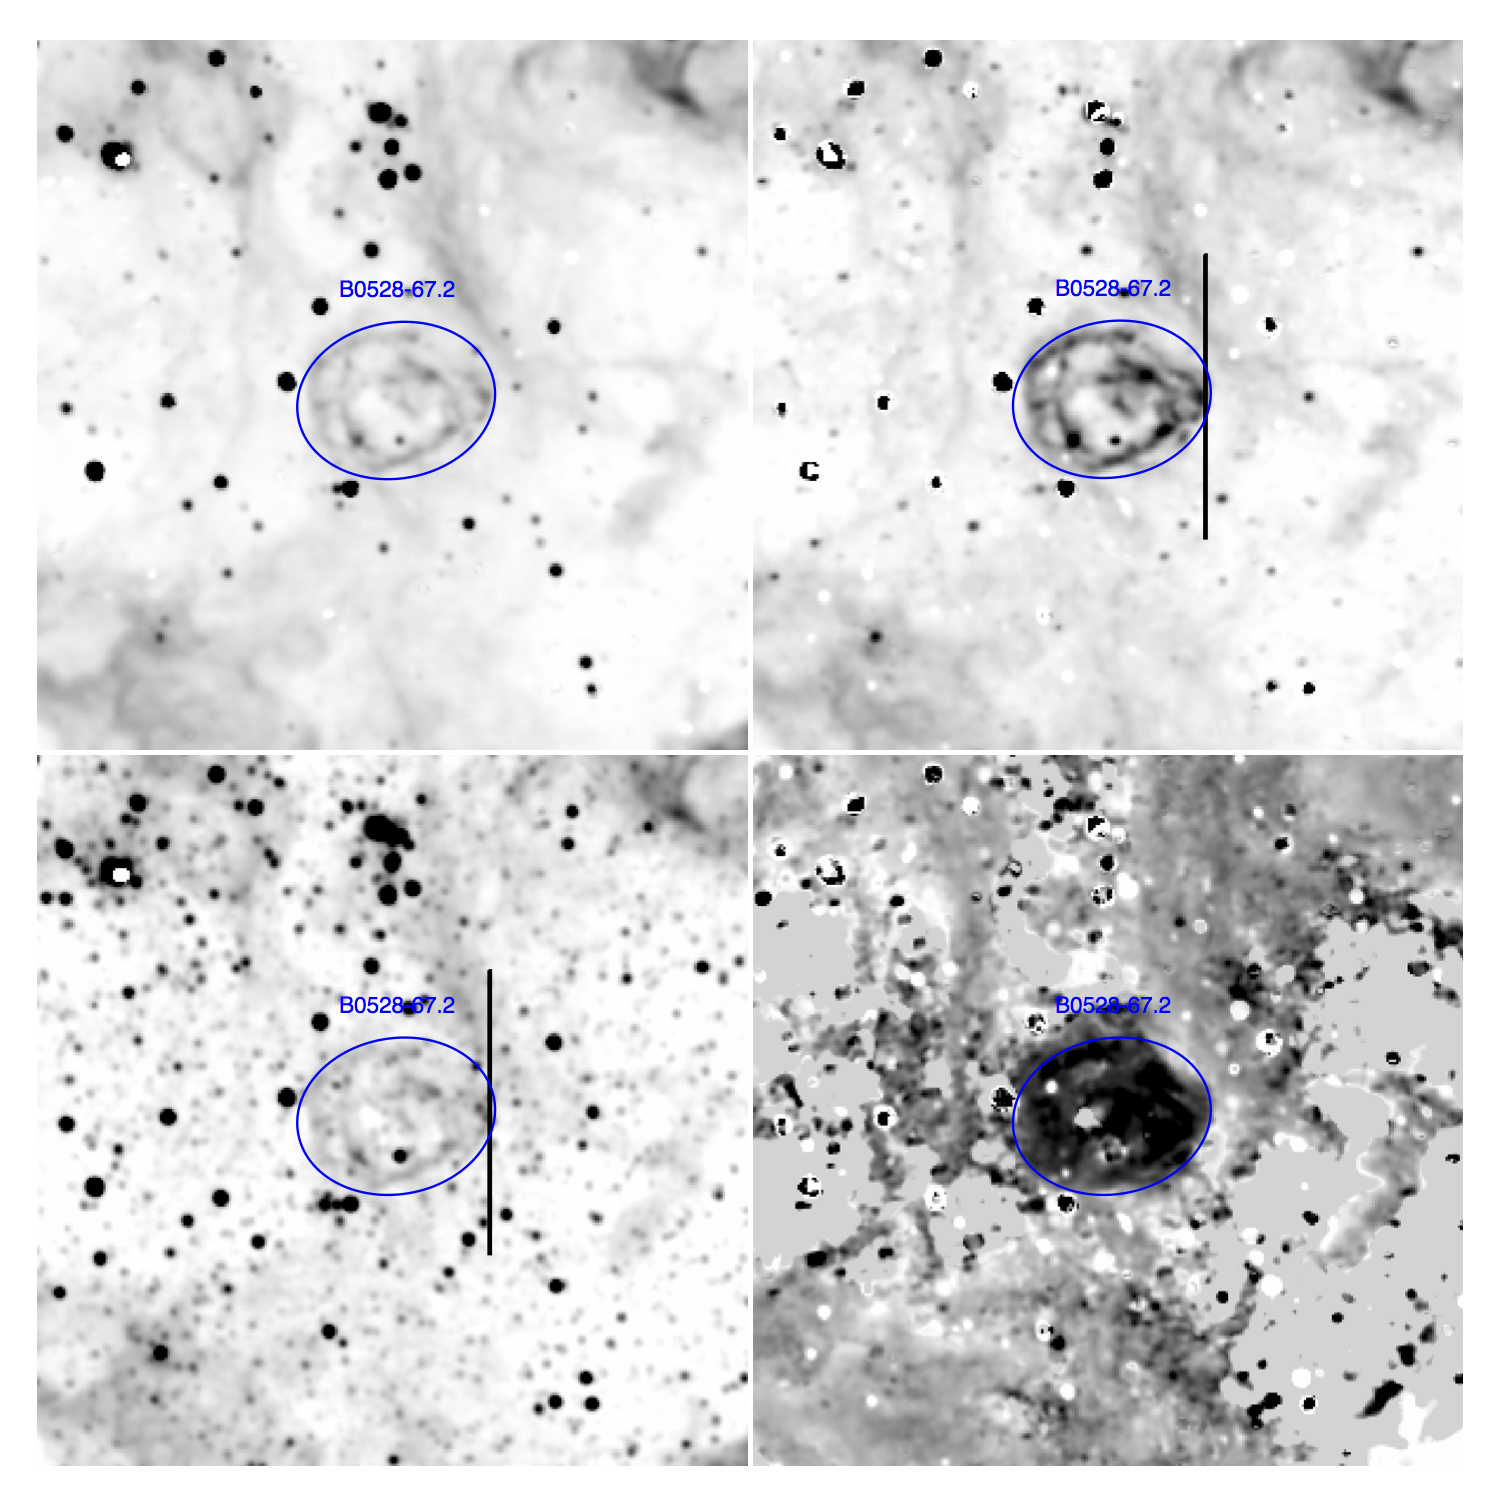
\includegraphics[width=11.cm]{snapshots/B0528-672.png}
\end{figure}

\newpage
{\bf J0527-6549 = B0527-65.8 = DEML204}  
 
Slit Center:   none; this one is TOO BIG

Scan:  East

Scan rate:  

Date/Frames:

Exposure Times:  

No snapshot yet
\begin{figure}
%\includegraphics[width=11.cm]{snapshots/xxx.png}
\end{figure}

\newpage
{\bf J0528-7104}  
 
Slit Center:   5:28:04.784,-71:07:11.216  E-W

Scan:  North

Scan rate:  

Date/Frames:

Exposure Times:  

\begin{figure}
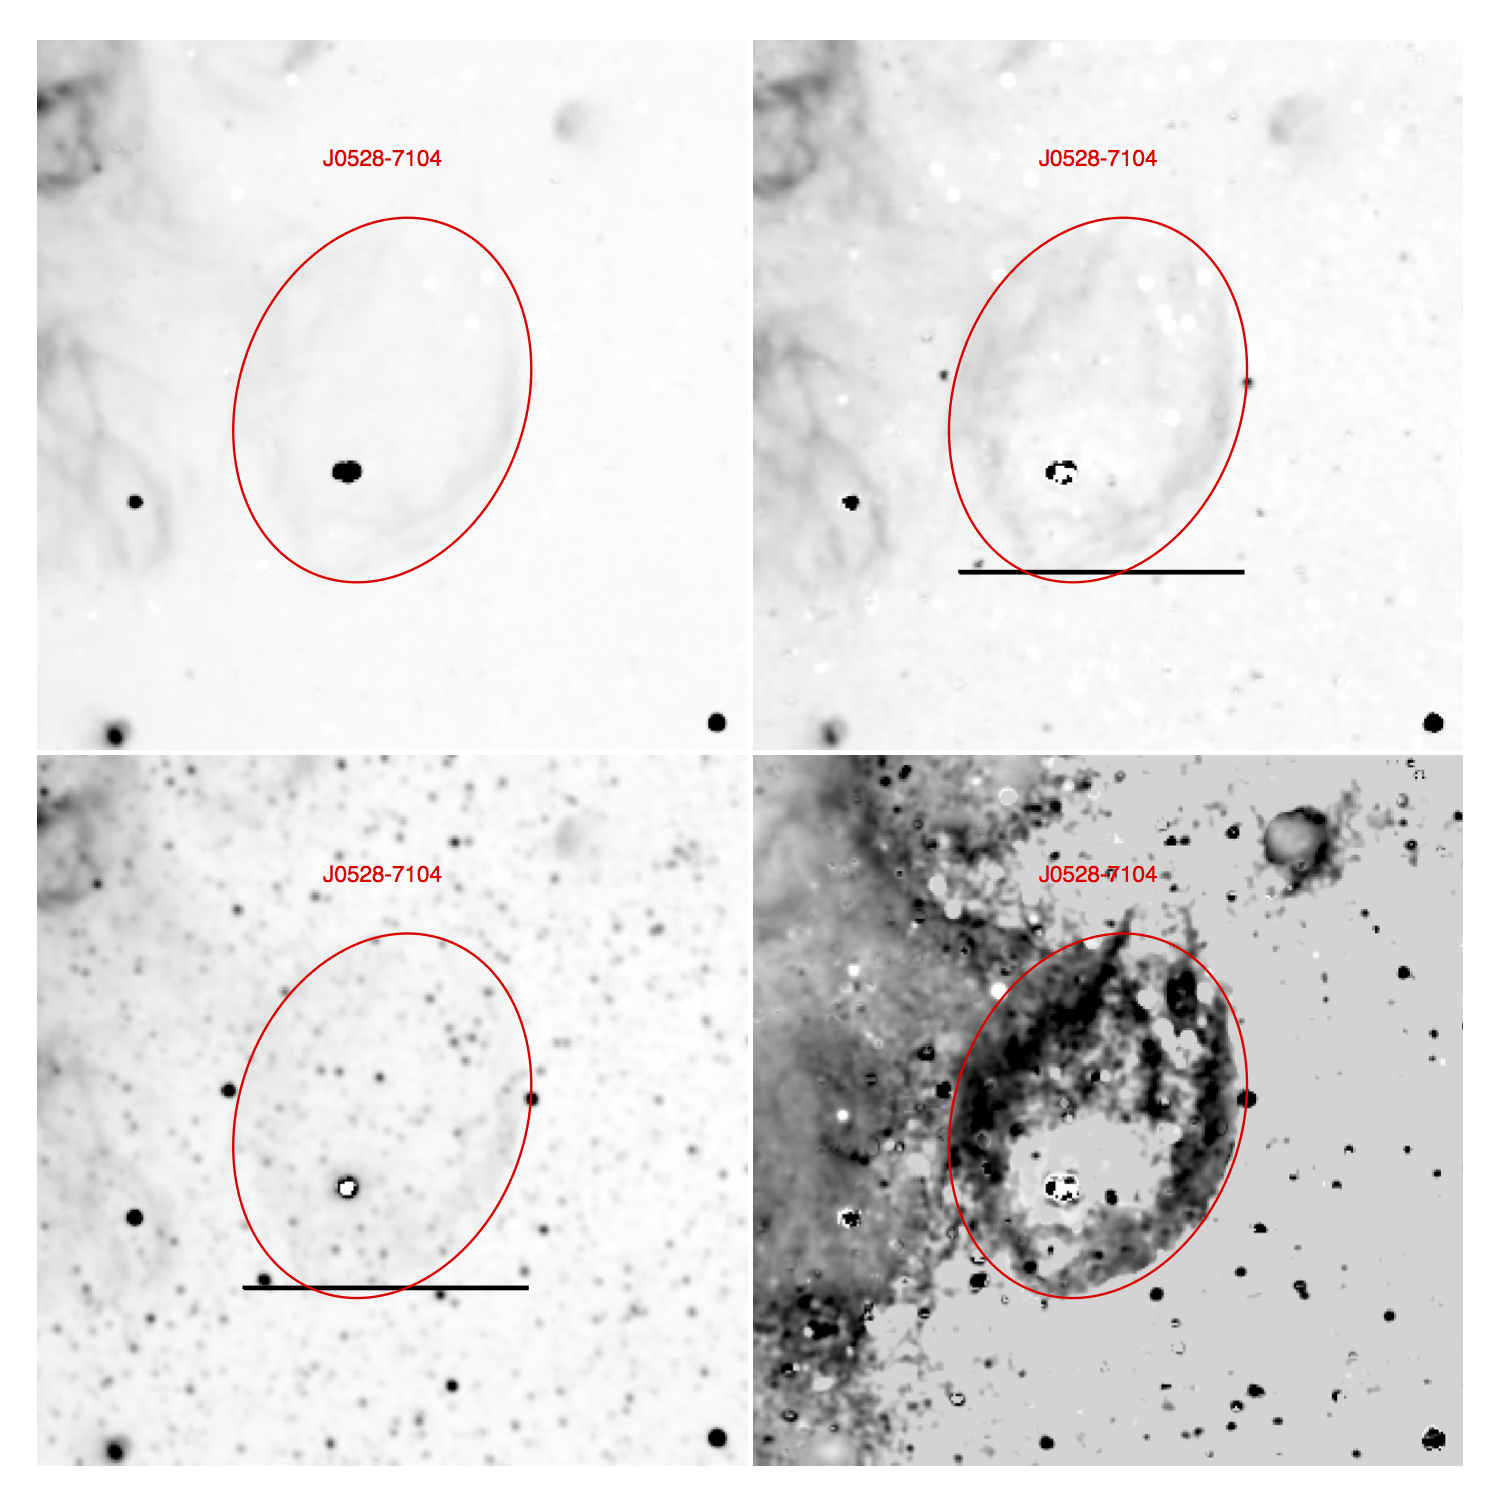
\includegraphics[width=11.cm]{snapshots/J0528-7104_big.png}
\end{figure}

\newpage
{\bf J0528-6726 = DEML205}  
 
Slit Center:   5:28:13.0  -67:29:01.9  

E-W slit; center on bright star SE of rim; offset W 83$^{\prime\prime}$, N 11$^{\prime\prime}$

Scan:  North 250$^{\prime\prime}$

Scan rate:  500 $^{\prime\prime}$/hr for 30 min

%{\bf PFW suggests that if no high-velocity emission in first frame, we move on.}

Date/Frames:   Did 3 frames, 223-225 on Nite 3

Exposure Times:   3 x 30 min

\begin{figure}
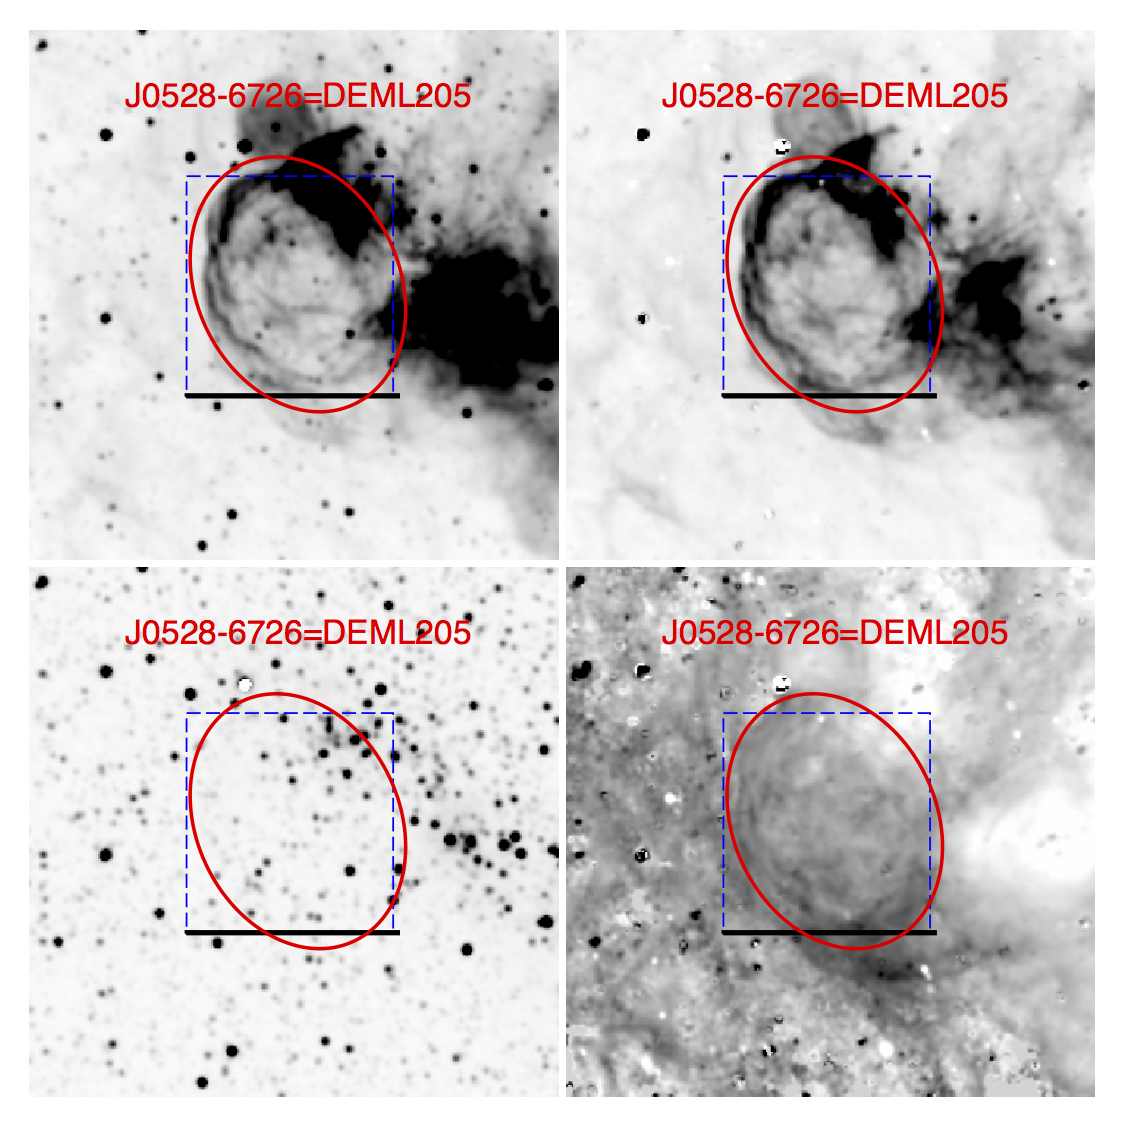
\includegraphics[width=12.5cm]{snapshots/DEML205.png}
\end{figure}

\newpage
{\bf J0530-7007 = DEML218}  
 
Slit Center:   5:30:16.284   -70:07:11.822 N-S

Scan:  East

Scan rate:  

Date/Frames:

Exposure Times:  

\begin{figure}
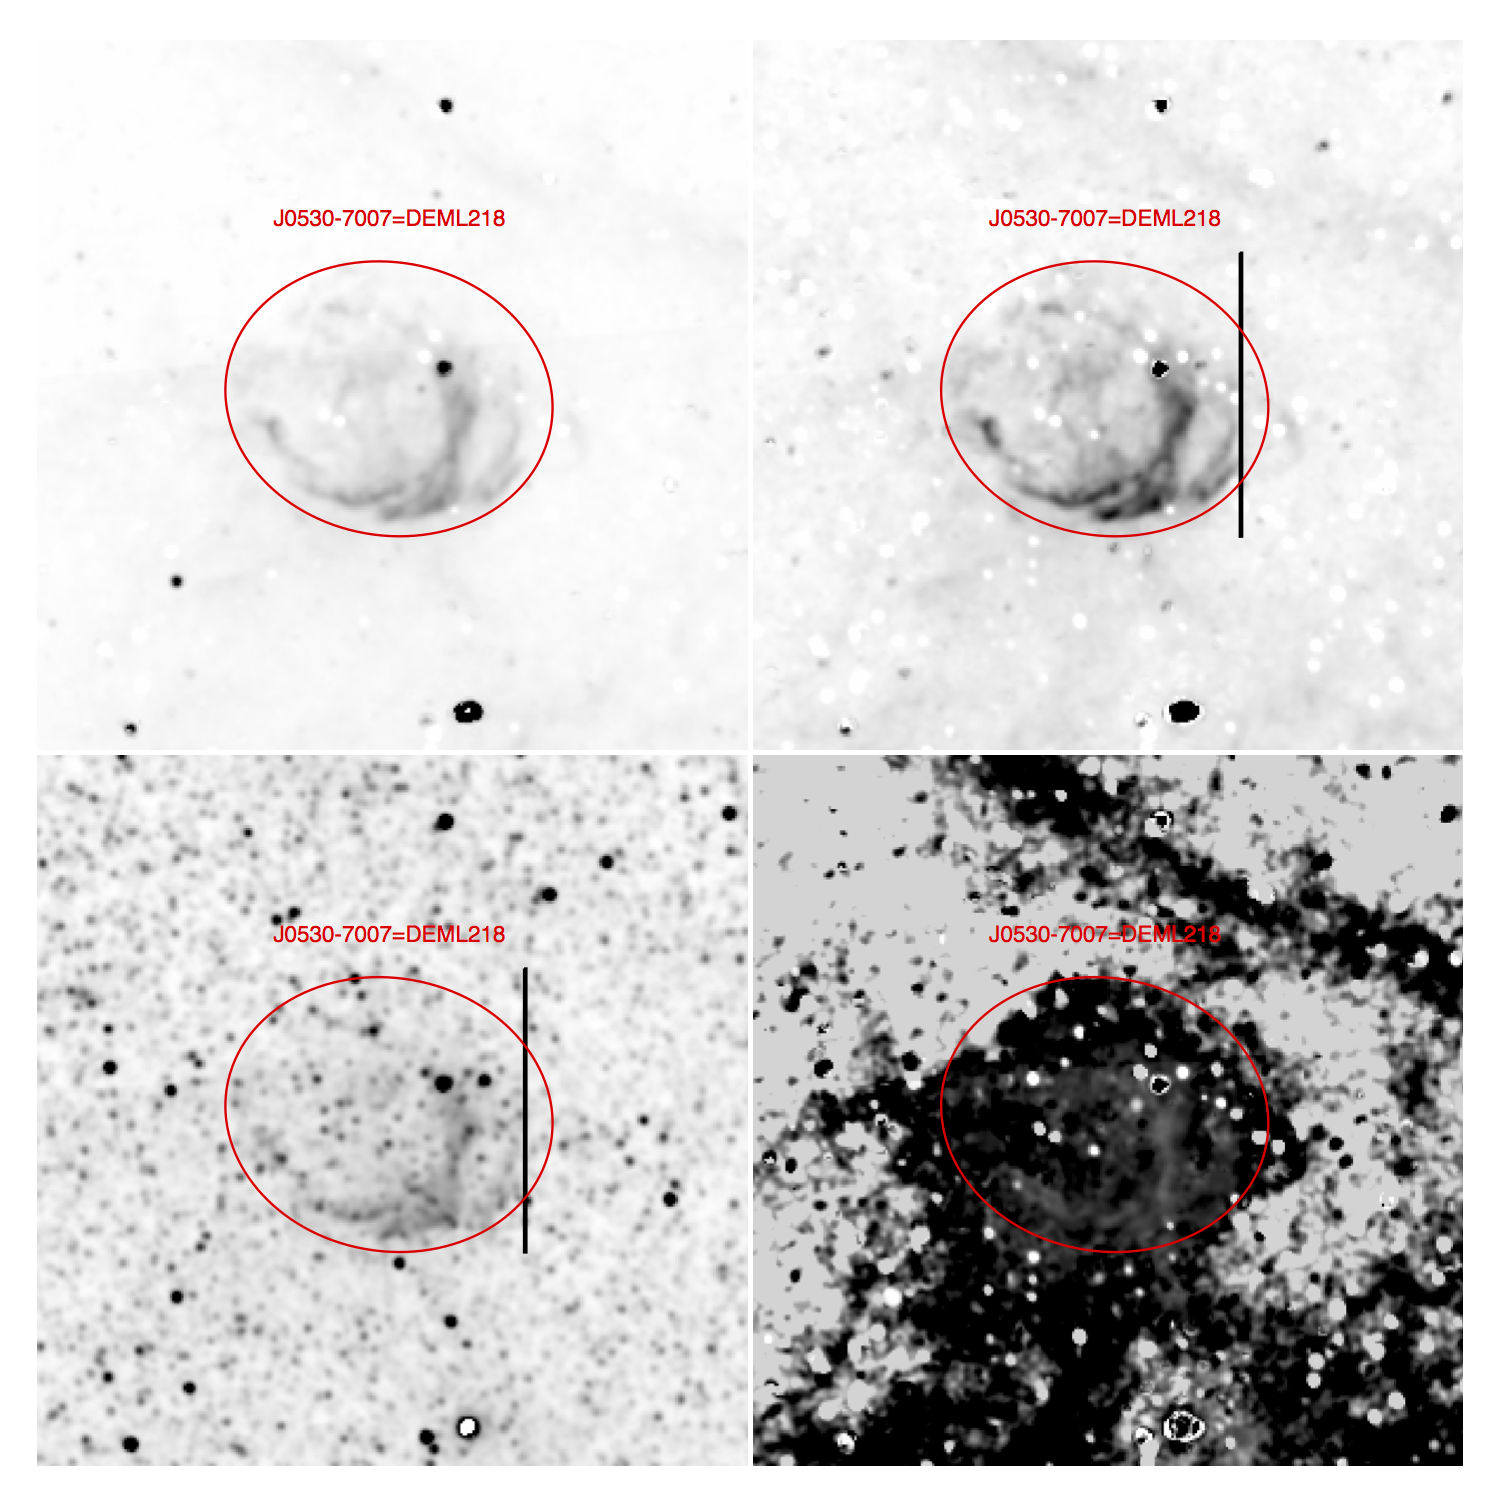
\includegraphics[width=11.cm]{snapshots/J0530-7007.png}
\end{figure}

\newpage
{\bf J0531-7100 = B0532-71.0 = N206}  
 
SNR shell center:   5:31:56.1   -71:00:19.5   

N-S slit; center on bright star NE of shell @ 5:31:23.7  -70:59:20;  offset E 62$^{\prime\prime}$, S 57$^{\prime\prime}$

Scan:  East  175$^{\prime\prime}$

Scan rate:    350$^{\prime\prime}$/hr  for 30 min exposure

Date/Frames:   Nite 3, frames 234-236

Exposure Times:  3 x 30 min

\begin{figure}
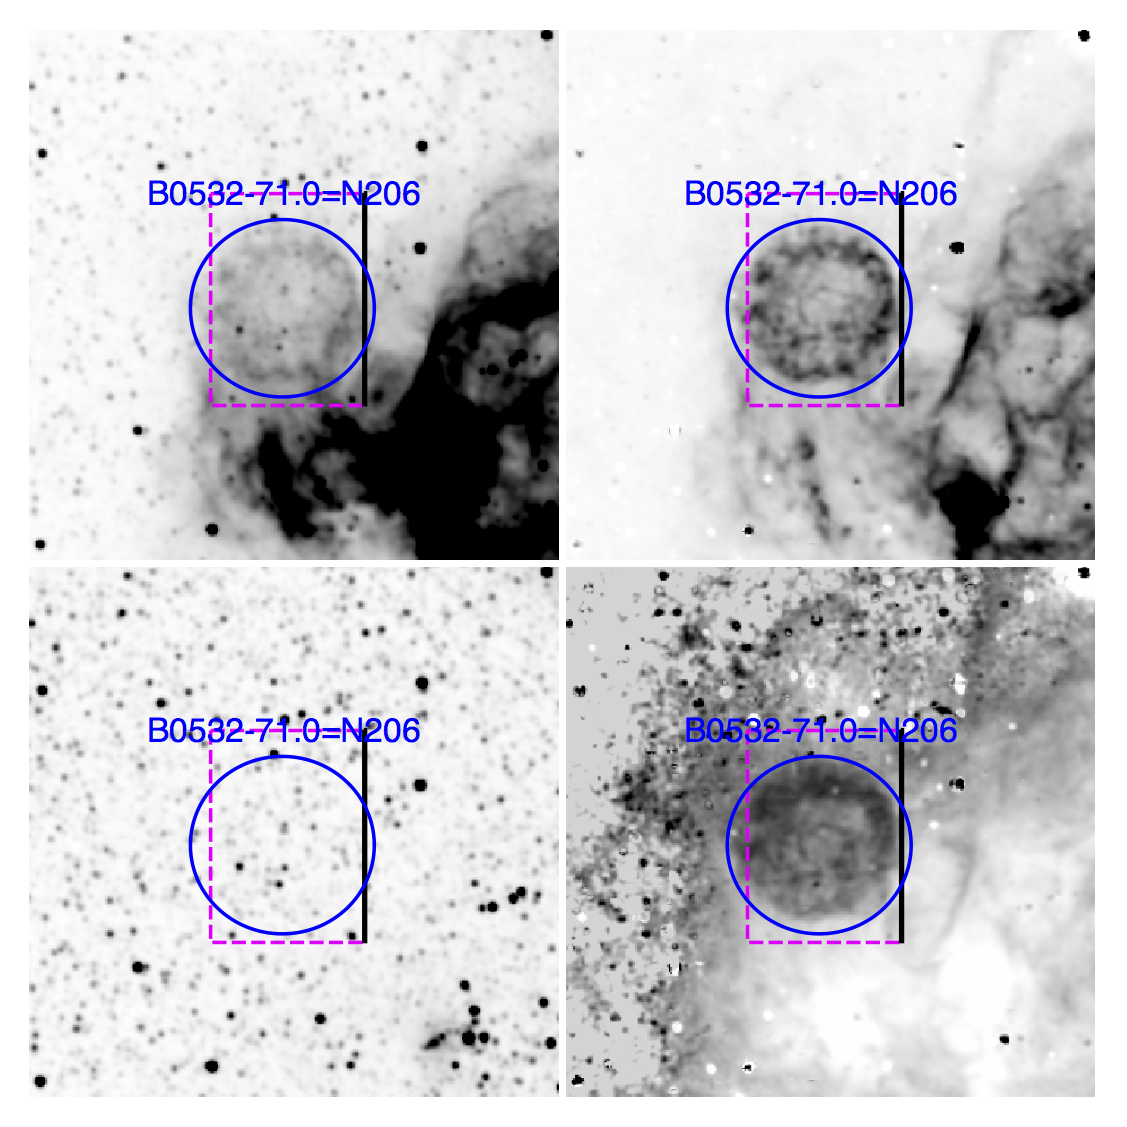
\includegraphics[width=12.5cm]{snapshots/N206.png}
\end{figure}

\newpage
{\bf J0534-6955 = B0534-69.9}  
 
Slit Center:   5:33:51.783  -69:54:44.514  N-S

Scan:  East

Scan rate:  

Date/Frames:

Exposure Times:  

\begin{figure}
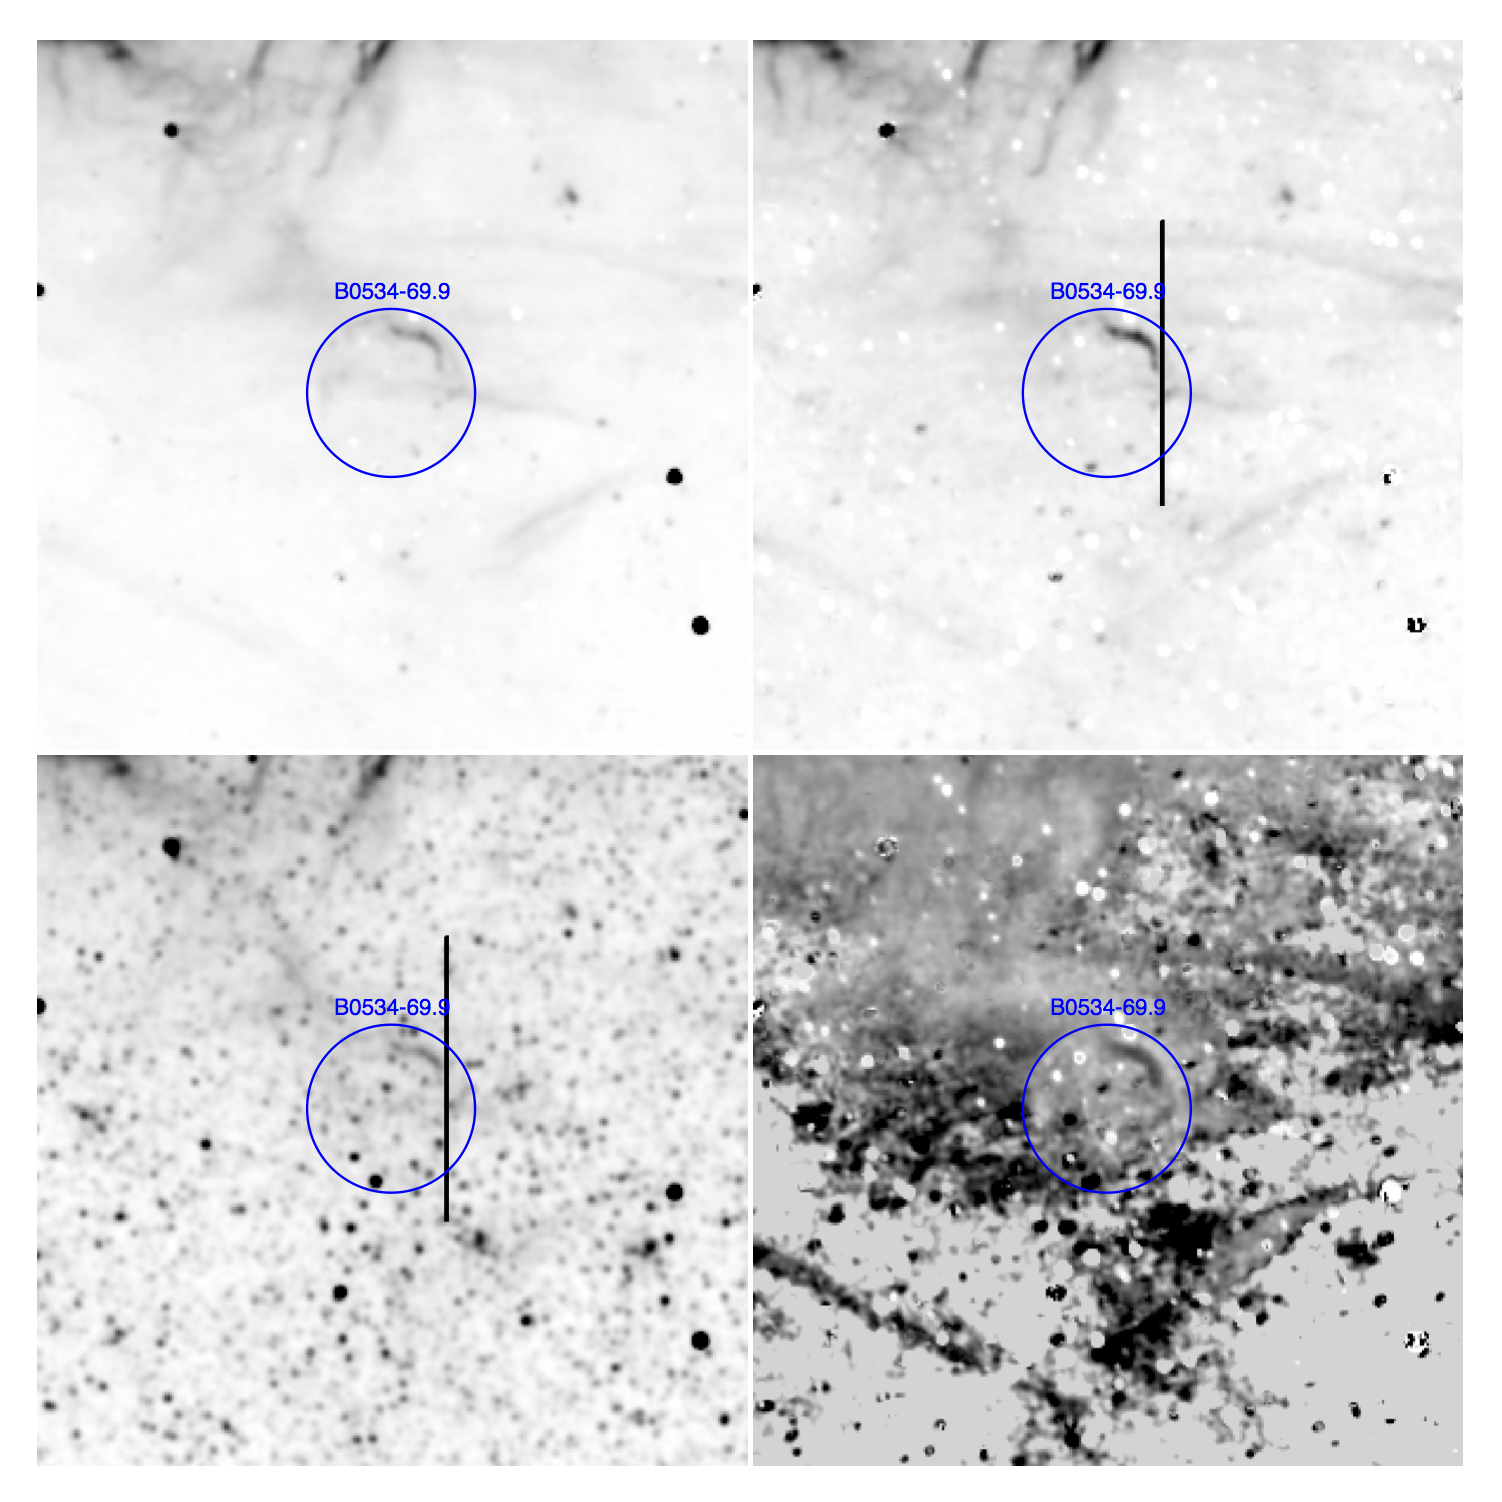
\includegraphics[width=11.cm]{snapshots/B0534-699.png}
\end{figure}

\newpage
{\bf J0534-7033 = B0534-70.5 = DEML238}  
 
Slit Center:   5:34:01.781 -70:33:14.761  N-S

Scan:  East

Scan rate:  

Date/Frames:

Exposure Times:  

\begin{figure}
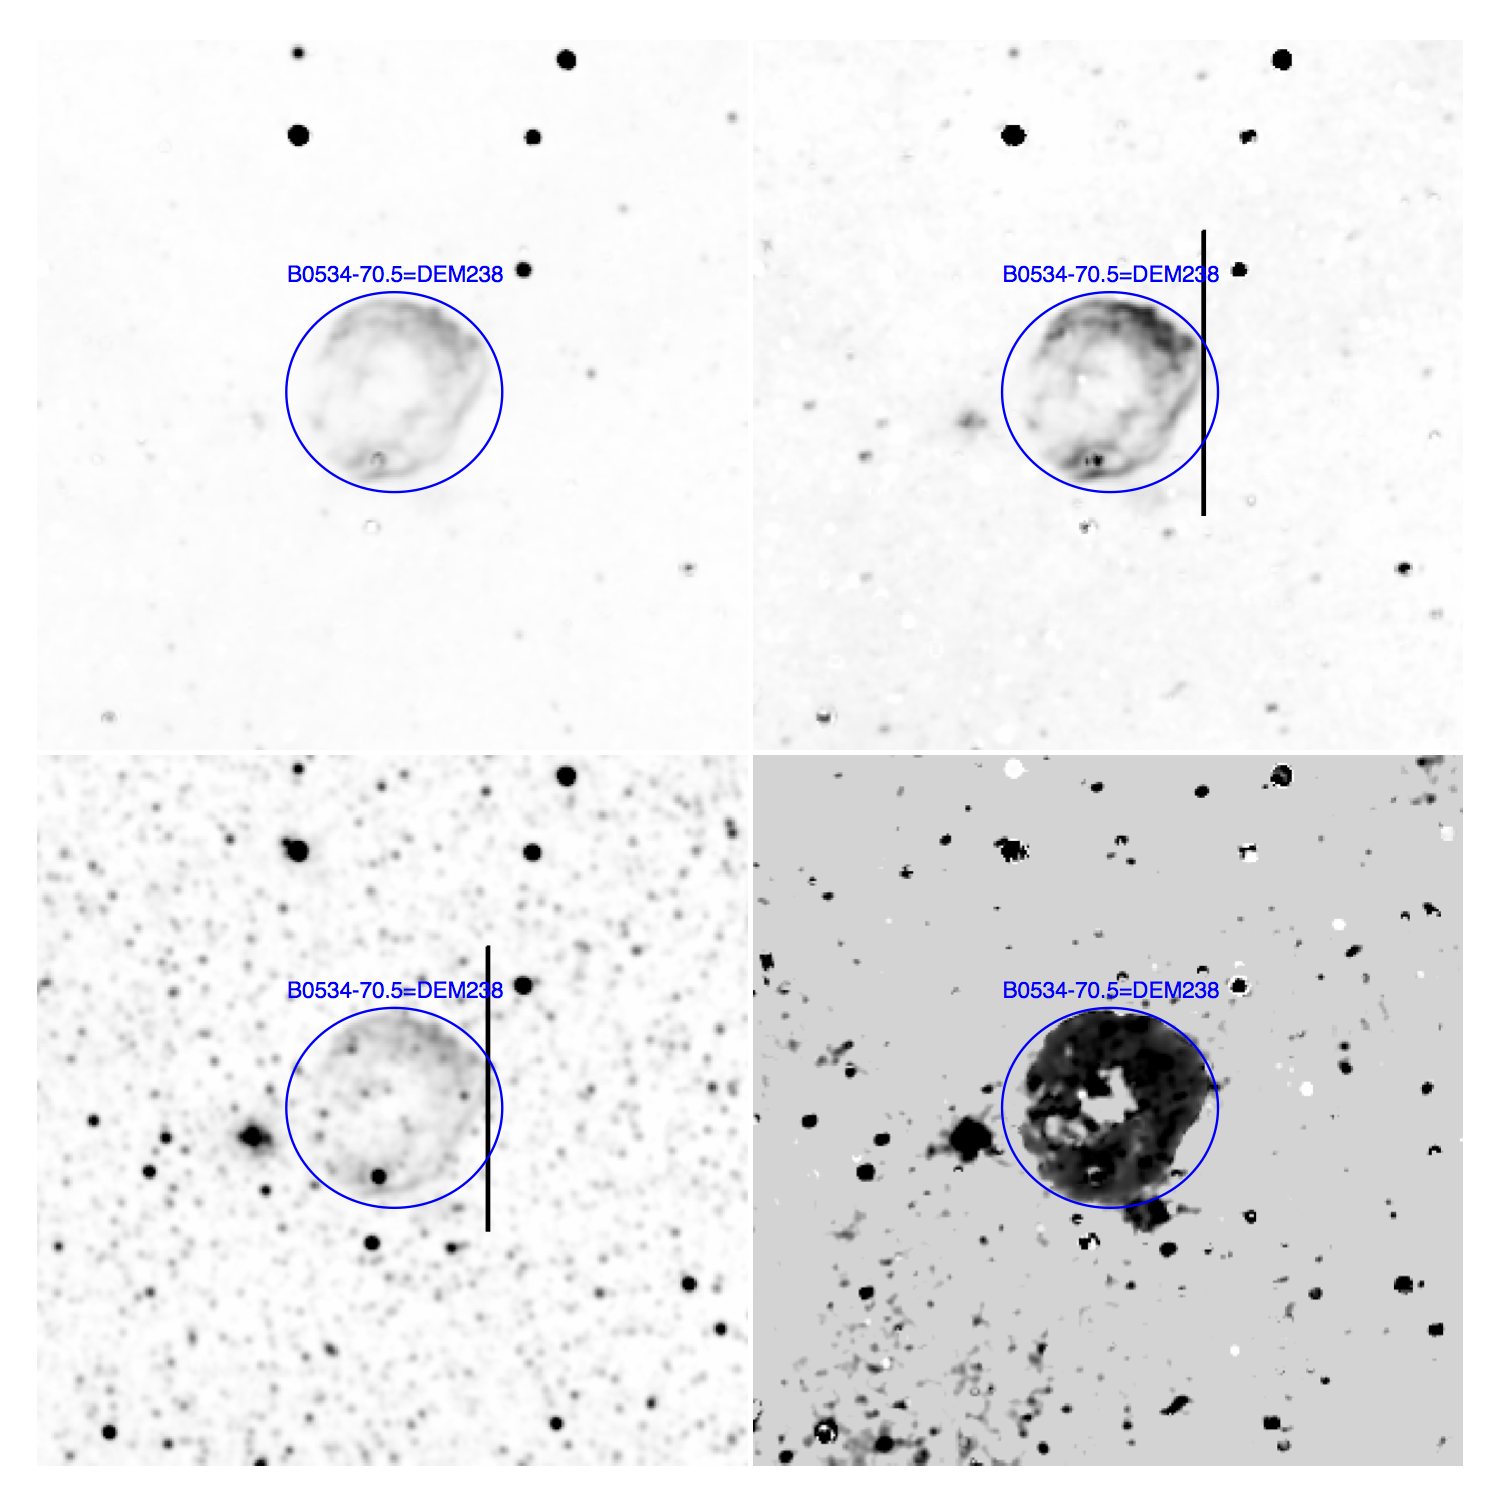
\includegraphics[width=11.cm]{snapshots/B0534-705.png}
\end{figure}

\newpage
{\bf J0535-6602 = N63A = B0535-66.0   (5  arcmin field)}  
 
SNR Center:   5:35:42.2   -66:02:03.7   

E-W slit, center on bright star SW of SNR; offset N 10\arcsec \\
This allows us to isolate the HII region (W lobe) from the SNR (NE and NW lobes)

Scan:  North 45\arcsec

Scan rate:  135\arcsec/hr

Date/Frames:   Nite 1, frames 301-303

Exposure Times:  3 x 20 min

\begin{figure}
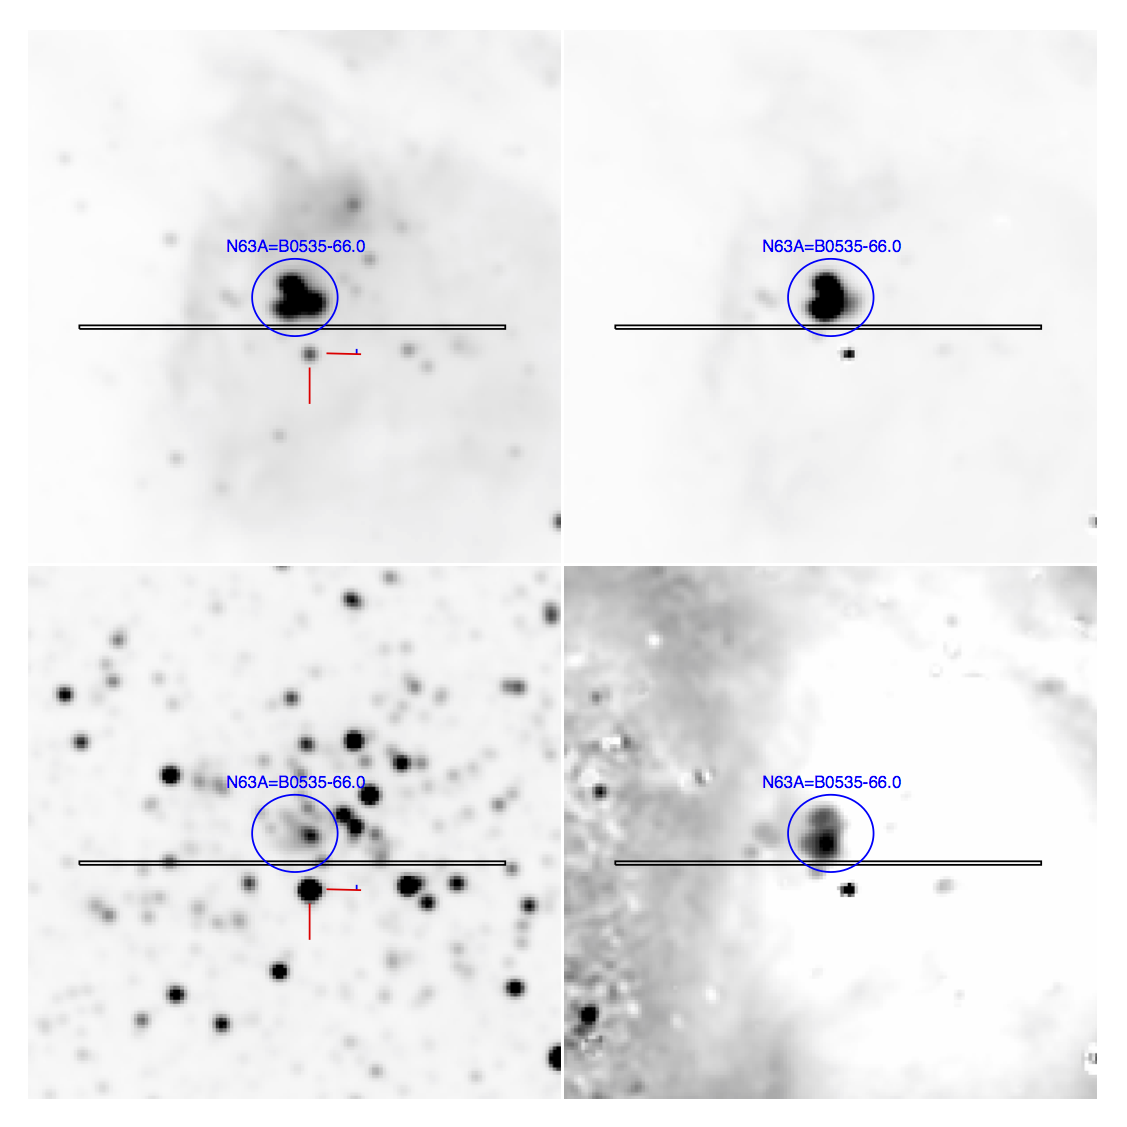
\includegraphics[width=12.5cm]{snapshots/N63A_5arcmin.png}
\end{figure}

\newpage
{\bf J0536-6735 = B0536-67.6}  
 
SNR Center:   5:36:03.639     -67:35:08.228

N-S slit; center just between pair of stars at SE rim; then offset N 38\arcsec

Scan:  West, 125 arcsec

Scan rate: $ -375^{\prime\prime}$/hr for 20 min exposures

Date/Frames:  15 Dec 2018 (UT = nite 2)  3 x 1200 s

Exposure Times:   3 x 20 min

\begin{figure}
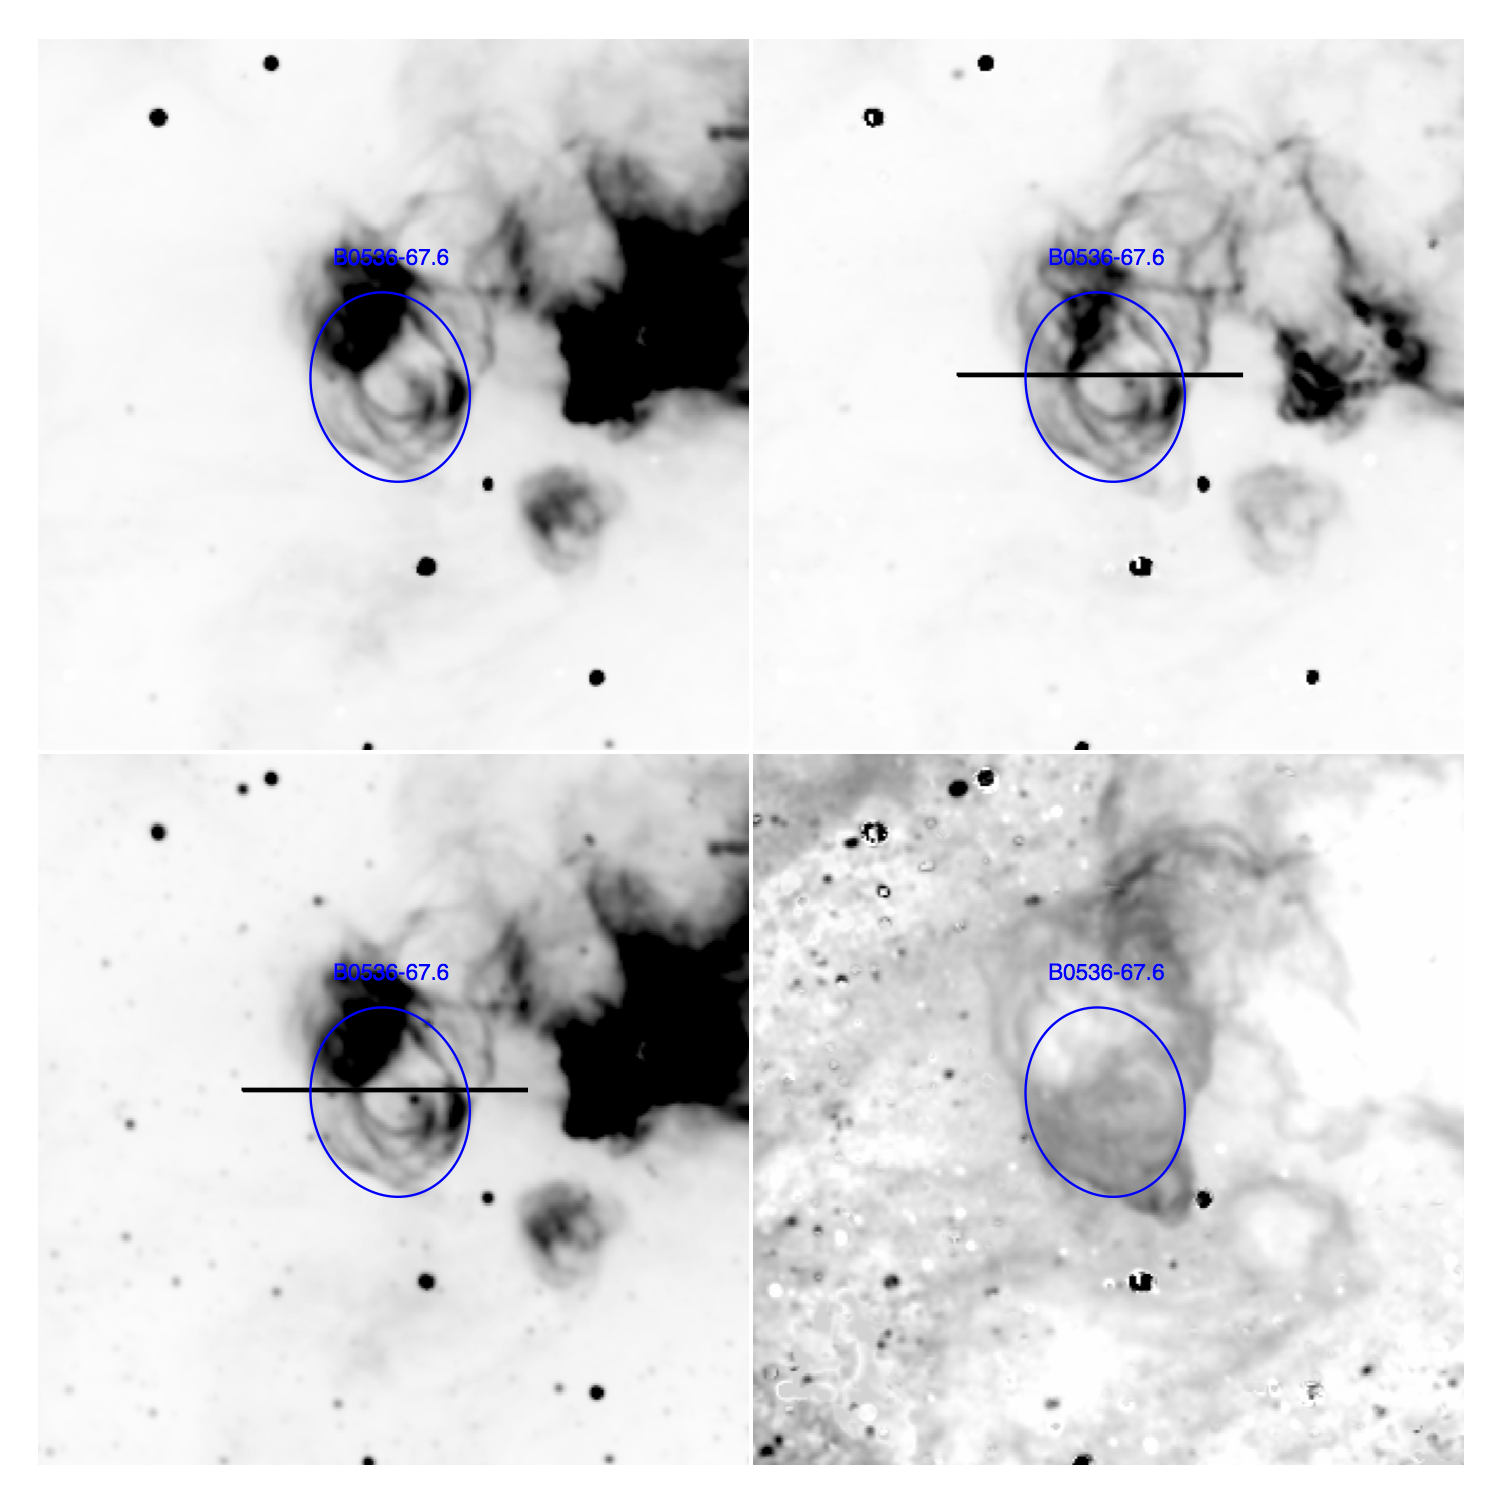
\includegraphics[width=12.5cm]{snapshots/B0536-676.png}
\end{figure}


\newpage
{\bf J0536-7038 = B0536-70.6 = DEM249}  
 
Slit Center:   5:35:50.282   -70:38:35.277 N-S

Scan:  East

Scan rate:  

Date/Frames:

Exposure Times:  

\begin{figure}
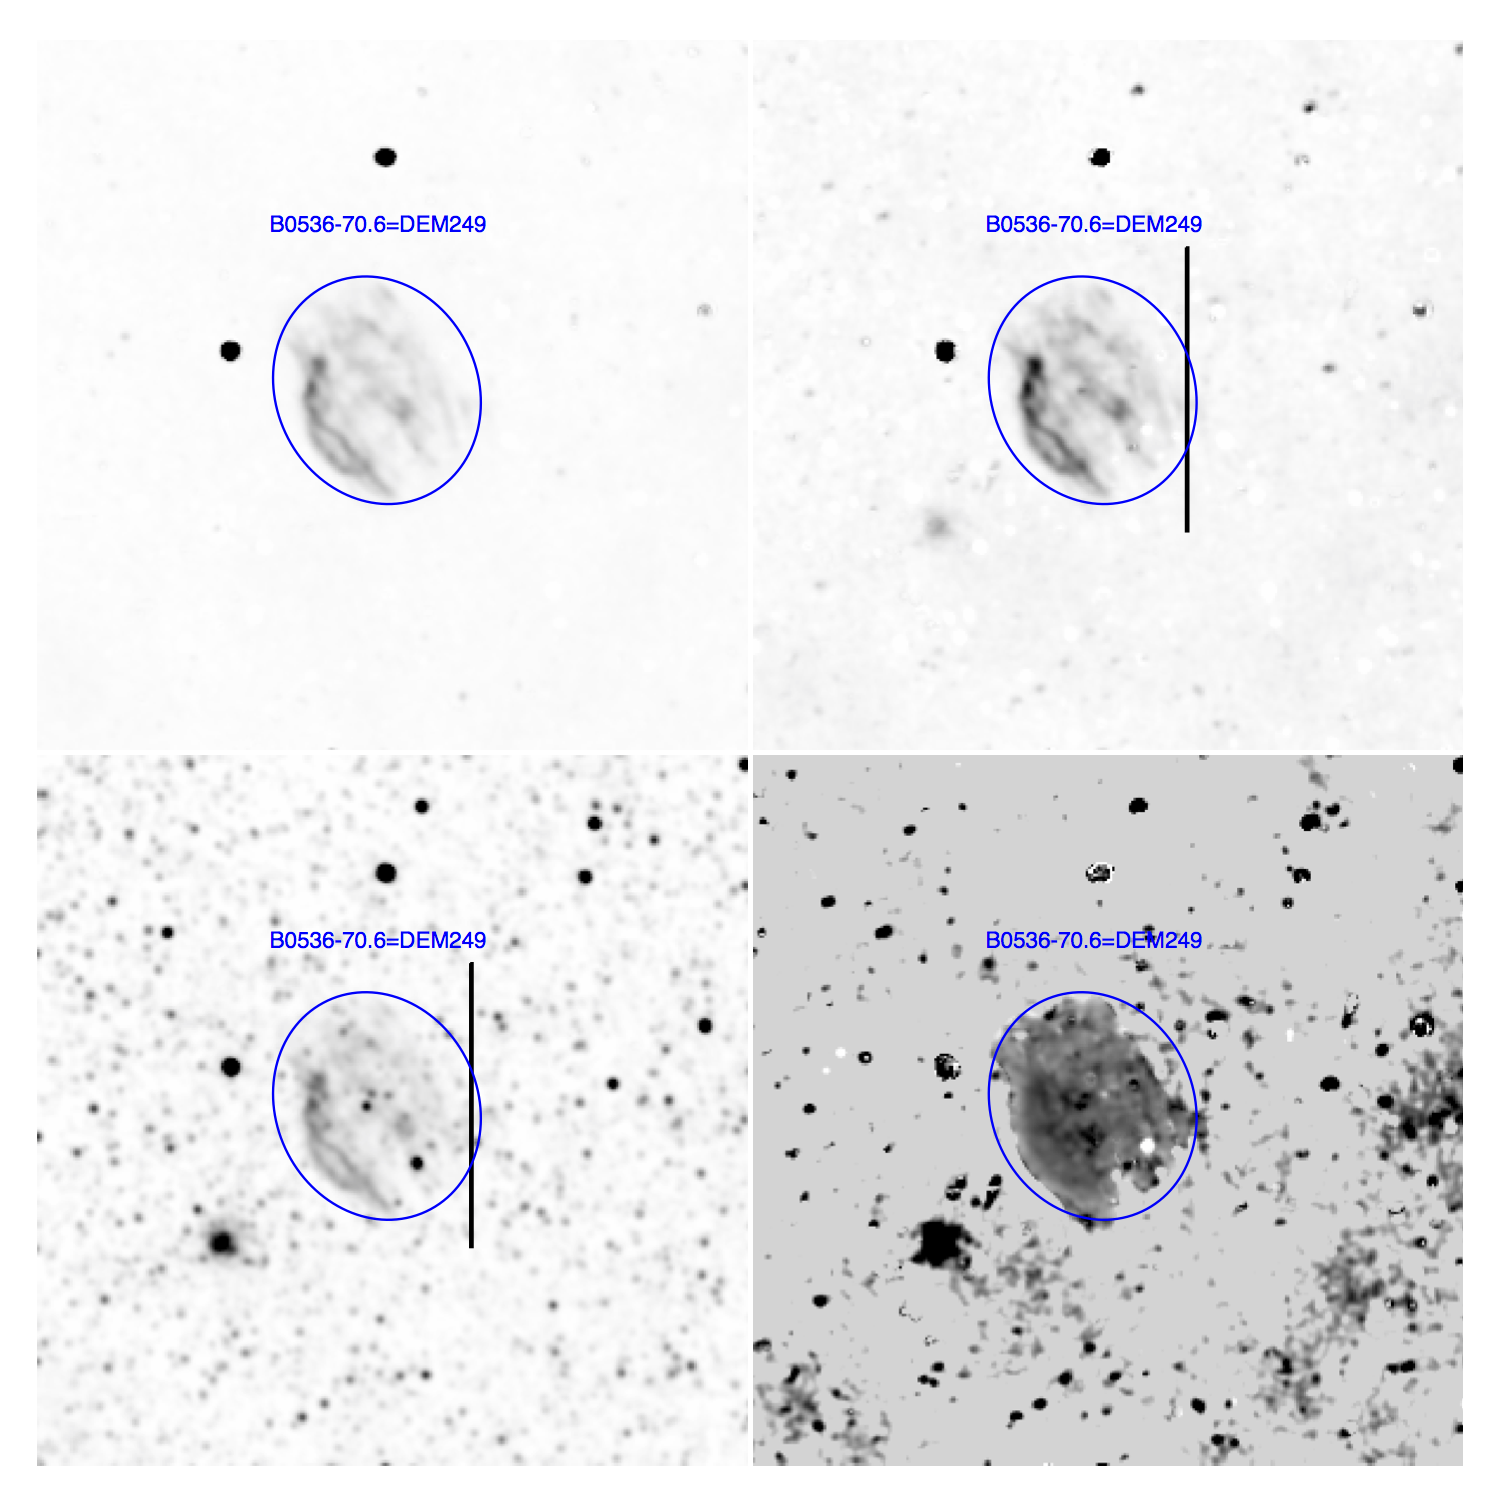
\includegraphics[width=11.cm]{snapshots/B0536-706.png}
\end{figure}


\newpage
{\bf J0537-6639 (new)}  
 
Slit Center:   too big to scan

Scan:  East

Scan rate:  

Date/Frames:

Exposure Times:  

no snapshot
\begin{figure}
%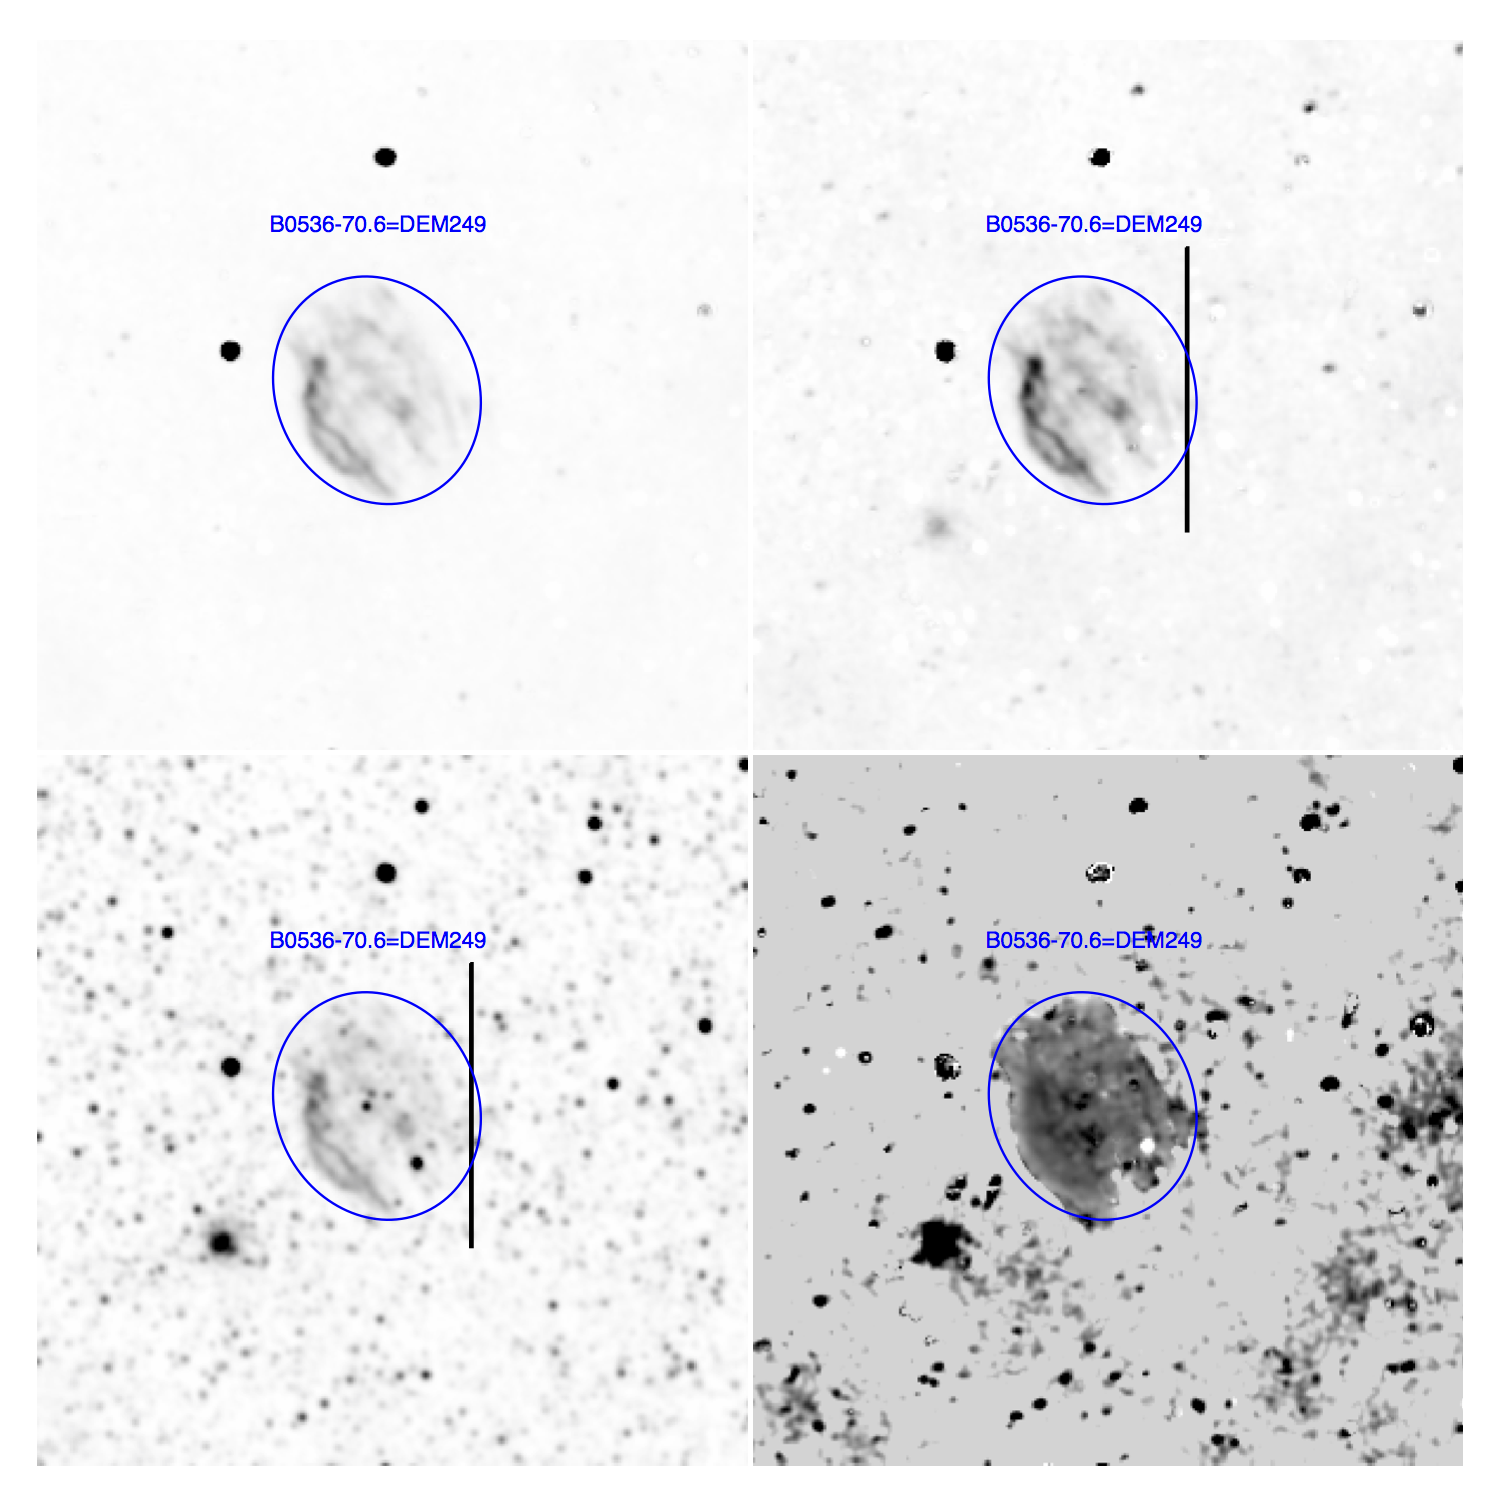
\includegraphics[width=11.cm]{snapshots/B0536-706.png}
\end{figure}

\newpage
{\bf J0537-6627 = DEML256}  
 
SNR Center:  5:37:29.1   -66:27:44.5    

N-S slit; center up on bright star just outside SW rim;  offset W 20$^{\prime\prime}$, N 94$^{\prime\prime}$

Scan:  East, 208$^{\prime\prime}$

Scan rate:  416$^{\prime\prime}$/hr for 30 min exposure

Date/Frames:

Exposure Times:  

\begin{figure}
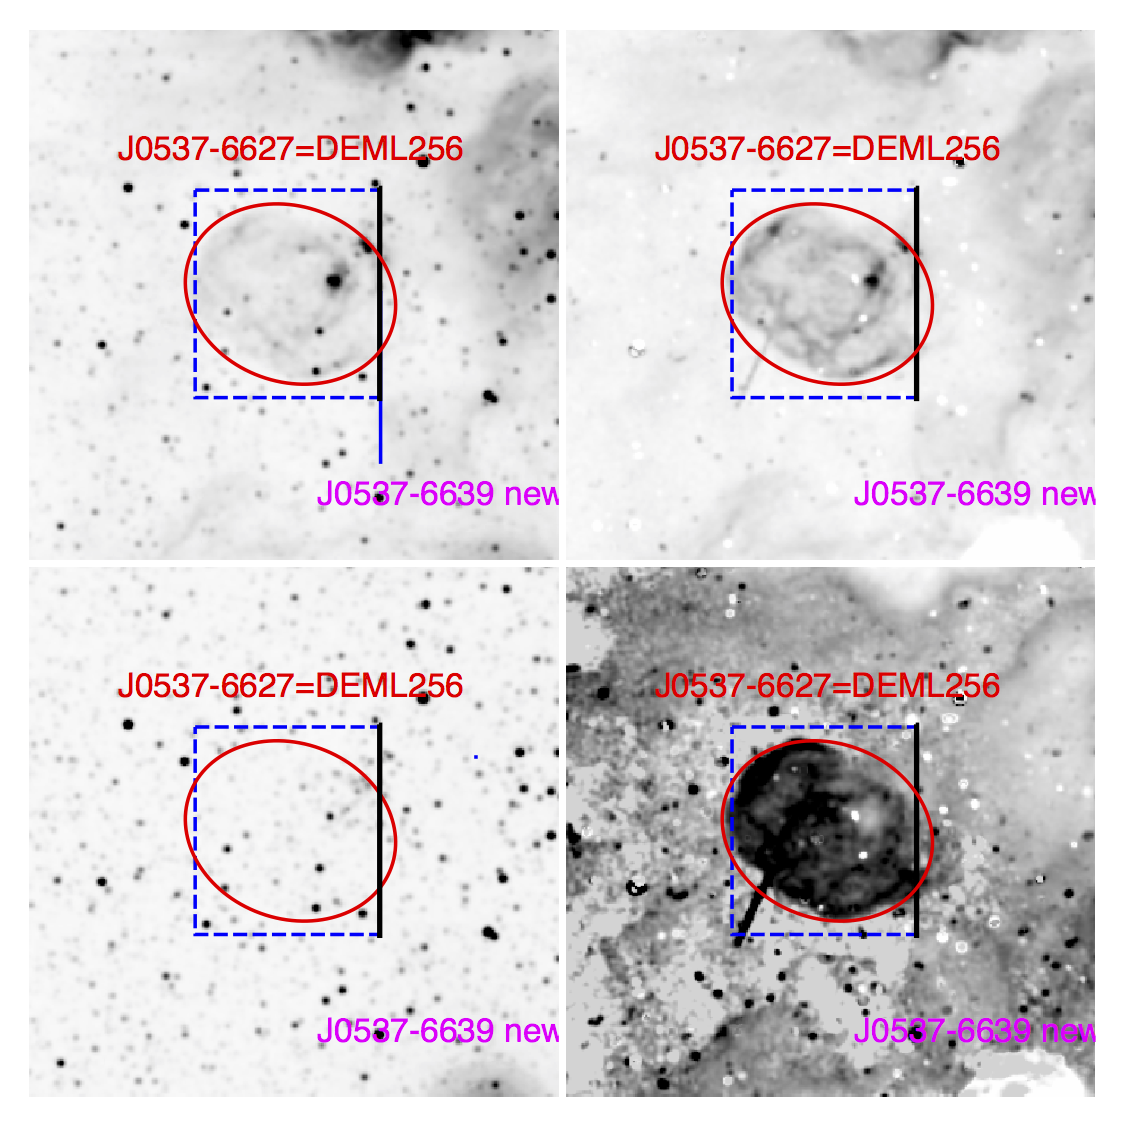
\includegraphics[width=12.5cm]{snapshots/J0537-6627a.png}
\end{figure}

\newpage
{\bf J0538-7004 (new)}  
 
Slit Center:  5:38:39.887  -70:04:13.737 N-S

Scan:  East

Scan rate:  

Date/Frames:

Exposure Times:  

\begin{figure}
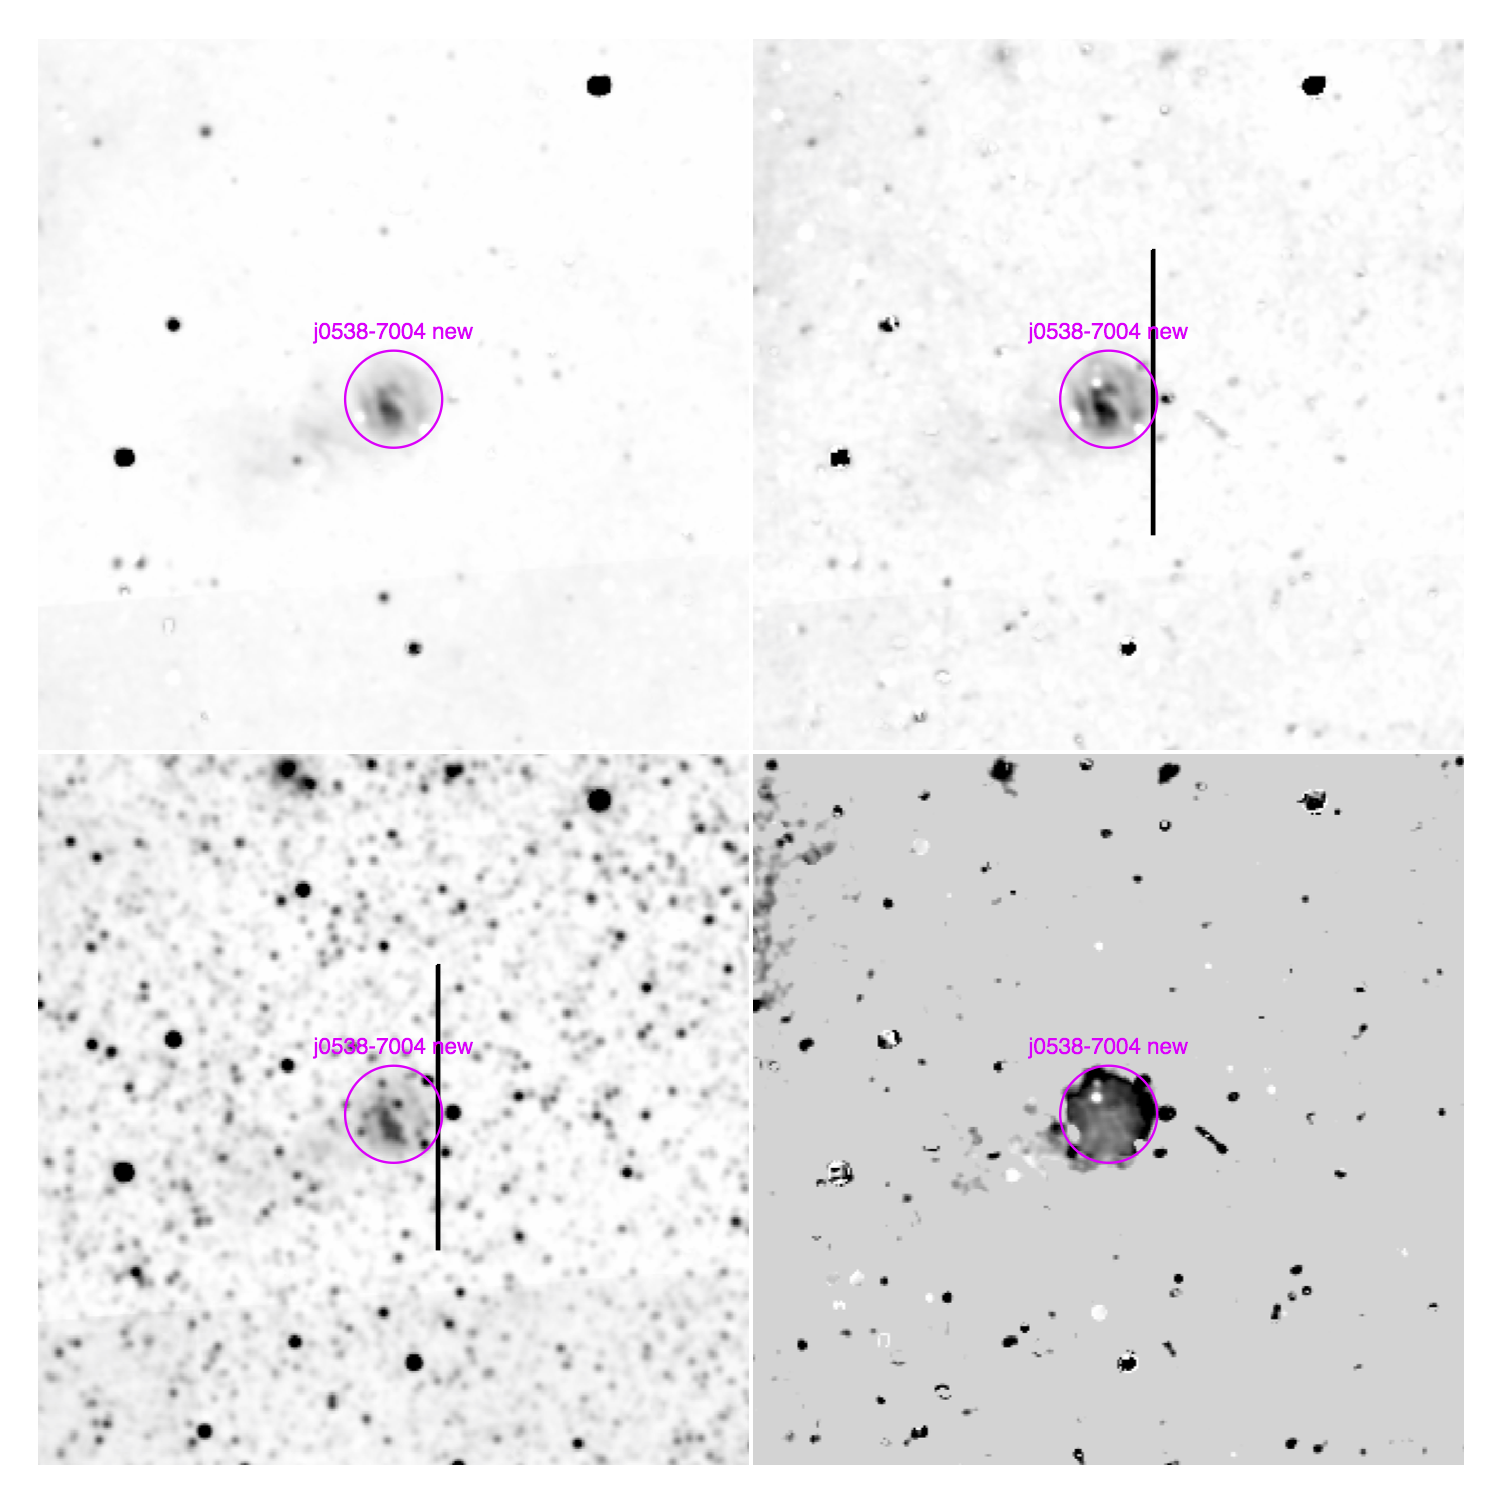
\includegraphics[width=11.cm]{snapshots/J0538-7004.png}
\end{figure}

\newpage
{\bf J0540-6919 = B0540-69.3  (O-rich plerion; 5 arcmin field)}  
 
Slit Center:  5:40:09.612  -69:19:28.770 N-S

Scan:  East

Scan rate:  

Date/Frames:

Exposure Times:  

\begin{figure}
\includegraphics[width=11.cm]{snapshots/B0540-693_5arcmin.png}
\end{figure}

\newpage
{\bf J0543-6858 = B0543-68.9 = DEML299}  
 
Slit Center:  5:43:10.442,-68:57:46.11 E-W

Scan:  South

Scan rate:  

Date/Frames:

Exposure Times:  

\begin{figure}
\includegraphics[width=11.cm]{snapshots/B0543-689.png}
\end{figure}

\newpage 
{\bf This page for DEML316A and 316B (= N135); do these consecutively}

%\vspace{0.1in}
 
%{\bf J0546-6942 = B0547-69.7 = N135 = DEML316B}
{\bf J0547-6941=DEML316A  (smaller one, to east)}

Image Center (for pair):  5:47:09,-69:41:36  N-S slit; offset few \arcsec E and S to marked star

then offset W $\sim 30^{\prime\prime}$, N 36$^{\prime\prime}$   (this was about 16\arcsec W of intended)

Scan:  East 80$^{\prime\prime}$

Scan rate:  160$^{\prime\prime}$/hr for 30 min exposures

Observed Nite 2, frames 247-249:   3 x 30 min
%\vspace{0.1in}

{\bf J0546-6942 = B0547-69.7 = N135 = DEML316B (western one)}

return to start position from above scan; offset S 76$^{\prime\prime}$

Scan:  West 160$^{\prime\prime}$

Scan rate:  $-320 ^{\prime\prime}$/hr for 30 min exposures

Observed Nite 2, frames 253-255:   3 x 30 min
\begin{figure}
\includegraphics[width=10.cm]{snapshots/DEML316ab.png}
\end{figure}

\newpage 

%\vspace{0.1in}
 
%{\bf J0546-6942 = B0547-69.7 = N135 = DEML316B}
{\bf DEML316A/B  longslit}

Setup Star:  5:47:19.2,-69:42:02 (marked star)

P.A. = 20$^\circ$

then offset  S 16.5$^{\prime\prime}$   

  (slit center marked by magenta arrow)

Observe:  2 x 20-30 min
%\vspace{0.1in}

\begin{figure}
\includegraphics[width=12.5cm]{snapshots/DEML316_longslit.png}
\end{figure}

\newpage 
 
 
{\bf J0547-7024 = B0548-70.4 (Balmer-dominated)}

Slit Center:  5:47:38.153   -70:25:05.964  N-S

Scan:  East

Scan rate:  

Date/Frames:

Exposure Times:  

\begin{figure}
\includegraphics[width=11.cm]{snapshots/B0548-704.png}
\end{figure}

\newpage 
 
 
{\bf Hc2, compact H II region (5 arcmin field})   \ \   Surf Brightness 3.7 E-15 ergs/cm$^2/$s/arcsec$^2$

Object Center:  4:54:12.62   -68:21:49   E-W slit

Center on marked star NW of the object; offset E 47\arcsec,  S 44\arcsec

Scan:  South 55\arcsec

Scan rate:  - 165\arcsec/hr\ in Decl. for 1200 s exposures

Date/Frames:

Exposure Times:  

\begin{figure}
\includegraphics[width=12.5cm]{snapshots/Hc2_HII_5arcmin.png}
\end{figure}

\newpage 
 
{\bf Hc10, compact H II region (5 arcmin field})   \ \   Surf Brightness 8.6 E-15 ergs/cm$^2/$s/arcsec$^2$

Object Center:  5:20:33.0    -66:46:43.7   N-S slit

Center on marked star NW of the object; offset E 23\arcsec,  S 63\arcsec

Scan:    East 70\arcsec

Scan rate:  + 210\arcsec/hr\ in R.A. for 1200 s exposures

Date/Frames:

Exposure Times:  

\begin{figure}
\includegraphics[width=12.5cm]{snapshots/Hc10_HII.png}
\end{figure}

\newpage 
 
{\bf Hc20, compact H II region (10 arcmin field})   \ \   Surf Brightness 2.1 E-15 ergs/cm$^2/$s/arcsec$^2$

Object Center:  5:40:42.9    -70:02:30.4   N-S slit

Center on marked star SE of the object; offset W 21\arcsec,  N 84\arcsec

Scan:    West 150\arcsec

Scan rate:  -450\arcsec/hr\ in R.A. for 1200 s exposures

Date/Frames:

Exposure Times:  

\begin{figure}
\includegraphics[width=12.5cm]{snapshots/Hc20_HII.png}
\end{figure}


\end{document}  